\documentclass{book}
\usepackage{graphicx,xcolor}
\usepackage{fancyvrb}
\usepackage[colorlinks=true,urlcolor=blue,linkcolor=cyan]{hyperref}
\usepackage{sidenotes}
\usepackage[toc]{glossaries}
\newglossary[nlg]{variable}{vin}{vot}{List of variables}
\newglossary[nlg]{parameter}{pin}{pot}{List of Parameters}
\makeglossaries
\newcommand{\doclocation}{file:///Users/giulioni/Documents/workspace/gabriele/docs}
\title{GABRIELE}
\author{Gianfranco Giulioni}
\begin{document}
%\maketitle
 
\begin{titlepage}

%	\includegraphics[width=0.15\textwidth]{example-image-1x1}\par\vspace{1cm}
	\begin{center}
	{\color{blue}\scshape\Huge GABRIELE \par}
	\end{center}

	\vspace{2cm}

	\noindent
	{\color{blue}\scshape\Huge G}{\scshape\LARGE eneral} 
	{\color{blue}\scshape\Huge A}{\scshape\LARGE gent} 
	{\color{blue}\scshape\Huge B}{\scshape\LARGE ased}\\
	{\color{blue}\scshape\Huge R}{\scshape\LARGE epast} \hskip7mm 
	{\color{blue}\scshape\Huge I}{\scshape\LARGE mplemented}  
	{\color{blue}\scshape\Huge E}{\scshape\LARGE xtensible}\\
	{\color{blue}\scshape\Huge L}{\scshape\LARGE aboratory} \hskip2.5mm
	{\scshape\large for} \hskip2.5mm
	{\color{blue}\scshape\Huge E}{\scshape\LARGE conomics \par}

%	\begin{tabular}{l l l}
%	{\color{blue}\scshape\Huge G}{\scshape\LARGE eneral}&
%	{\color{blue}\scshape\Huge A}{\scshape\LARGE gent}&
%	{\color{blue}\scshape\Huge B}{\scshape\LARGE ased}\\
%	{\color{blue}\scshape\Huge R}{\scshape\LARGE epast}&
%	{\color{blue}\scshape\Huge I}{\scshape\LARGE mplemented}& 
%	{\color{blue}\scshape\Huge E}{\scshape\LARGE xtensible}\\
%	{\color{blue}\scshape\Huge L}{\scshape\LARGE aboratory}& 
%	{\scshape\large for}&
%	{\color{blue}\scshape\Huge E}{\scshape\LARGE Economics \par}
%	\end{tabular}


 
	
	\vspace{1.5cm}
	\noindent
	{\scshape\Huge Users Manual \par}

	\vspace{2cm}
	\noindent
	{\Large\itshape Gianfranco Giulioni\par}
	\vfill
%	supervised by\par
%	Dr.~Mark \textsc{Brown}

%	\vfill

% Bottom of the page
	{\large \today\par}
\end{titlepage}

\newpage
\thispagestyle{empty}

\null

\newpage
\thispagestyle{empty}

\vspace*{5cm}
\begin{flushright}
	To Gabriele
\end{flushright}

\newpage
\thispagestyle{empty}

\null

\newpage

\pagenumbering{roman}

\tableofcontents
 

\newglossaryentry{var:Yfjf}% label 
{% 
  type=variable,% glossary type 
  name={$Y_{f,j\rightarrow f}$},% 
  description={supply of consumption goods of firm $f$ producing good $j$} 
}
\newglossaryentry{var:Yjc}% label 
{% 
  type=variable,% glossary type 
  name={$Y_{j\rightarrow c}$},% 
  description={supply of consumption goods $j$ in the consumption market} 
}
\newglossaryentry{var:Yfjc}% label 
{% 
  type=variable,% glossary type 
  name={$Y_{f,j\rightarrow c}$},% 
  description={supply of consumption goods of firm $f$ producing good $j$} 
}
\newglossaryentry{var:Dfjf}% label 
{% 
  type=variable,% glossary type 
  name={$D_{f,j\leftarrow f}$},% 
  description={expenditure for investment good received by firm $f$ producing good $j$} 
}
\newglossaryentry{var:ww}% label 
{% 
  type=variable,% glossary type 
  name={$w_{w}$},% 
  description={wage of worker $w$} 
}
\newglossaryentry{var:wwf}% label 
{% 
  type=variable,% glossary type 
  name={$w_{w,f,j}$},% 
  description={wage of worker $w$ hired by firm $f$ producing product $j$} 
}
\newglossaryentry{var:Dc}% label 
{% 
  type=variable,% glossary type 
  name={$D_{c}$},% 
  description={expenditure for consumption possible for consumer $c$ after reallocation of unsatisfied demand} 
}
\newglossaryentry{var:Dfj}% label 
{% 
  type=variable,% glossary type 
  name={$D_{f,j\leftarrow c}$},% 
  description={expenditure for consumption good received by firm $f$ producing good $j$ after reallocation of unsatisfied demand} 
}
\newglossaryentry{var:Dcj}% label 
{% 
  type=variable,% glossary type 
  name={$D_{c,j}$},% 
  description={expenditure for consumption of good $j$ possible for consumer $c$ after reallocation of unsatisfied demand} 
}
\newglossaryentry{var:Dj}% label 
{% 
  type=variable,% glossary type 
  name={$D_{j\leftarrow c}$},% 
  description={Demand of good $j$ after reallocation of unsatisfied demand} 
}
\newglossaryentry{var:Yj}% label 
{% 
  type=variable,% glossary type 
  name={$Y_{j}$},% 
  description={production of good $j$: sum of the production of all firms producing product $j$} 
}
\newglossaryentry{var:Yfj}% label 
{% 
  type=variable,% glossary type 
  name={$Y_{f,j}$},% 
  description={production of firm $f$ producing good $j$} 
}
\newglossaryentry{var:Dafjc}% label 
{% 
  type=variable,% glossary type 
  name={$D^a_{f,j\leftarrow c}$},% 
  description={sum of expenditure for consumption received by firm $f$ producing good $j$} 
}
\newglossaryentry{var:Dajc}% label 
{% 
  type=variable,% glossary type 
  name={$D^a_{j\leftarrow c}$},% 
  description={sum of expenditure for consumption of good $j$ possible for all consumers} 
}
\newglossaryentry{var:Dacj}% label 
{% 
  type=variable,% glossary type 
  name={$D^a_{c,j}$},% 
  description={expenditure for consumption of good $j$ possible for consumer $c$ considering his/her financial resources. It is lower than desired consumption for credit constrained consumers} 
}
\newglossaryentry{var:Dac}% label 
{% 
  type=variable,% glossary type 
  name={$D^a_{c}$},% 
  description={expenditure for consumption possible for consumer $c$ considering his/her financial resources. It is lower than desired consumption for credit constrained consumers} 
}
\newglossaryentry{var:BAac}% label 
{% 
  type=variable,% glossary type 
  name={$BA^a_{c}$},% 
  description={the amount allowed by consumer's $c$ best bank after s/he asked for credit} 
}
\newglossaryentry{var:BAdc}% label 
{% 
  type=variable,% glossary type 
  name={$BA^d_{c}$},% 
  description={the account desired by consumer $c$ in his best bank when s/he asks for additional credit} 
}
\newglossaryentry{var:alphacj}% label 
{% 
  type=variable,% glossary type 
  name={$\alpha_{c,j}$},% 
  description={share of expenditure on consumption goods $j$ desired by consumer $c$. It is an index of the consumers appreciation for the given item} 
}
\newglossaryentry{var:Ddcj}% label 
{% 
  type=variable,% glossary type 
  name={$D^{d}_{c,j}$},% 
  description={expenditure on consumption goods $j$ desired by consumer $c$} 
}
\newglossaryentry{var:Ddc}% label 
{% 
  type=variable,% glossary type 
  name={$D^{d}_{c}$},% 
  description={total expenditure on consumption goods desired by consumer $c$} 
}
\newglossaryentry{var:BAdb}% label 
{% 
  type=variable,% glossary type 
  name={$BA^{db}$},% 
  description={amount of a bank account desired by bank} 
}
\newglossaryentry{var:isub-}% label 
{% 
  type=variable,% glossary type 
  name={$i_{sub}^-$},% 
  description={subsidized interest rate on negative bank account with negative amount (loans)} 
}
\newglossaryentry{var:i-}% label 
{% 
  type=variable,% glossary type 
  name={$i^-$},% 
  description={interest rate on negative bank account with negative amount (loans)} 
}
\newglossaryentry{var:i+}% label 
{% 
  type=variable,% glossary type 
  name={$i^+$},% 
  description={interest rate on bank account with positive amount (deposits)} 
}
\newglossaryentry{var:Db}% label 
{% 
  type=variable,% glossary type 
  name={$D_b$},% 
  description={deposits of bank $b$. It corresponds to one of the liabilities in the bank balance sheet: $L_b=E_b+D_b$} 
}
\newglossaryentry{var:Eb}% label 
{% 
  type=variable,% glossary type 
  name={$E_b$},% 
  description={equity base of bank $b$. It corresponds to one of the liabilities in the bank balance sheet: $L_b=E_b+D_b$} 
}
\newglossaryentry{var:Lb}% label 
{% 
  type=variable,% glossary type 
  name={$L_b$},% 
  description={loans extended by bank $b$. It corresponds to assets of the bank balance sheet: $L_b=E_b+D_b$} 
}
\newglossaryentry{var:BA-}% label 
{% 
  type=variable,% glossary type 
  name={$BA^-$},% 
  description={a negative bank account: loan} 
}
\newglossaryentry{var:BA+}% label 
{% 
  type=variable,% glossary type 
  name={$BA^+$},% 
  description={a positive bank account: deposit} 
}
\newglossaryentry{var:BAcb}% label 
{% 
  type=variable,% glossary type 
  name={$BA_{cb}$},% 
  description={bank account of consumer $c$ in bank $b$} 
}
\newglossaryentry{var:BAfb}% label 
{% 
  type=variable,% glossary type 
  name={$BA_{fb}$},% 
  description={bank account of firm $f$ in bank $b$} 
}
\newglossaryentry{var:Bf}% label 
{% 
  type=variable,% glossary type 
  name={$B_{f}$},% 
  description={debt of firm $f$. Its a liability in the firm balance sheet: $K_f=E_f+B_f$} 
}
\newglossaryentry{var:Ef}% label 
{% 
  type=variable,% glossary type 
  name={$E_{f}$},% 
  description={equity base of firm $f$. It is a liability in the firm balance sheet: $K_f=E_f+B_f$} 
}
\newglossaryentry{var:YPc}% label 
{% 
  type=variable,% glossary type 
  name={$Y^{P}_{c}$},% 
  description={potential production of consumer $c$ as a worker} 
}
\newglossaryentry{var:nsye}% label 
{% 
  type=variable,% glossary type 
  name={$n_{c,sye}$},% 
  description={number of successful period of education achieved by consumer $c$ during its school period} 
}
\newglossaryentry{var:YPLf}% label 
{% 
  type=variable,% glossary type 
  name={$Y^{PL}_{f}$},% 
  description={potential production that could be realized by firm $f$ with the current level of workforces an no production capital constraint} 
}
\newglossaryentry{var:YPKf}% label 
{% 
  type=variable,% glossary type 
  name={$Y^{PK}_{f}$},% 
  description={potential production that could be realized by firm $f$ with the current level of production capital and no labor constrain} 
}
\newglossaryentry{var:Kf}% label 
{% 
  type=variable,% glossary type 
  name={$K_{f}$},% 
  description={production capital of firm $f$. It gives the assets in the firm balance sheet: $K_f=E_f+B_f$} 
}
\newglossaryentry{var:Yf}% label 
{% 
  type=variable,% glossary type 
  name={$Y_{f}$},% 
  description={production realized by firm $f$} 
}
\newglossaryentry{var:psif}% label 
{% 
  type=variable,% glossary type 
  name={$\psi_{f}$},% 
  description={sum of productivities of all workers hired by firm $f$} 
}
\newglossaryentry{var:psiwf}% label 
{% 
  type=variable,% glossary type 
  name={$\psi_{w,f}$},% 
  description={productivity of worker $w$ hired by firm $f$} 
}
\newglossaryentry{var:psic}% label 
{% 
  type=variable,% glossary type 
  name={$\psi_{c}$},% 
  description={productivity of consumer $c$ reached during school time} 
}
\newglossaryentry{var:Wfj}% label 
{% 
  type=variable,% glossary type 
  name={$W_{f,j}$},% 
  description={Sum of wages payed by firm $f$ producing good $j$} 
}
\newglossaryentry{var:pifj}% label 
{% 
  type=variable,% glossary type 
  name={$\pi_{f,j}$},% 
  description={economic result of firm $f$ producing good $j$. A poistive conomic result is called profit while a negative one is called loss} 
}
 \newglossaryentry{var:Dff}% label 
{% 
  type=variable,% glossary type 
  name={$D_{f,j\leftarrow f}$},% 
  description={Demand of goods for investment purpose} 
}

\newglossaryentry{par:thetanbcc}{% 
  type=parameter,% glossary type 
  name={$\theta_{nbcc}$},% 
  description={number of bank accounts hold by consumers} 
}
\newglossaryentry{par:thetamincba}{% 
  type=parameter,% glossary type 
  name={$\theta_{mincba}$},% 
  description={minimum amount in each consumers' bank account at initialization} 
}
\newglossaryentry{par:thetamaxcba}{% 
  type=parameter,% glossary type 
  name={$\theta_{maxcba}$},% 
  description={minimum amount in each consumers' bank account at initialization} 
}


\newglossaryentry{par:thetaptbub}% label 
{% 
  type=parameter,% glossary type 
  name={$\theta_{ptbub}$},% 
  description={probability that a non student consumer working state is initialized as unemployed} 
}
\newglossaryentry{par:thetamnpe}% label 
{% 
  type=parameter,% glossary type 
  name={$\theta_{mnpe}$},% 
  description={maximum periods of school education possible in the system} 
}
\newglossaryentry{par:thetamnfpe}% label 
{% 
  type=parameter,% glossary type 
  name={$\theta_{mnfpe}$},% 
  description={number of failed periods of education after which a student leaves school} 
}
\newglossaryentry{par:thetacea}% label 
{% 
  type=parameter,% glossary type 
  name={$\theta_{cea}$},% 
  description={consumer exit age} 
}
\newglossaryentry{par:thetaminas}% label 
{% 
  type=parameter,% glossary type 
  name={$\theta_{minas}$},% 
  description={minimum of the ability of a consumer as a student} 
}
\newglossaryentry{par:thetamaxas}% label 
{% 
  type=parameter,% glossary type 
  name={$\theta_{maxas}$},% 
  description={maximum of the ability of a consumer as a student} 
}
\newglossaryentry{par:Thetaas}% label 
{% 
  type=parameter,% glossary type 
  name={$\Theta_{as}$},% 
  description={distribution of the abilities of consumers as students} 
}
\newglossaryentry{par:thetaas}% label 
{% 
  type=parameter,% glossary type 
  name={$\theta_{c,as}$},% 
  description={ability of a consumer as a student} 
}
 
\newglossaryentry{par:thetaYL}% label 
{% 
  type=parameter,% glossary type 
  name={$\theta_{YL}$},% 
  description={parameter of total workers productivity in production function} 
}
 


%A \gls{not:set} is a collection of objects.

\printglossaries

\clearpage
\thispagestyle{empty}
\pagenumbering{arabic}
%\section{Coding}
%You can try your main loop without scheduling events by setting the \verb+schedulingFlag+ to false.

\part{Setting up GABRIELE}


In this part of the manual we describe two ways of setting up for running simulations. The first one is the standard Repast procedure, where one can take advantage of various wizards to set up and run simulations. Although this provides several facilities, some user could feel uncomfortable with this standard process and would like to revert to a more basic procedure. The streamlined installation is for these users. It behooves to point out that the streamlined procedure was especially designed for running the model in the local machine and in batch mode. Therefore, the supporters of the Unix like command line interface will appreciate it. To help clarifying, it is worth to say that the streamlined procedure was developed to avoid the slowness of the wizards when continuously checking the effects of introducing new lines of code. It allows to run the model from the command line by typing two keys (i.e arrow up key - to recall the execution command, and the enter key). 
%An efficient way to process is thus to use the streamlined procedure during the development phase and for local simulation. 


\chapter{Standard Installation}
\section{Installation}

In this section we describe the standard installation process needed to prepare the system to run simulations. After taking the steps described below, the user should be able to run the model regardless of the operative system s/he is using.

The model needs Repast Symphony (RS), who in turn needs the Java Development Kit (JDK). Therefore we need first to check if the JDK is installed in the system and install it if needed. Once JDK is properly running, we have to install RS. Finally the model can be installed and run in RS.

\subsection{Java Development Kit (JDK)}

Check the list of installed software to know if JDK is installed in your system. If yes, note the JDK version.
Alternatively, you can open the command line interface of your system, type \verb+javac -version+ and hit the return key. 

Once verified if JDK is installed and, if yes, its version, visit the following URL:\\
\url{http://www.oracle.com/technetwork/java/javase/downloads/index.html}\\
to know which is latest released version of JDK.

If JDK is not installed in your system or if it is not at the latest release, follow the instruction found in the JDK download page to install or upgrade it. You can also search the internet for alternative ways to install or upgrade the JDK on your system.

This installation phase is complete when the \verb+javac -version+ command returns what you expect.
If not, you should fist check if the folder containing the JDK executables are in your execution path and add it manually if needed.
Furthermore, some Linux distribution must be informed on which JDK to use using the \verb+update-alternatives+ command. 

\subsection{Repast Simphony (RS)}

The Repast suite website: \url{http://repast.sourceforge.net} has all the information needed to download and install RS.

Note that RS is provided as a plugin of the eclipse Integrated Development Environment. The Repast development team provides a customized version of eclipse, so you could encounter problems with already installed versions of eclipse. Note that the streamlined installation provided below show how to avoid using eclipse.

\subsection{GABRIELE}

GABRIELE has to be installed as an eclipse RS project. We will give hereafter the instructions to achieve this goal.

First of all, open eclipse.% downloaded and installed as described in the previous section.

Suppose your workspace has the following path:\\
\verb+/Users/coolcoder/Documents/workspace+

Open the RS perspective (window $\rightarrow$ open perspective).

Create a new RS project called \verb+gabriele+ (file $\rightarrow$ new $\rightarrow$ Repast Simphony project)

This creates the \verb+gabriele+ folder and a series of sub folders inside the workspace:

The following figure show the \verb+gabriele+ project folders tree.

\vskip2mm
\noindent
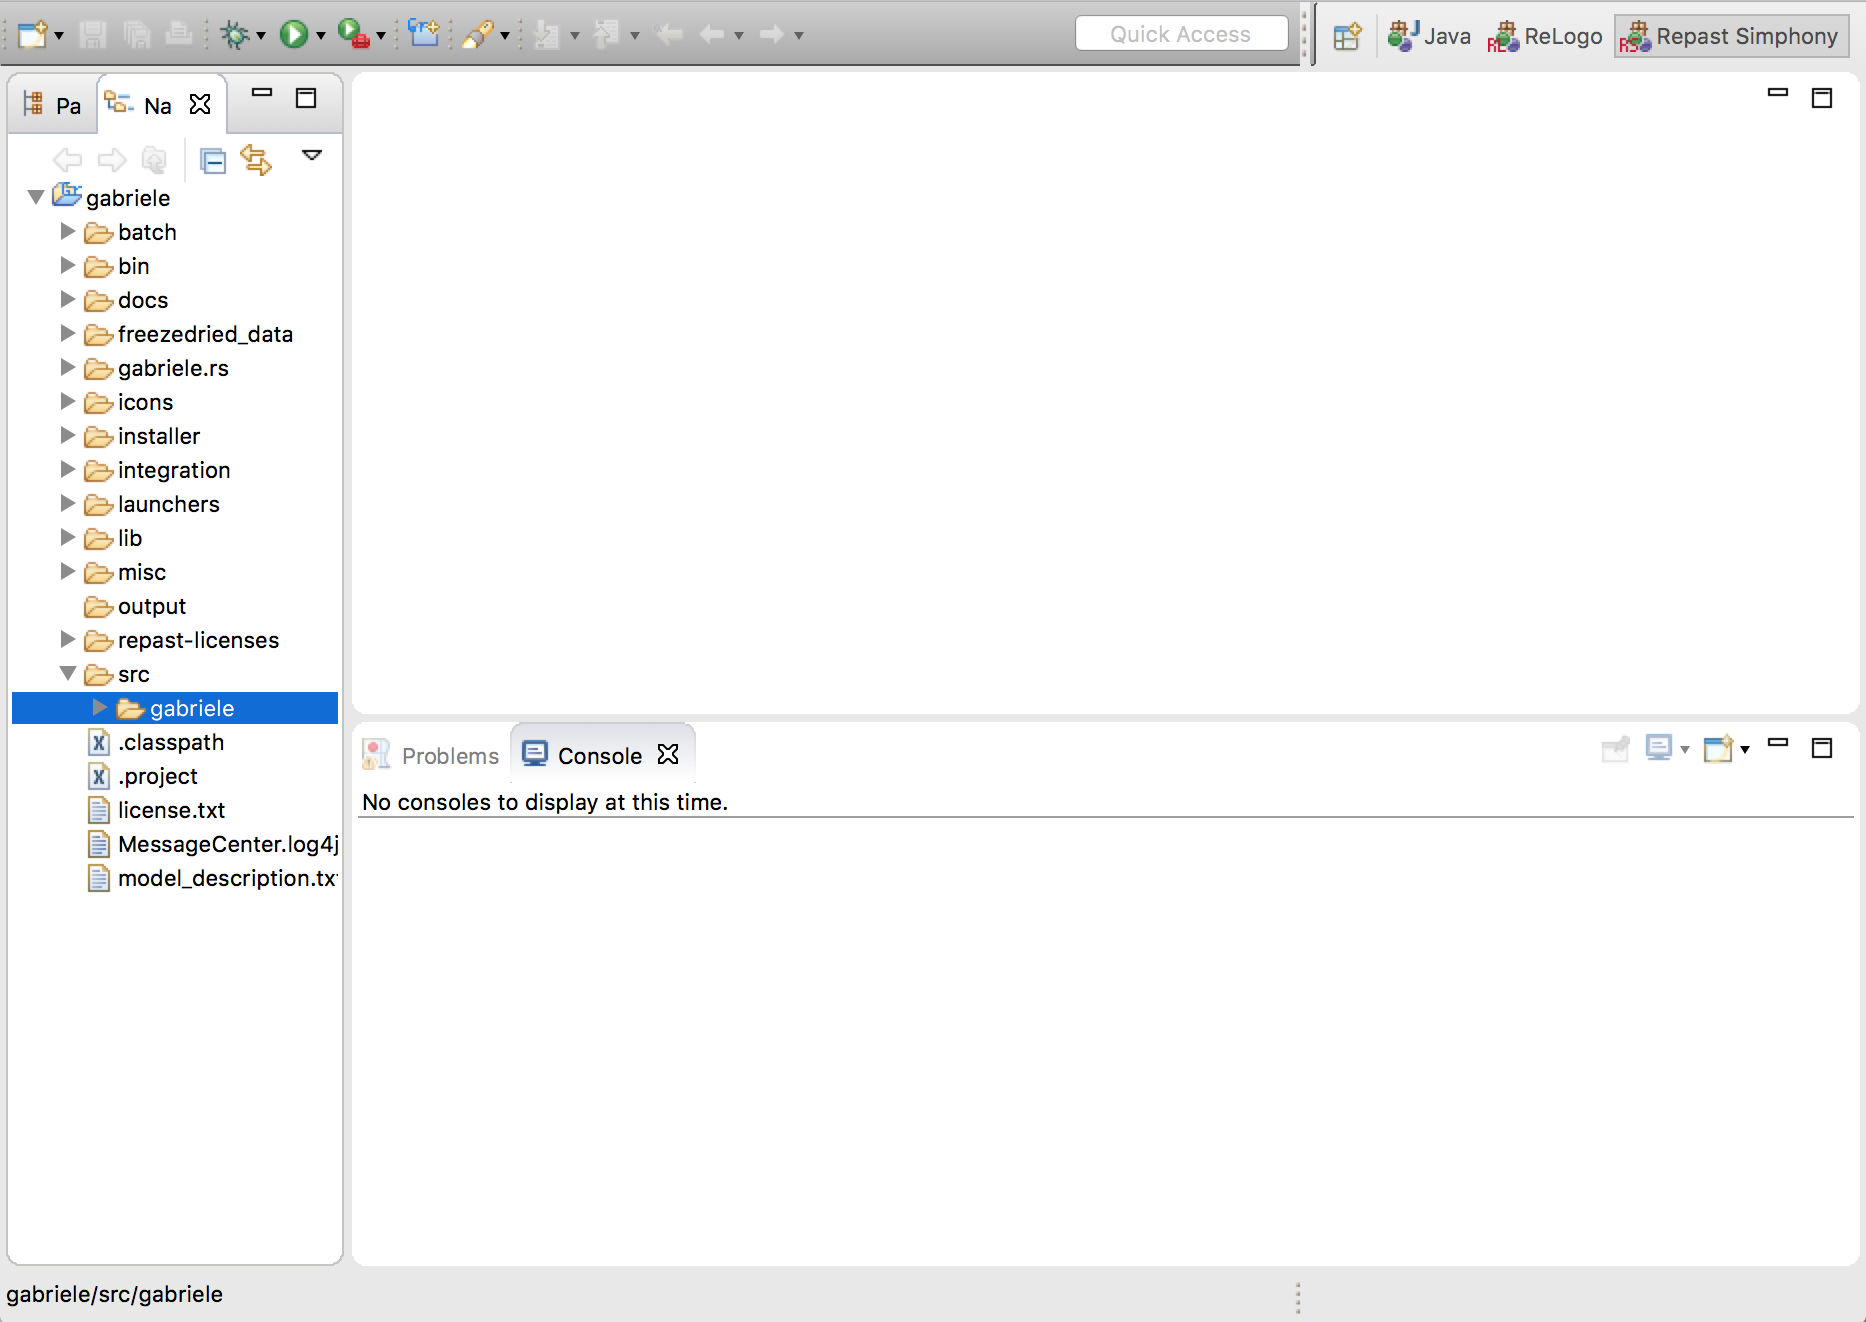
\includegraphics[scale=0.35]{fig_gabriele_rs_navigation}

\iffalse
\begin{verbatim}
/Users/coolcoder/Documents/workspace/gabriele
/Users/coolcoder/Documents/workspace/gabriele/batch
/Users/coolcoder/Documents/workspace/gabriele/bin
. . . 
/Users/coolcoder/Documents/workspace/gabriele/gabriele.rs
. . . 
/Users/coolcoder/Documents/workspace/gabriele/src
/Users/coolcoder/Documents/workspace/gabriele/src/gabriele
\end{verbatim}
\fi
%Now, the source code of the \verb+gabriele+ package and the parameters file have to be added to the gabriele project.

\vskip2mm
Now, the \verb+gabriele+ files have to be added to the just created RS project folders tree.

We give here two alternatives: via git and using a zipped archive.

\subsubsection{Using git}

As you probably know, this is a popular way to share code. % developments you will do.
%So, let us show how to fetch the GABRIELE files via git. To do that, 
To fetch GABRIELE code, a git client need to be installed in your system. Many system comes with a git client already installed; if it is not your case, you have to install it. Mac and windows users can consider to install the GitHub Desktop software.

You can verify if git is installed in your system by checking if your command line interface recognize the \verb+git+ command.  
If your check is successful, change directory to the gabriele project folder:\\
\verb+cd /Users/coolcoder/Documents/workspace/gabriele+\\
and type the following commands:
\begin{verbatim}
git init
git remote add origin https://github.com/ggiulion/gabriele.git
git fetch origin master
git reset --hard FETCH_HEAD
\end{verbatim}

Then if you plan to make your code changes available on GitHub, add the command:\\
\verb+git push --set-upstream origin master+

Now, the gabriele files should show up in the RS project folders.
Refresh the gabriele RS project with the navigation tab selected in the side bar (file $\rightarrow$ refresh) to make them visible in eclipse.

The following figure show how the \verb+src+ sub folder should look like.

\vskip2mm
\noindent
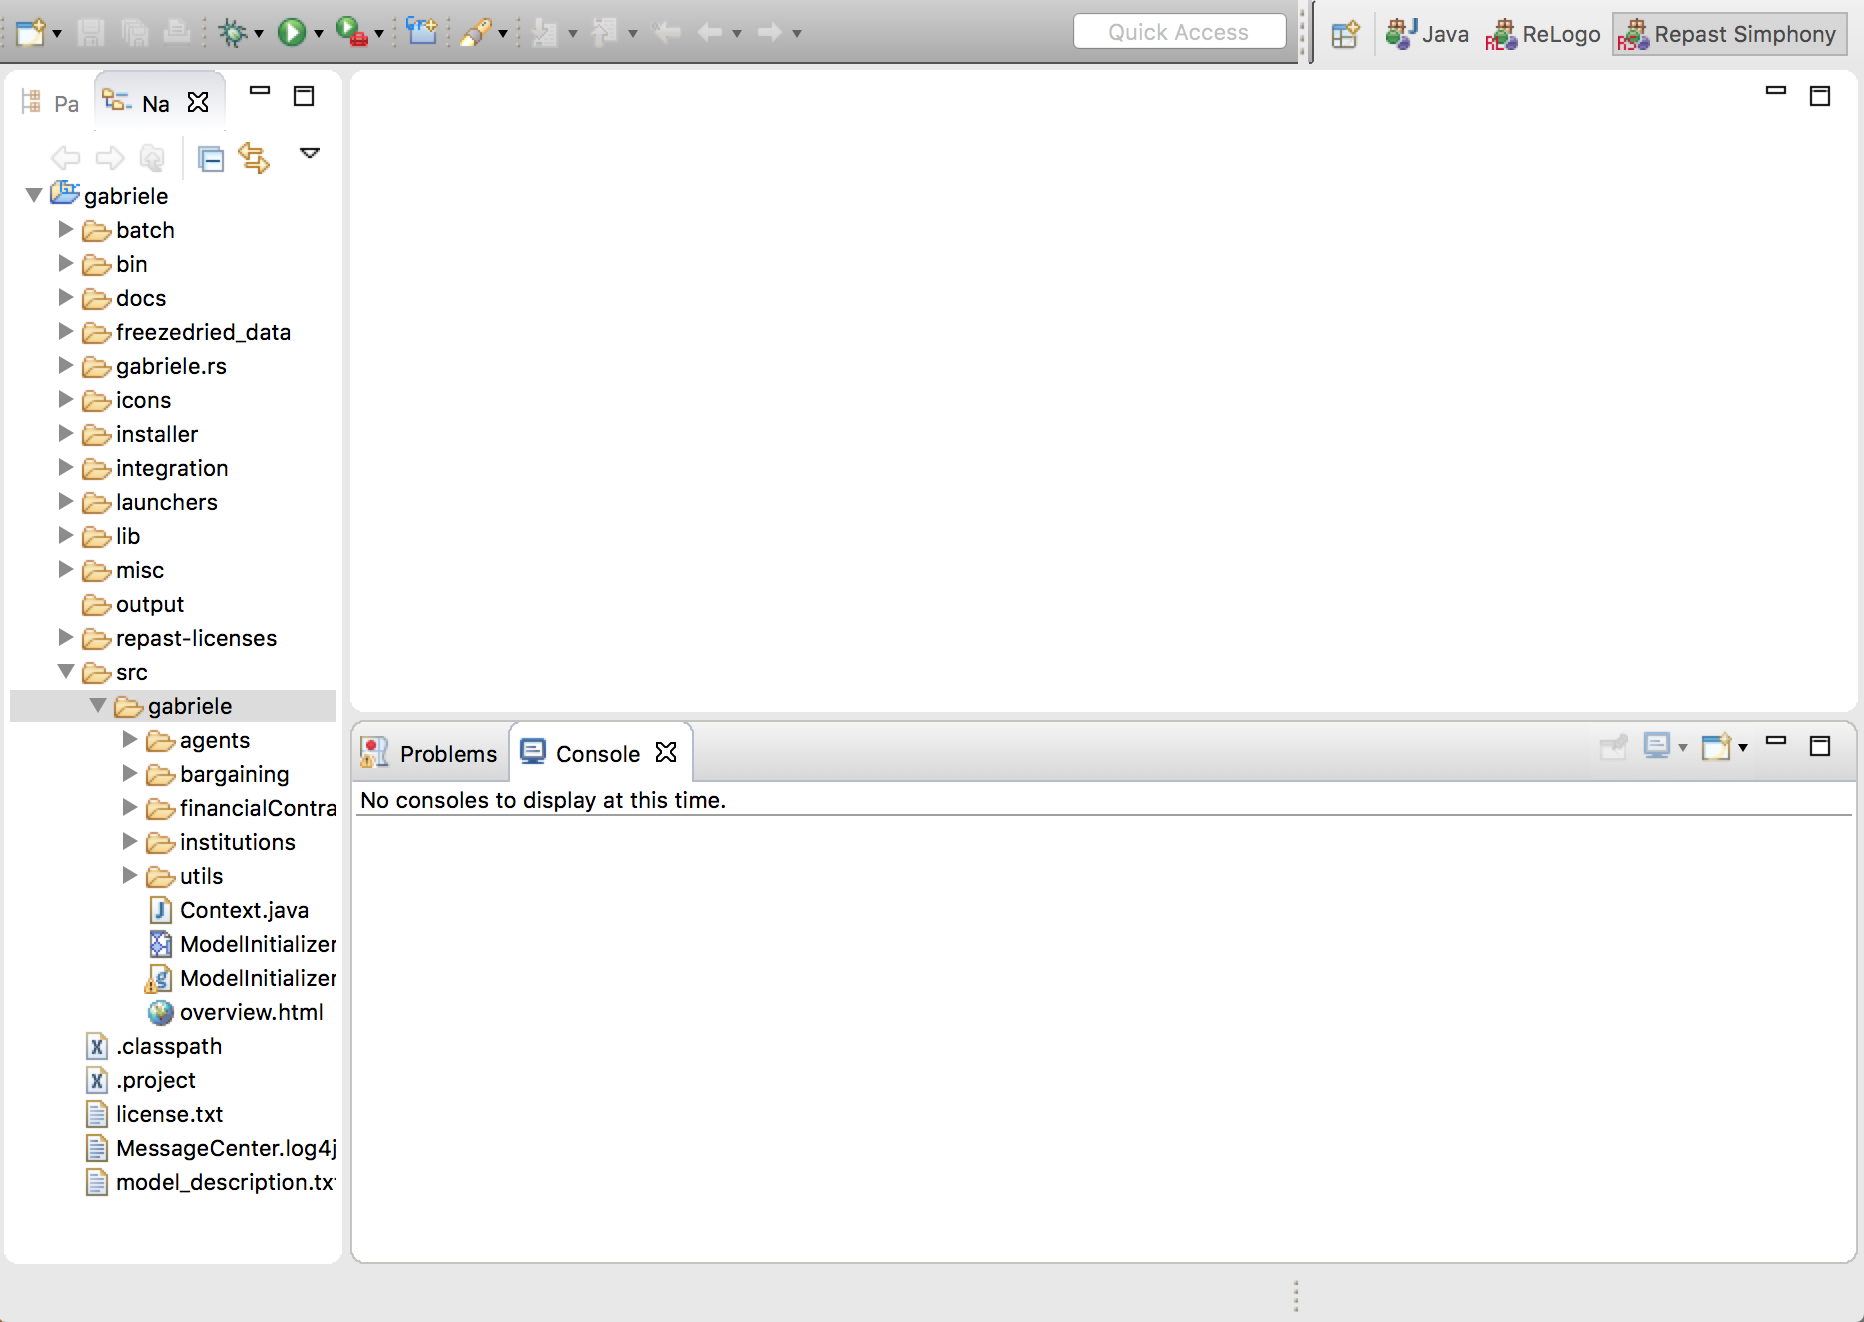
\includegraphics[scale=0.35]{fig_gabriele_rs_navigation1}

\vskip2mm

\subsubsection{Using a zip archive}
Point your browser to\\ 
\verb+https://github.com/ggiulion/gabriele+\\
Click the ``clone or download'' button and choose ``download zip''.

This will download the \verb+gabriele-master.zip+ file in your system.

Unpacking it creates the gabriele-master folder.
Move the whole content of this folder in the gabriele RS project folder:\\  
\verb+/Users/coolcoder/Documents/workspace/gabriele/+\\
Choose to overwrite existing files and folders if you will be asked (this will merge folders). 
\iffalse
At the end of this process one must have

\begin{verbatim}
/Users/coolcoder/Documents/workspace/gabriele/agents/Bank.java
/Users/coolcoder/Documents/workspace/gabriele/agents/Consumer.java
/Users/coolcoder/Documents/workspace/gabriele/agents/Firm.java
/Users/coolcoder/Documents/workspace/gabriele/agents/Industry.java
/Users/coolcoder/Documents/workspace/gabriele/agents/package-info.java
/Users/coolcoder/Documents/workspace/gabriele/bargaining/AProductDemand.java
/Users/coolcoder/Documents/workspace/gabriele/bargaining/Curriculum.java
/Users/coolcoder/Documents/workspace/gabriele/bargaining/LaborOffer.java
/Users/coolcoder/Documents/workspace/gabriele/Context.java
/Users/coolcoder/Documents/workspace/gabriele/financialContracts/BankAccount.java
/Users/coolcoder/Documents/workspace/gabriele/institutions/CentralBank.java
/Users/coolcoder/Documents/workspace/gabriele/institutions/Government.java
/Users/coolcoder/Documents/workspace/gabriele/institutions/LaborMarket.java
/Users/coolcoder/Documents/workspace/gabriele/institutions/OfficeForStatistics.java
/Users/coolcoder/Documents/workspace/gabriele/utils/AbsoluteRankNonAggregateDataSource.java
\end{verbatim}

Finally you have to overwrite the \verb+parameter.xml+ file already present in\\  
\verb+/Users/coolcoder/Documents/workspace/gabriele/gabriele.rs+\\
with that supplied with \verb+gabriele+.
\fi
Now refresh eclipse (file $\rightarrow$ refresh).



\section{Testing the Installation}
\subsection{Setup the data loader}


First you have to start the RS GUI window. To do so, click on the down black arrow highlighted by the red circle in the following picture

\noindent
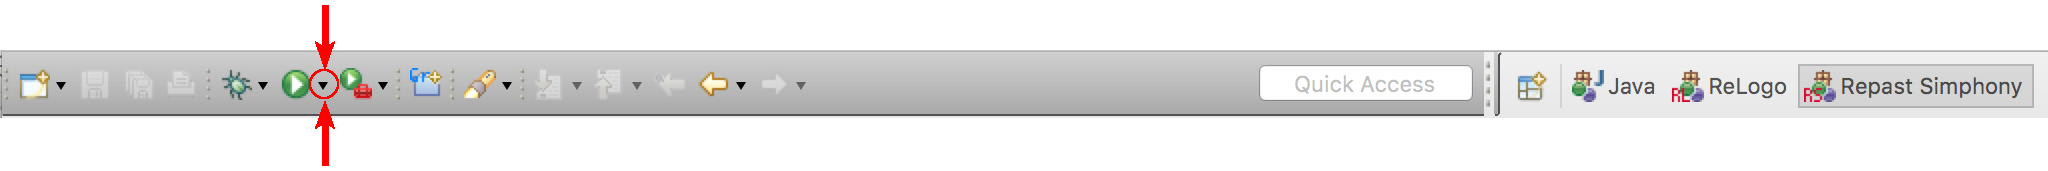
\includegraphics[scale=0.195]{fig_gabriele_rs_execution1a}

After clicking, a menu opens as shown by the following figure. Click the \verb+gabriele Model+ item

\noindent
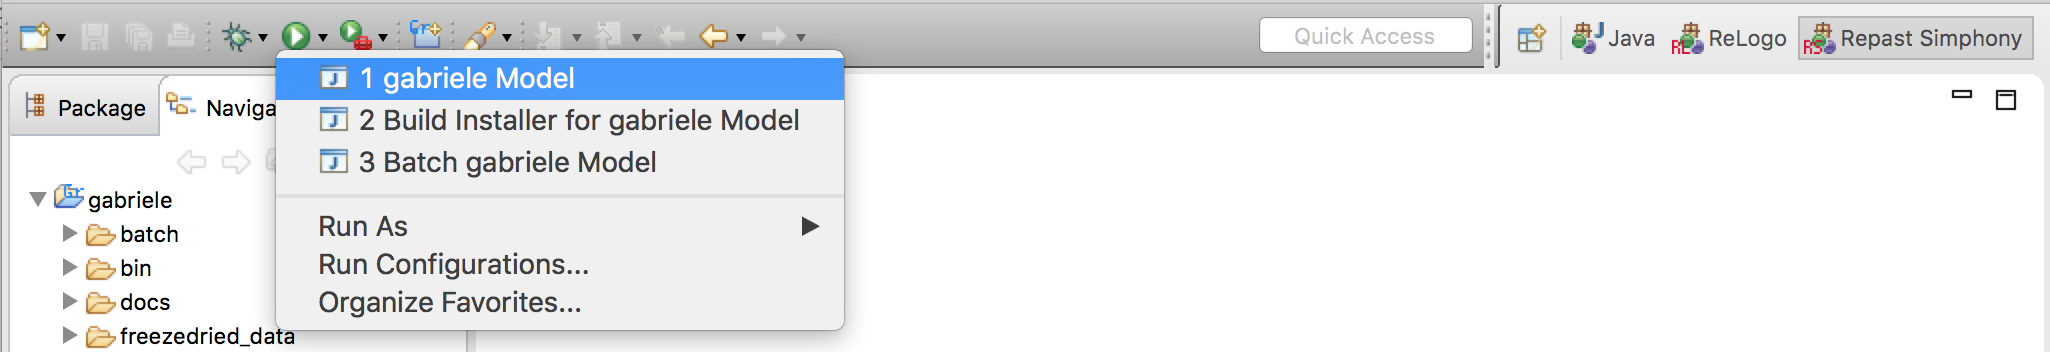
\includegraphics[scale=0.35]{fig_gabriele_rs_execution2}

After a while, the RS GUI (displayed in the following figure) will show up

\noindent
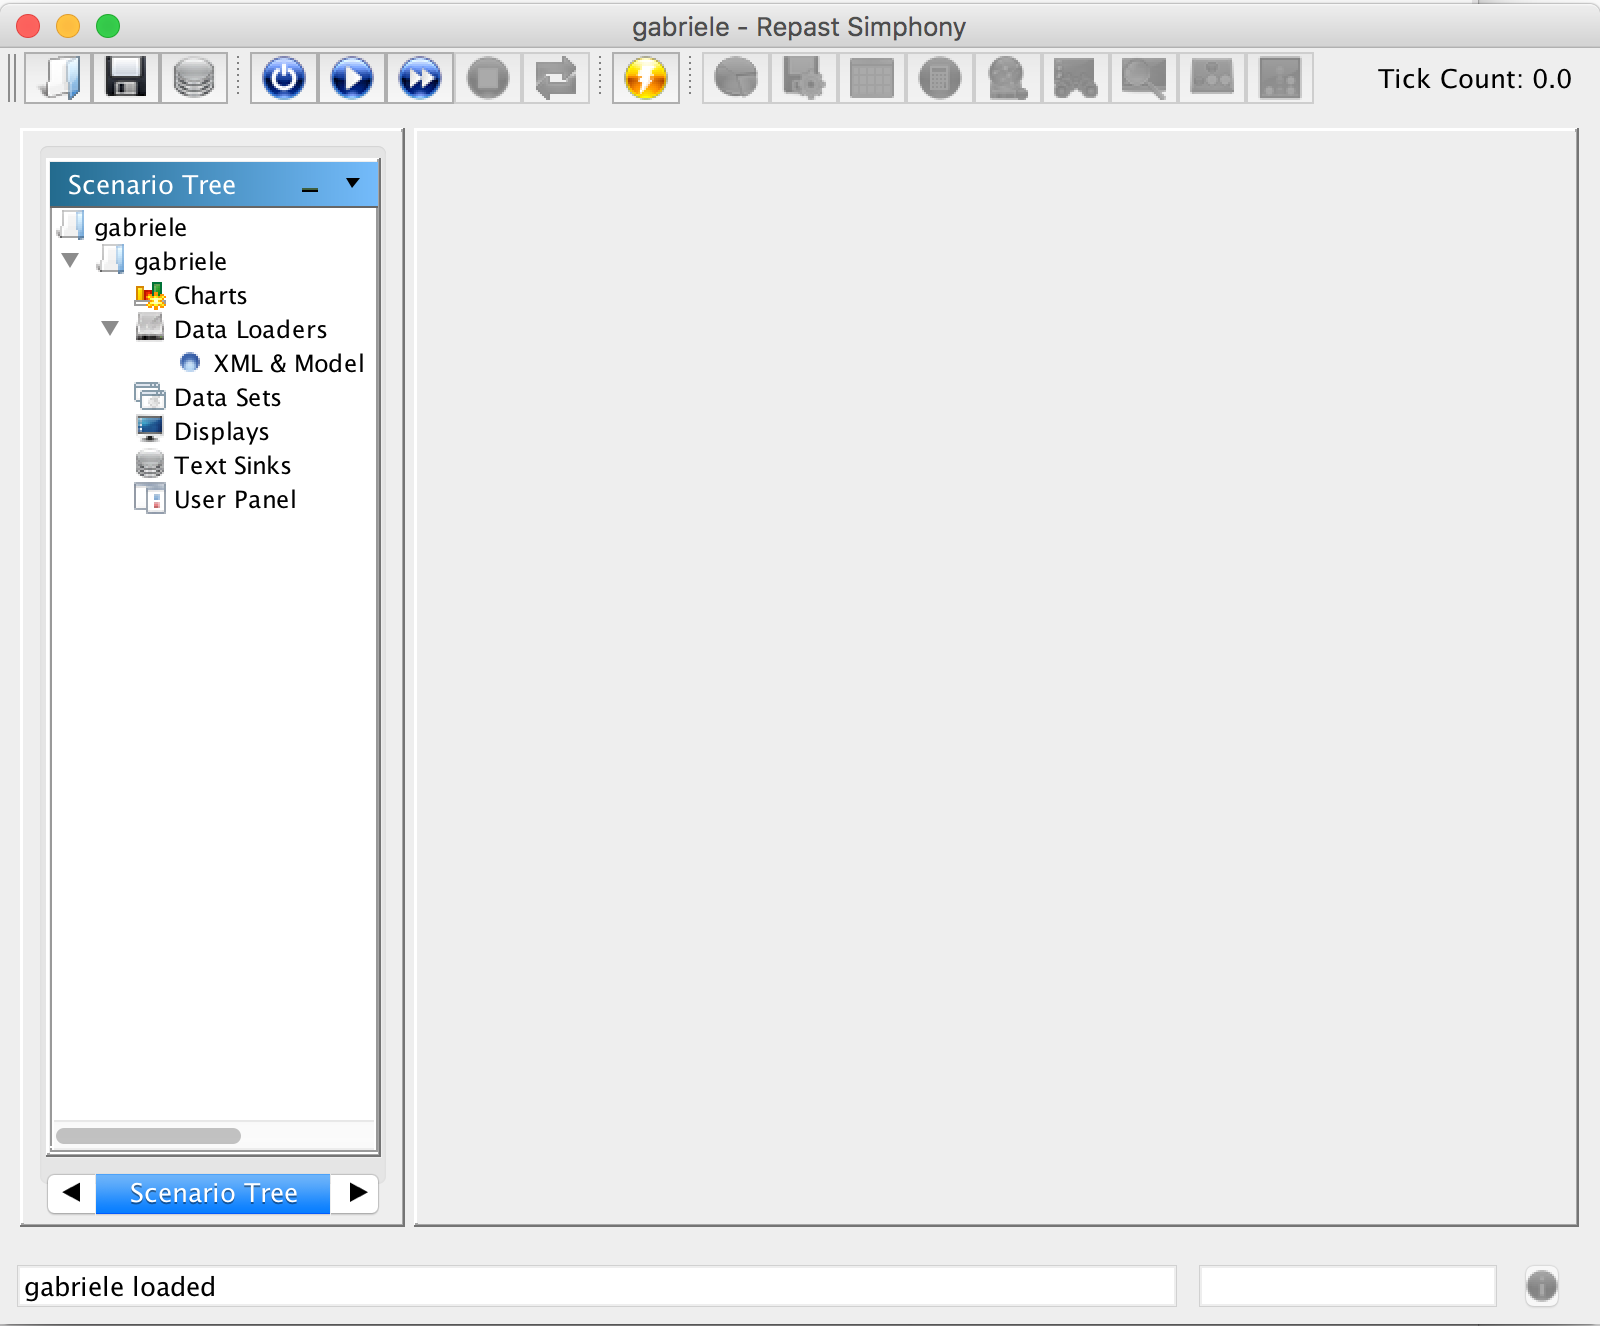
\includegraphics[scale=0.35]{fig_gabriele_rs_gui1}

The first time you start the RS GUI % with the GABRIELE scenario 
you have to setup the custom dataloader. As you can see in the scenario tree under the Data Loaders item, the XML \& Model data loader is present. This must be changed in the custom loader for this model. To do so right click on the Data loaders item and choose set Data Loader as shown in the following figures


\noindent
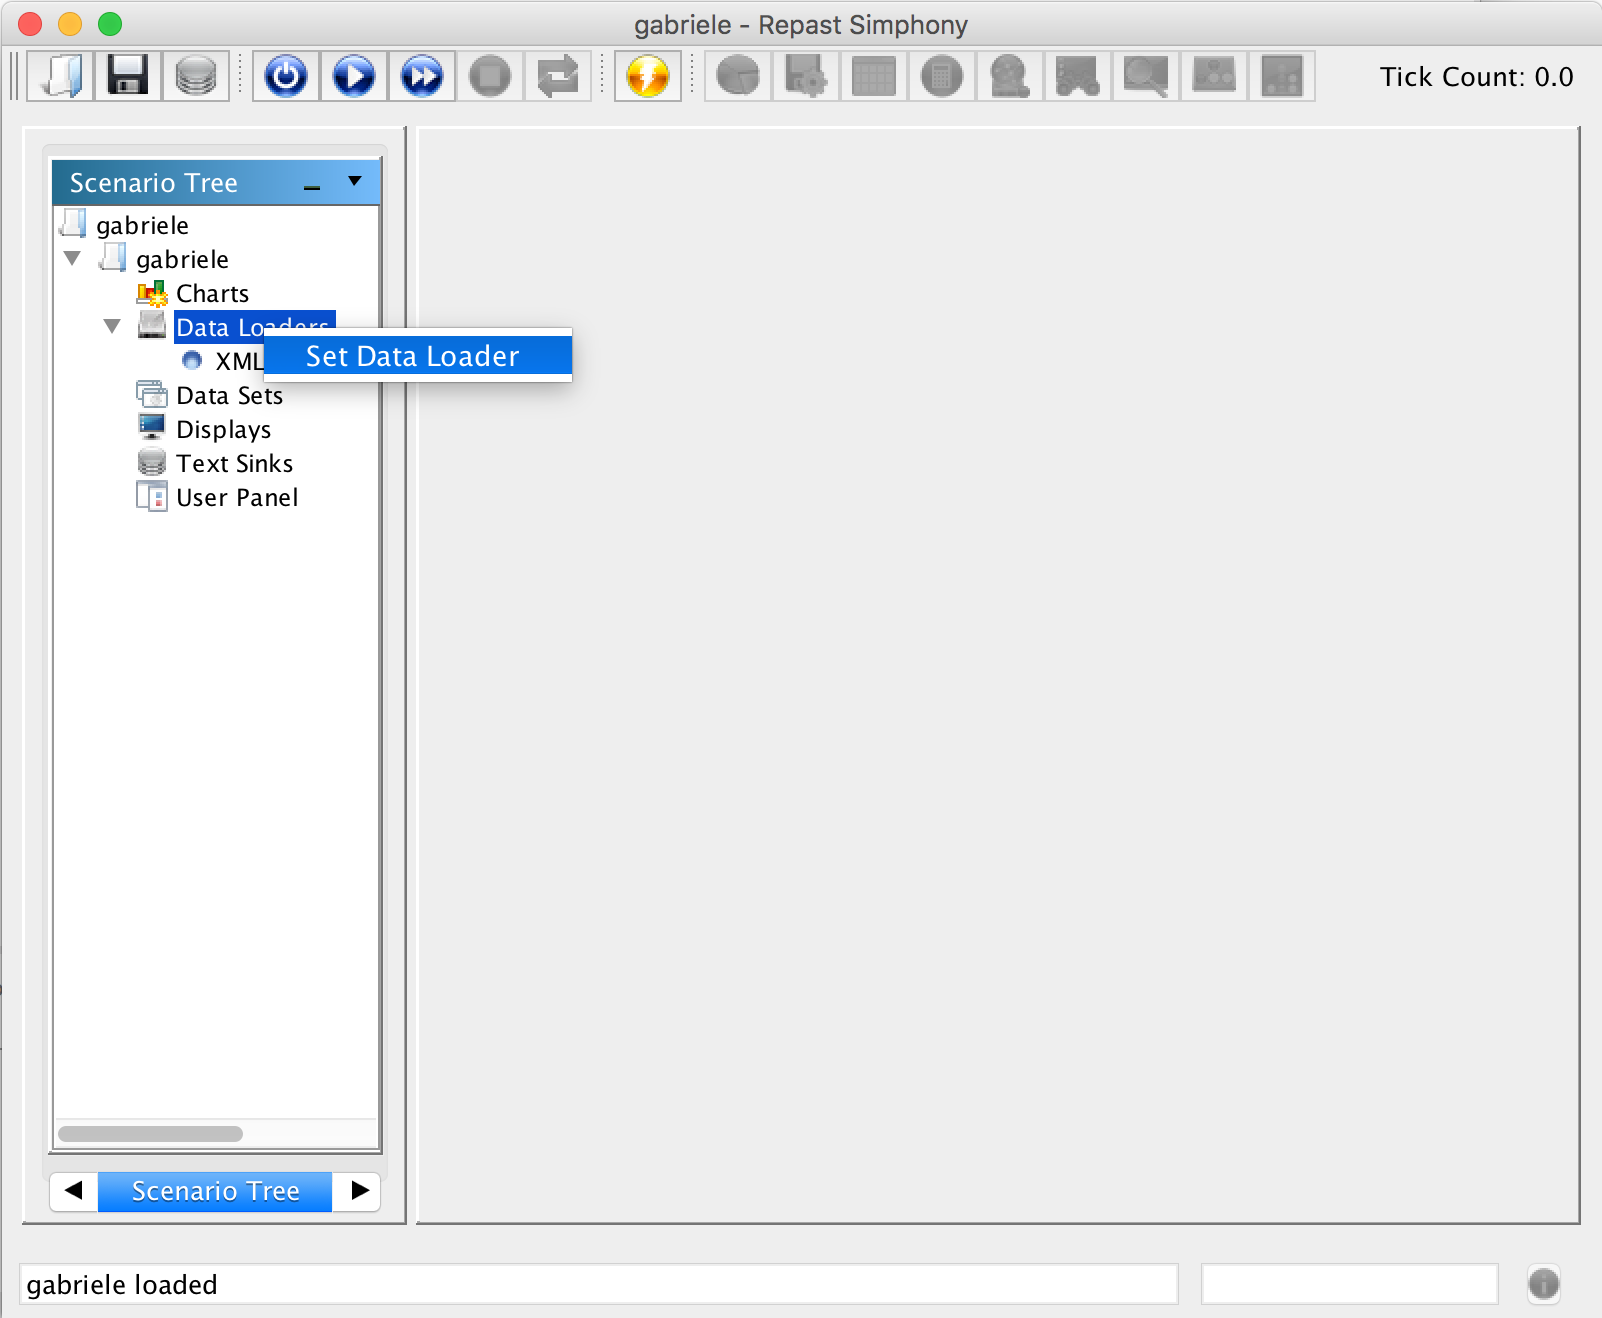
\includegraphics[scale=0.35]{fig_gabriele_rs_gui2}

The following new window will appear

\noindent
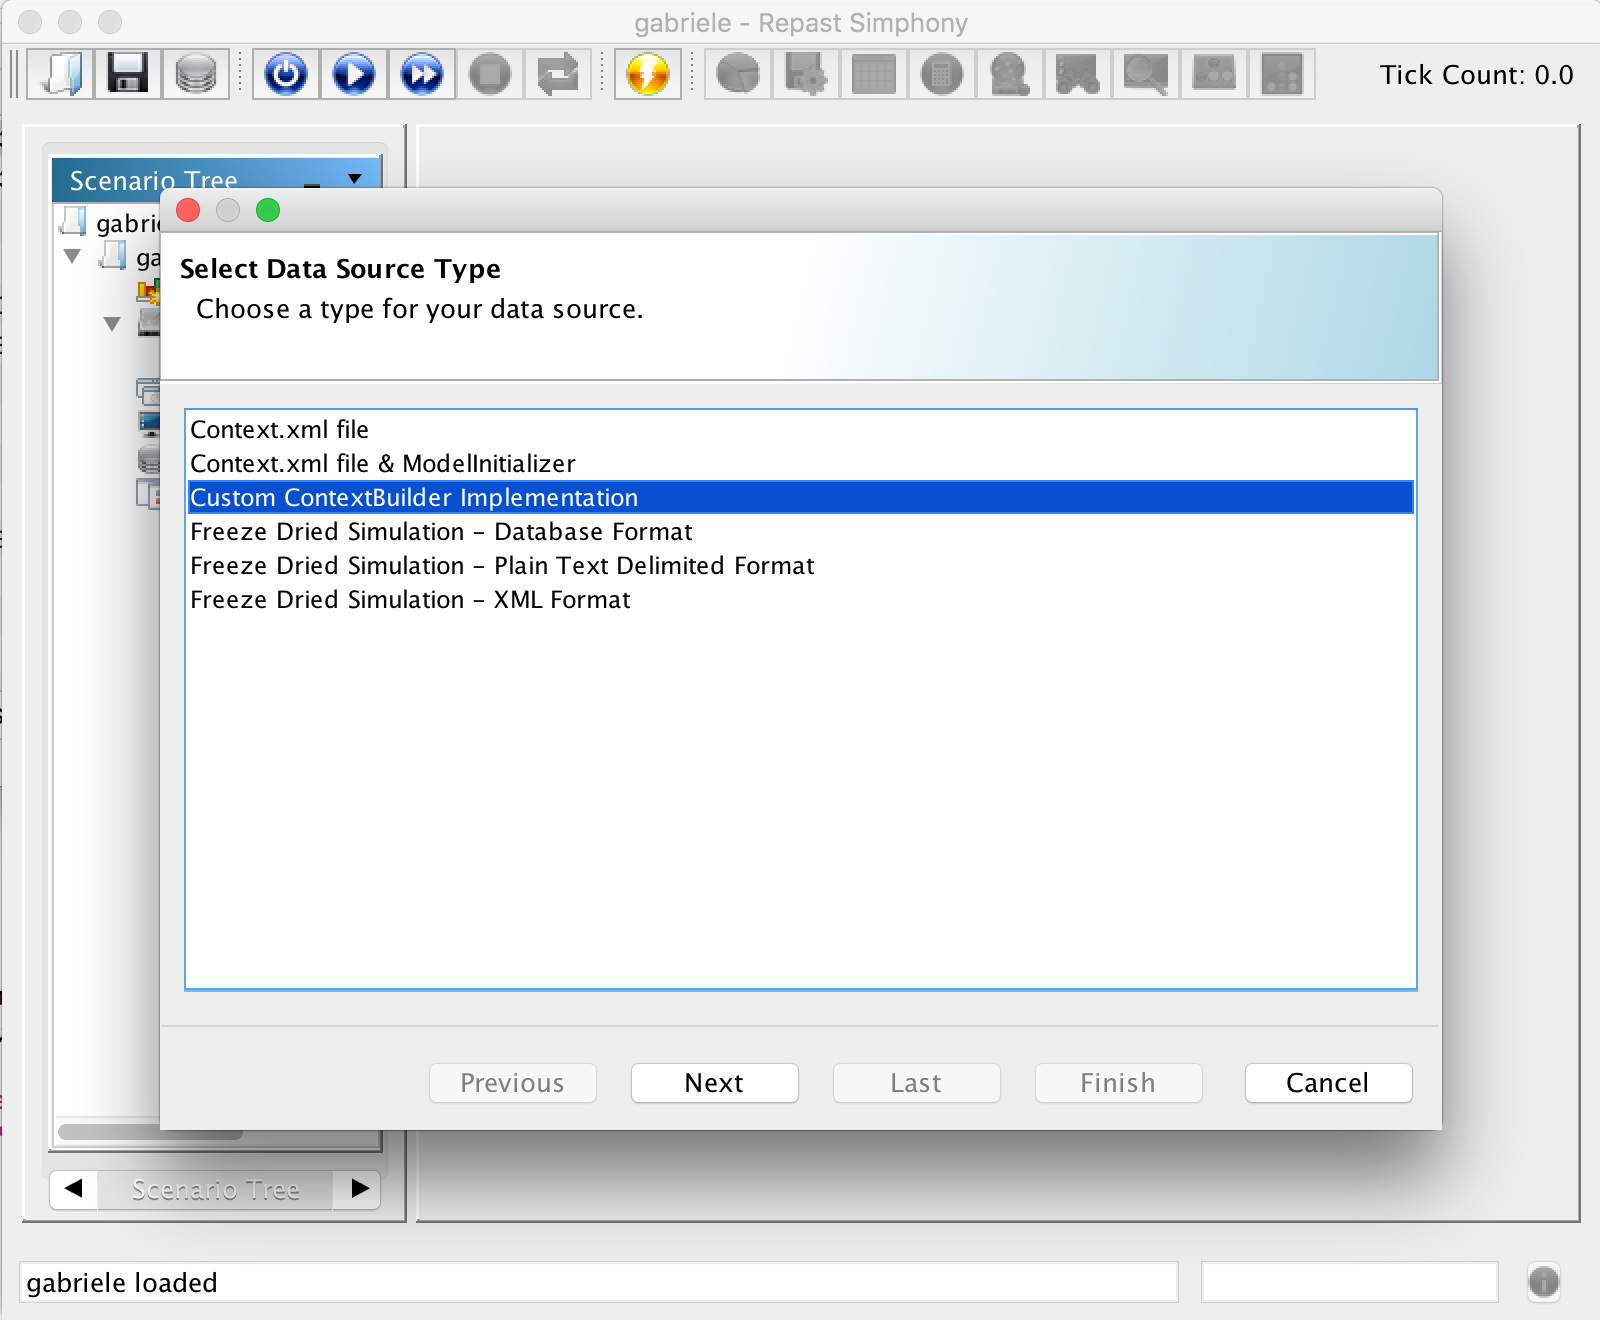
\includegraphics[scale=0.35]{fig_gabriele_rs_gui3}

Choose Custom ContextBuilder implementation and click next:
A new window with a proposal will appear. 

\noindent
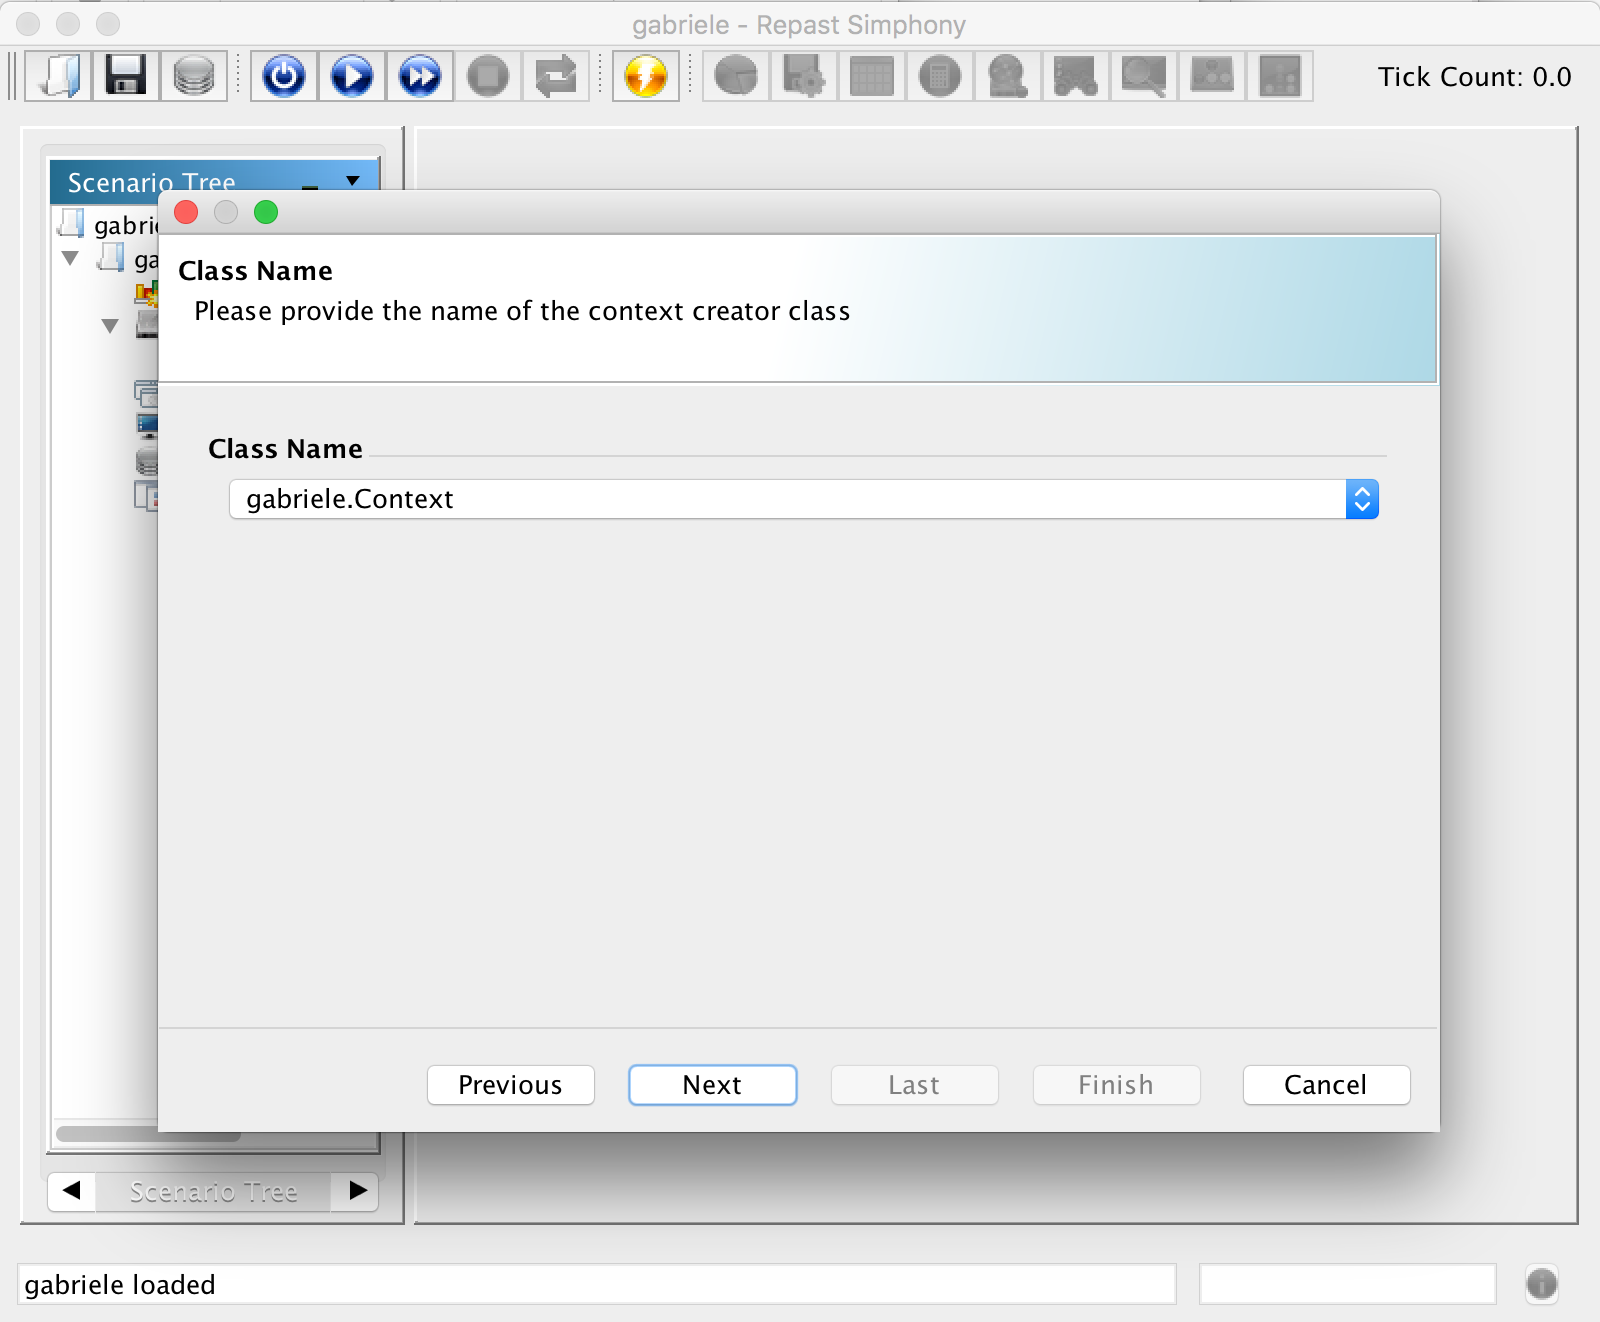
\includegraphics[scale=0.35]{fig_gabriele_rs_gui4}

Clicking next will change the window as follows 

\noindent
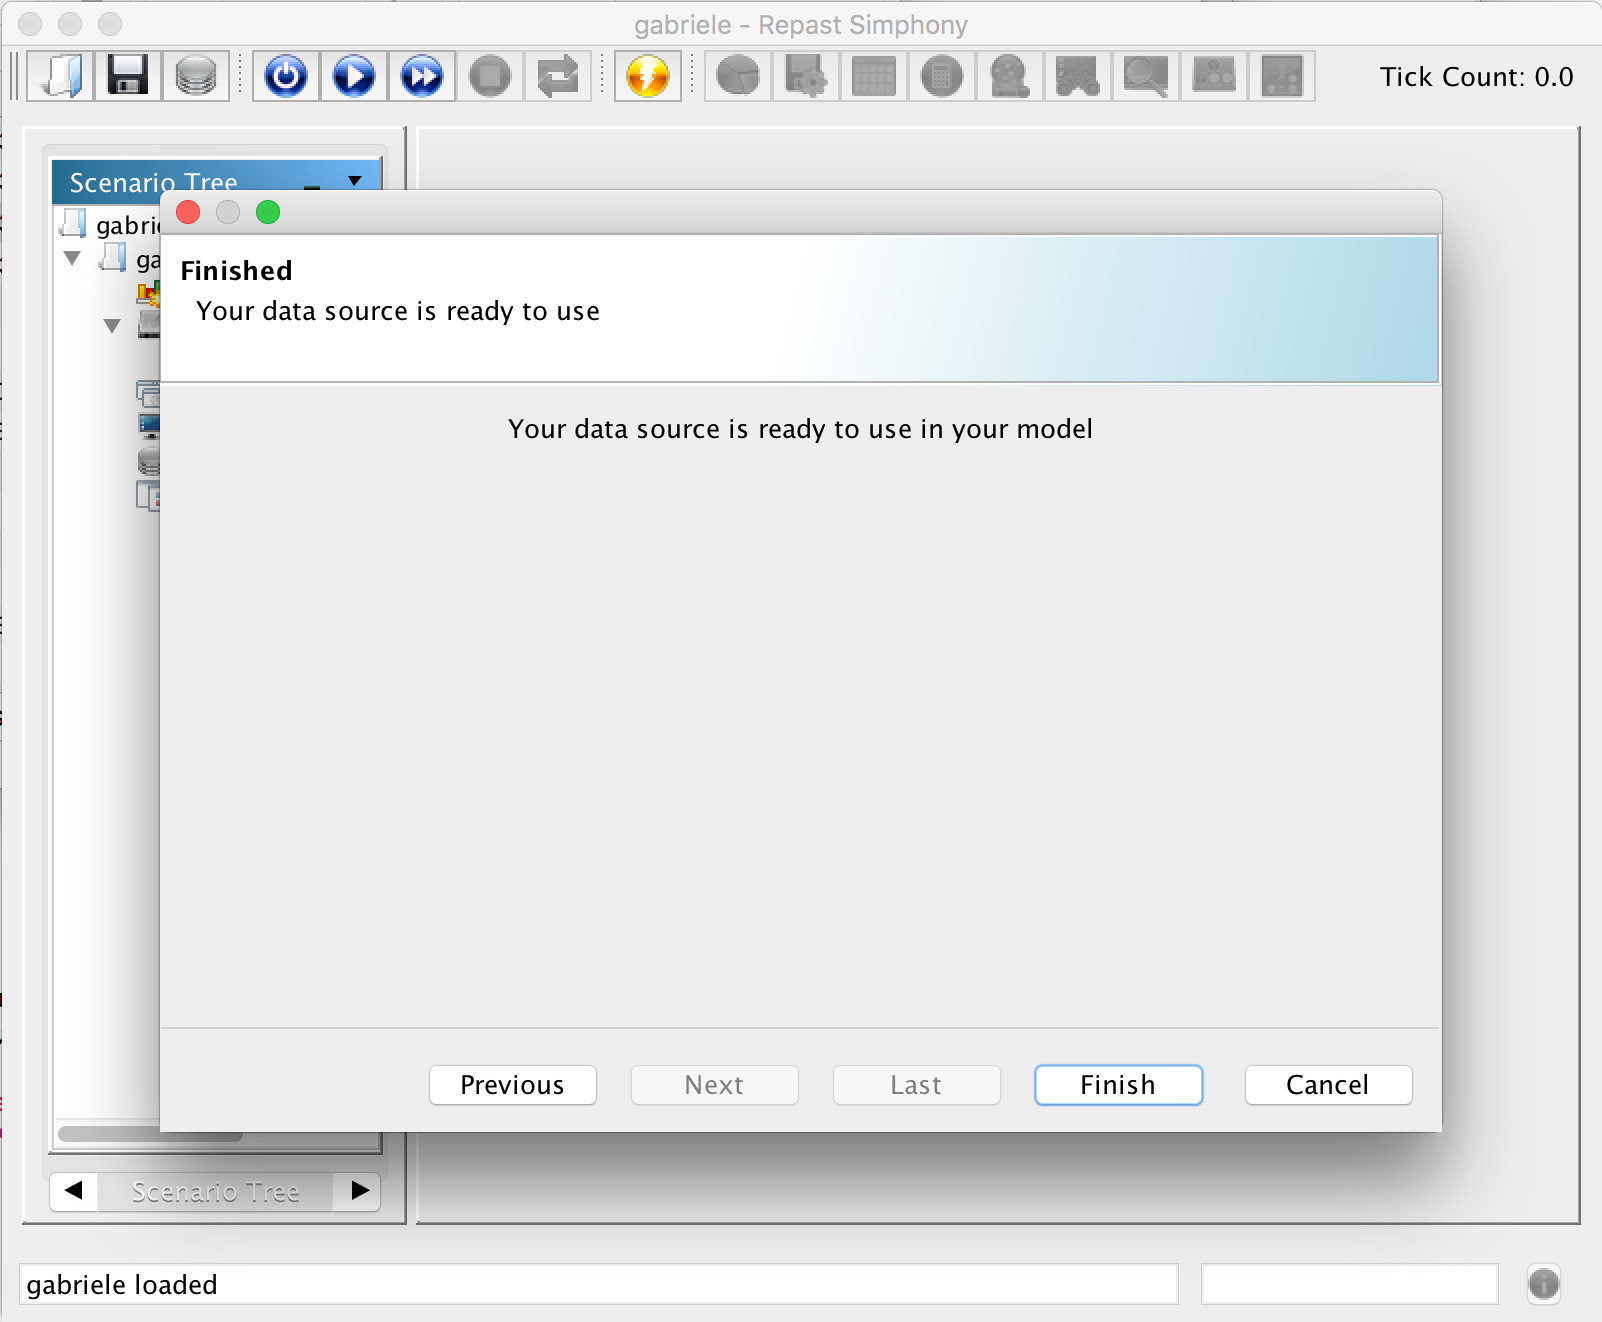
\includegraphics[scale=0.35]{fig_gabriele_rs_gui5}

Click finish.

Now, the previous data loader is replaced by the GABRIELE data loader (Context) as shown by the following figure

\noindent
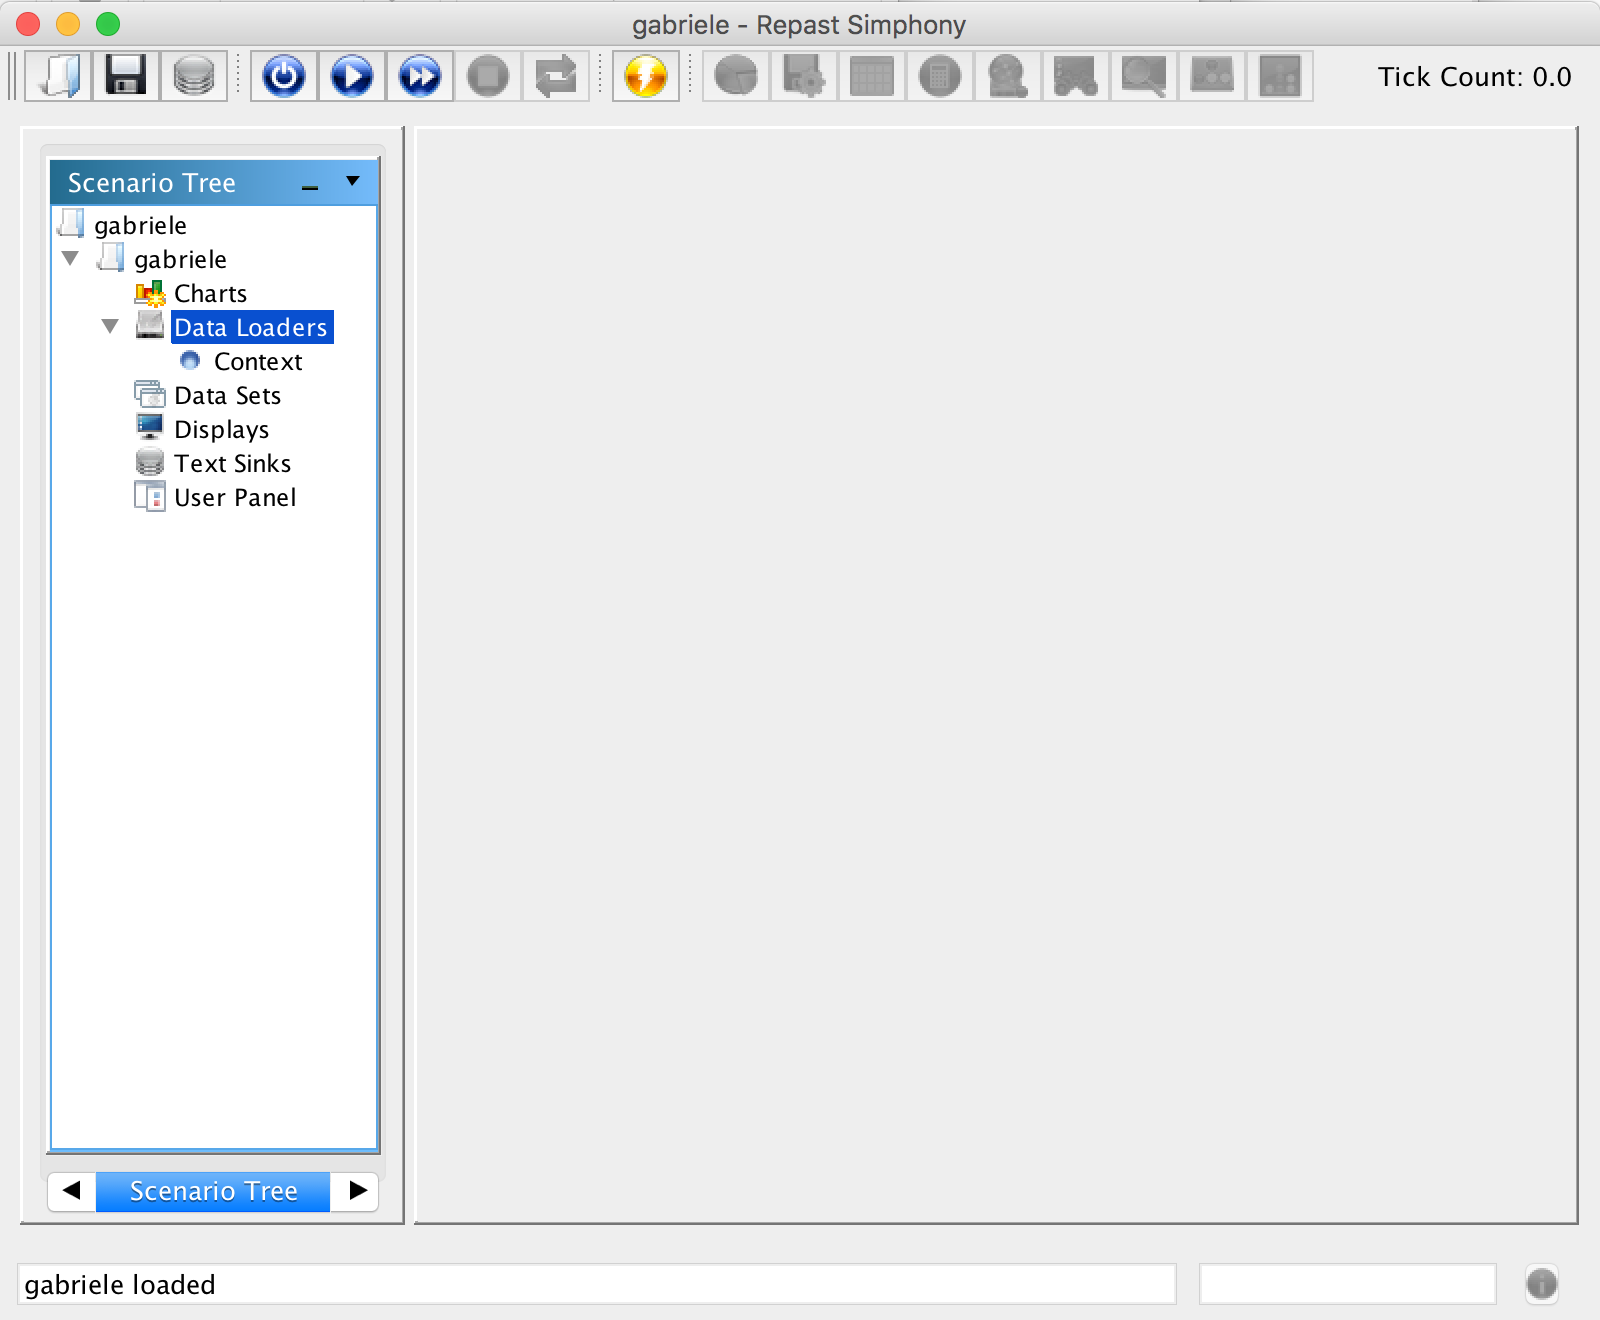
\includegraphics[scale=0.35]{fig_gabriele_rs_gui6}

Click on the floppy disk icon to make the change permanent.

%Now, closing the window you are asked to make your change permanent: 

%\noindent
%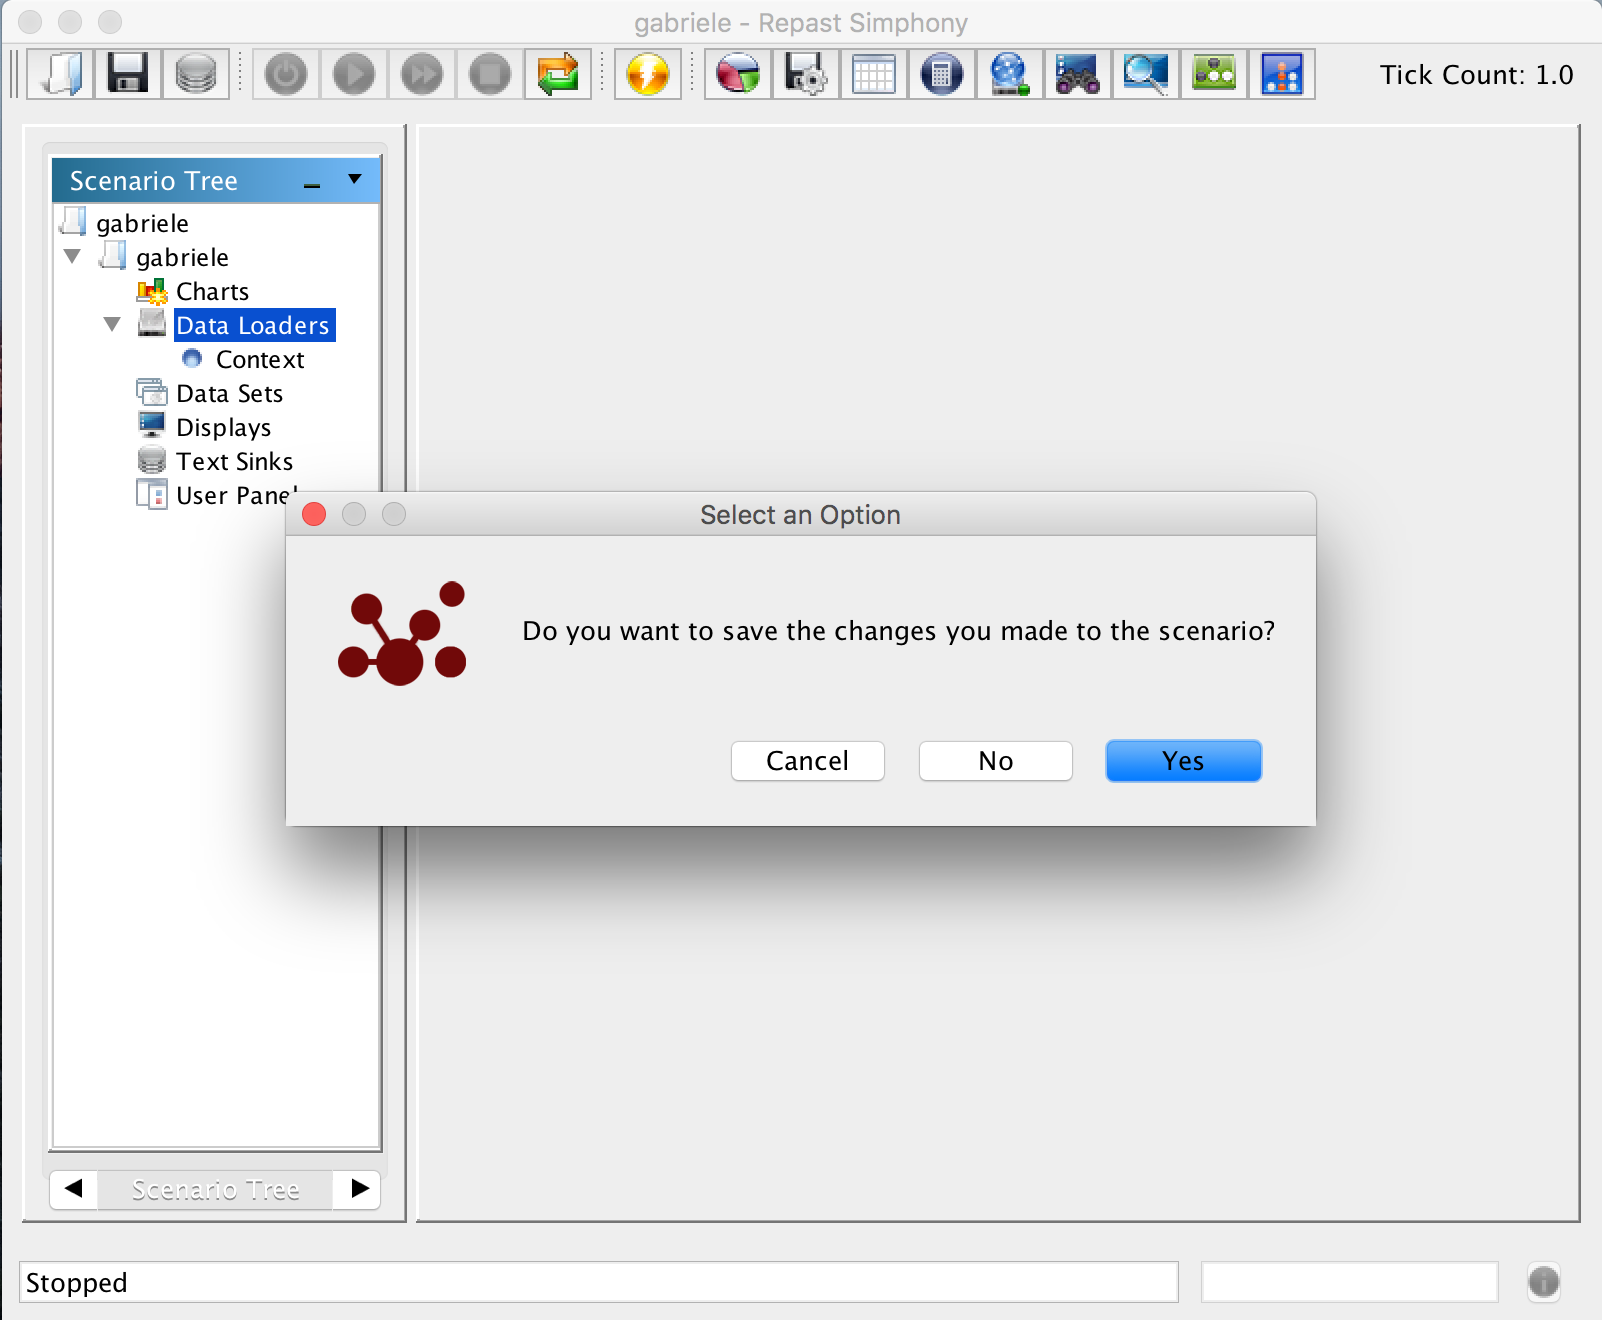
\includegraphics[scale=0.35]{fig_gabriele_rs_gui8}

%Click on yes.

\subsection{Running GABRIELE}


There are two ways of running RS models: The GUI and the BATCH mode.

The GUI mode can be of great visual impact because several monitoring devices continuously updating during the run can be added to the RS GUI window. The flip side of the coin is that these devices slow down simulation execution. Second, the simulation runs exclusively in a machine running an X server. Notwithstanding the GUI mode can be a valid tool during the model development. When massive simulations are performed, the BATCH mode should be used instead. BATCH mode runs are faster because all the graphics elements are turned off. Furthermore, the absence of graphics makes it possible to run the model in parallel on several machines. It is worth saying that RS has very useful facilities for running a model in parallel.


Let us start this section from the very beginning i.e. with the eclipse software just opened and show how to run the model both in GUI and BATCH mode.

First of all, click on the down black arrow highlighted by the red circle in the following picture

\vskip2mm
\noindent
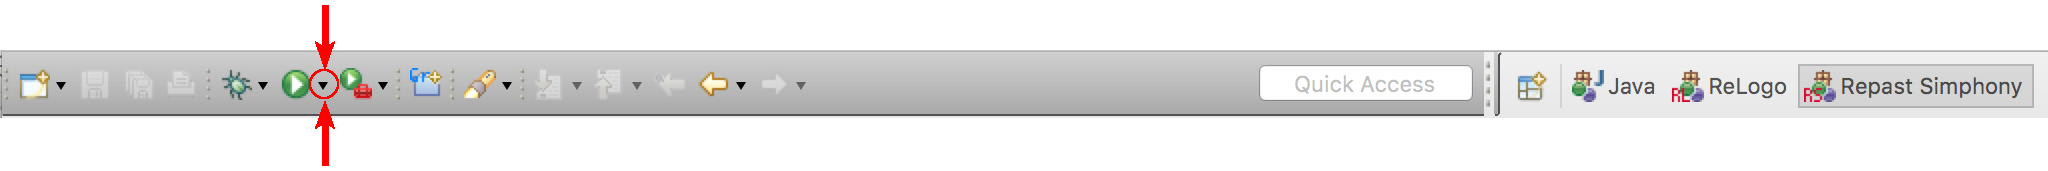
\includegraphics[scale=0.195]{fig_gabriele_rs_execution1a}

After clicking, a menu opens as shown by the following figure. 

\vskip2mm
\noindent
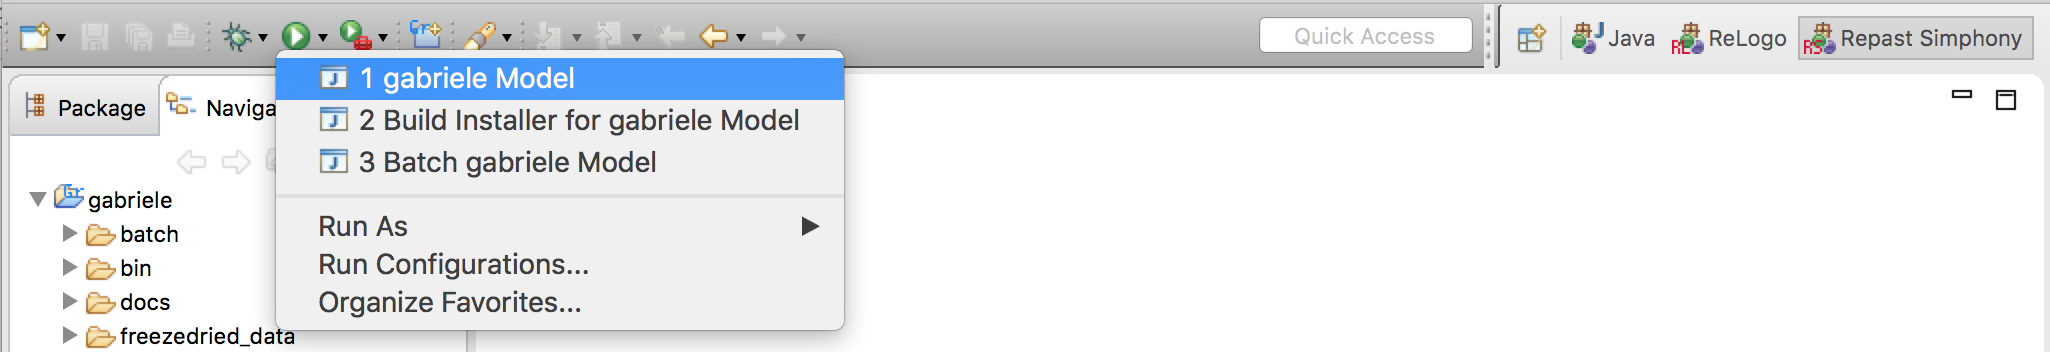
\includegraphics[scale=0.35]{fig_gabriele_rs_execution2}

\vskip2mm
The GUI execution is activated by clicking the \verb+gabriele Model+ item, while the BATCH execution can be started by clicking the \verb+Batch gabriele model+.


\subsubsection{Running in GUI mode}

RS GUI window opens by clicking the \verb+gabriele Model+ item. Check if Context is listed under the Data Loaders item of the scenario tree.

Use the RS GUI window intuitive buttons to interact with the simulation. A more detailed description on how to control the simulation is given at page 24 ``Repast Java Getting Started'' document available in RS web site.

The current version of the model has no runtime monitoring graphical element, so one can check the progress of the simulation watching at the tick count number in upper right corner of the RS GUI window or looking at the text output in the console panel of Eclipse window as shown in the following figure. 

\vskip2mm
\noindent
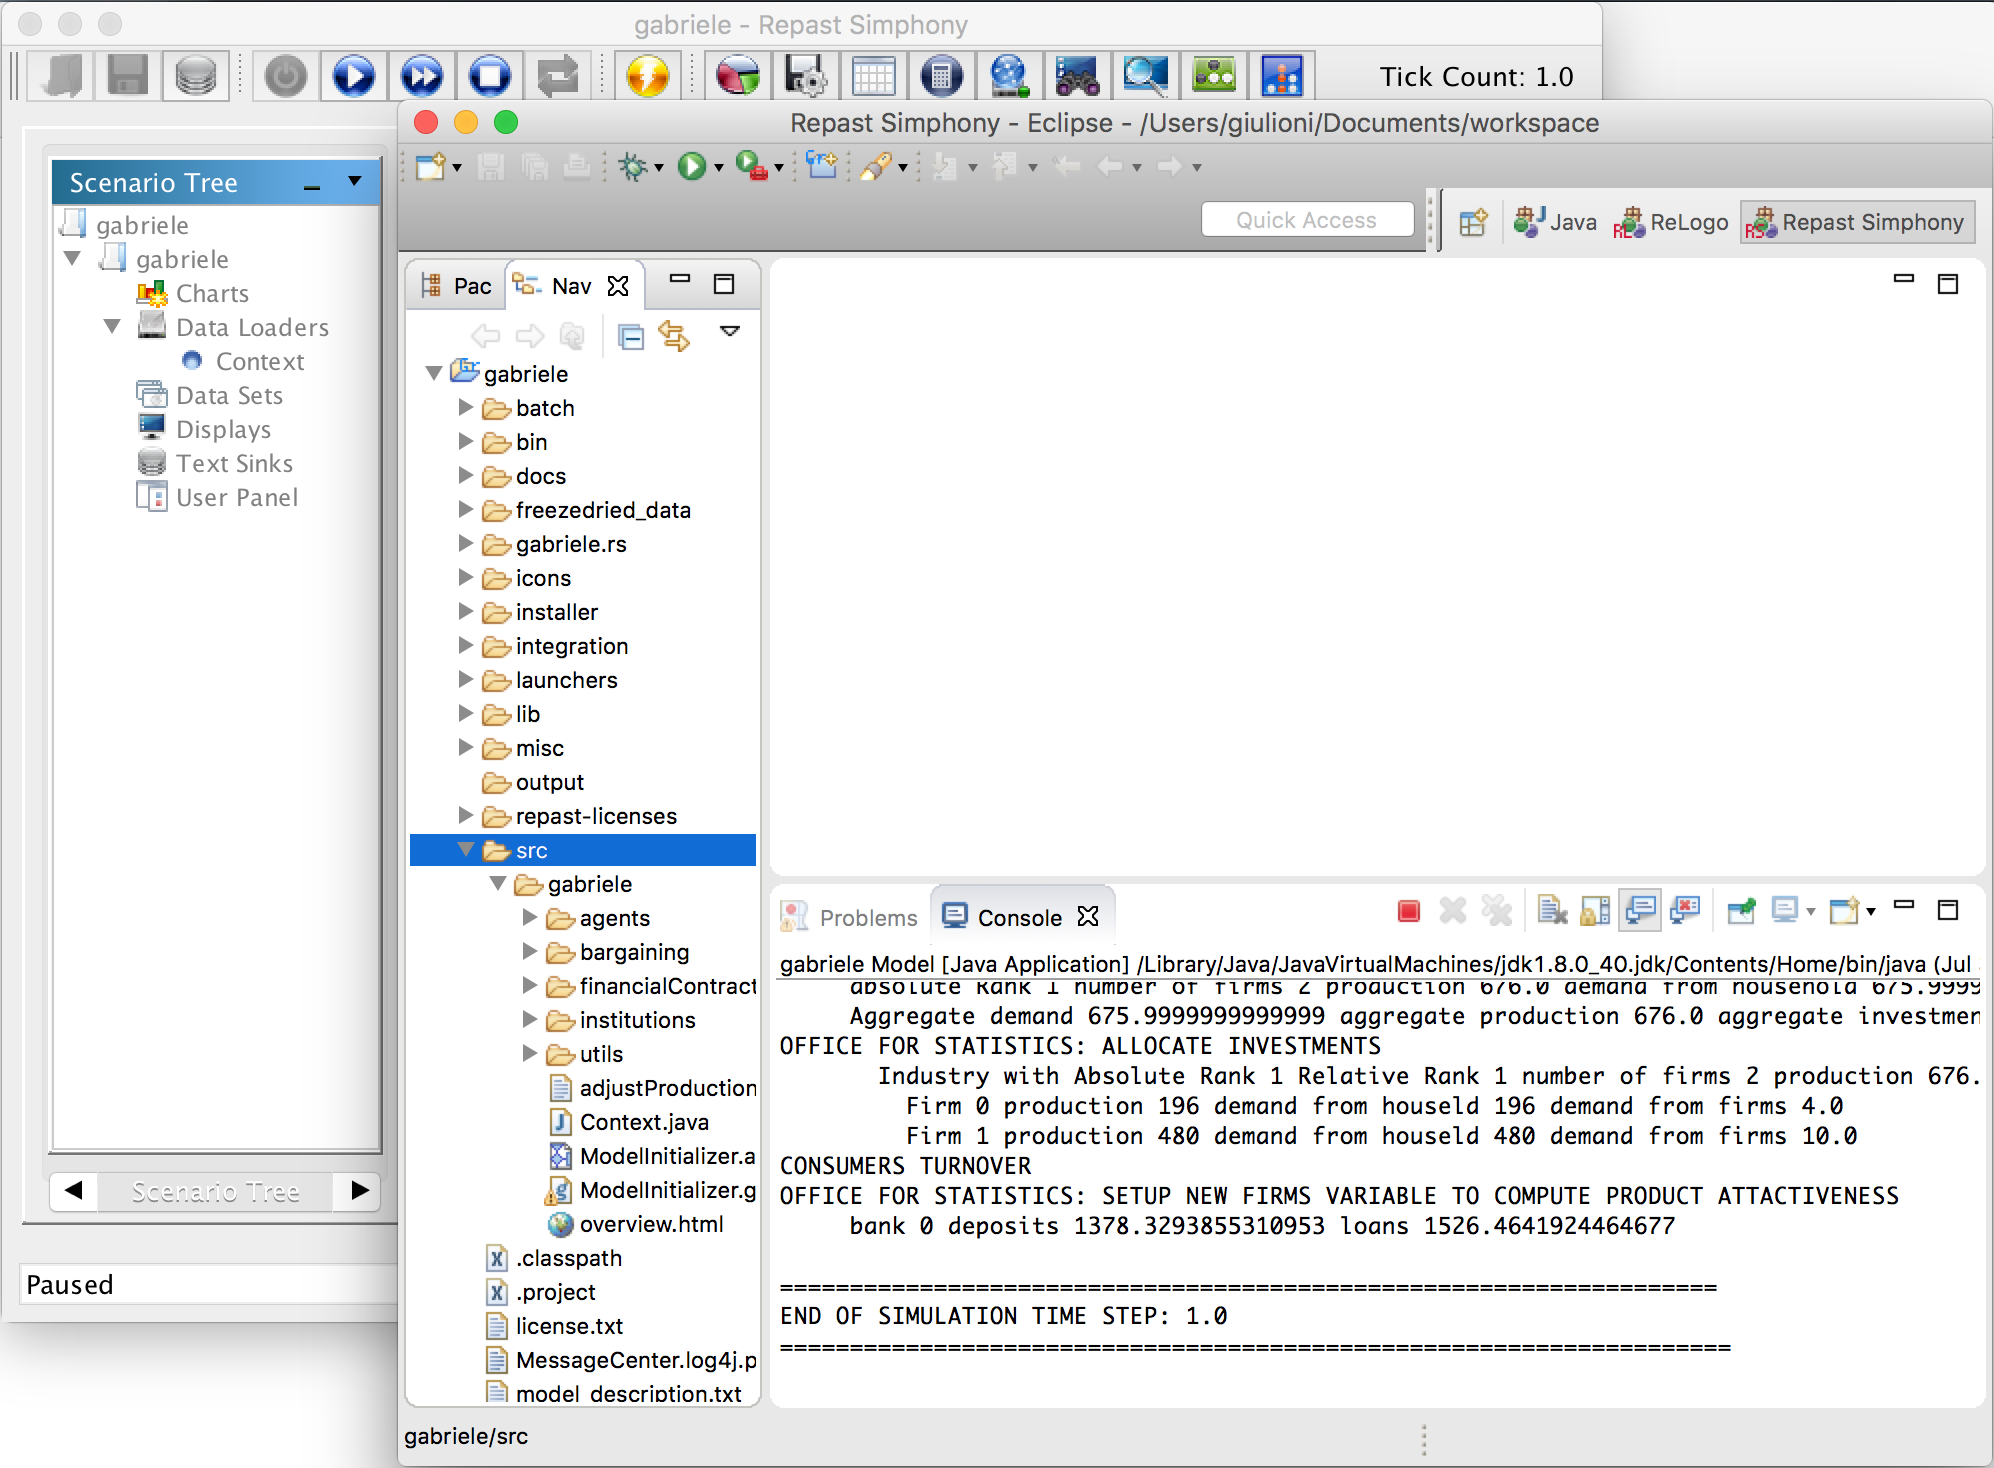
\includegraphics[scale=0.35]{fig_gabriele_rs_gui7}

\vskip2mm
On the other hand, GABRIELE record data in text and csv files that will be created in the model base directory:\\
\verb+/Users/coolcoder/Documents/workspace/gabriele+\\
Data files can be easily identified because their name starts with \verb+zdata+.

The file \verb+zdata_aaa_readme.txt+ gives a description of the contents of all the data files.

\subsubsection{Running in BATCH mode}

Clicking on the \verb+Batch gabriele model+ as in the following figure

\noindent
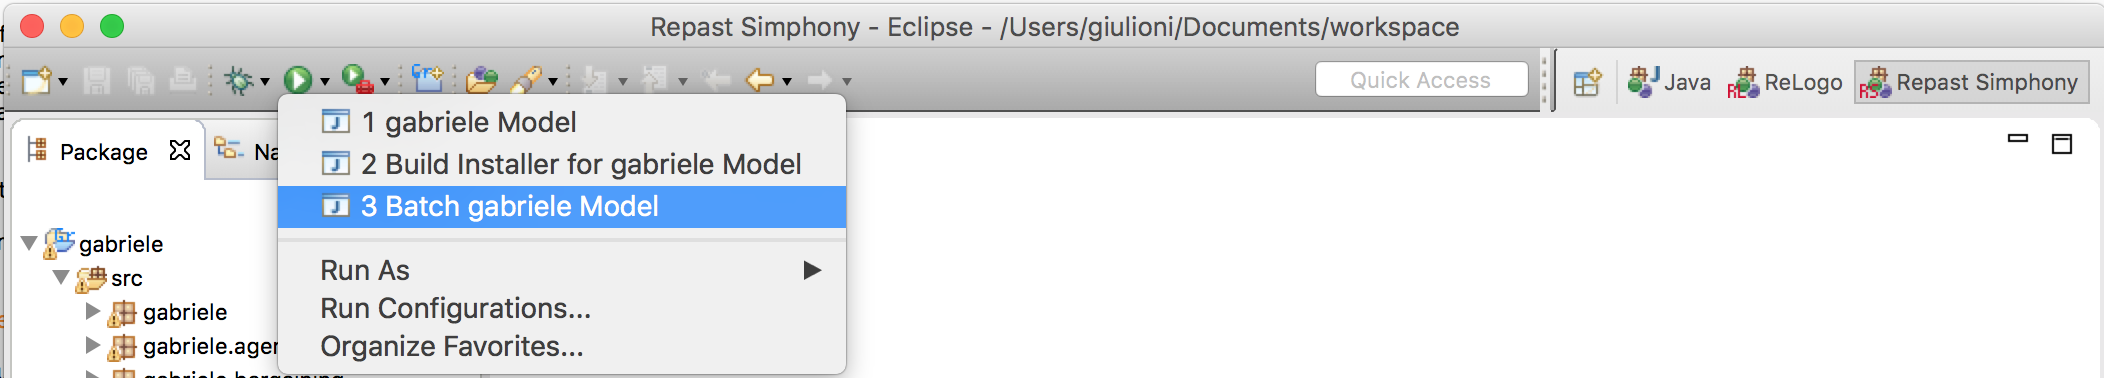
\includegraphics[scale=0.35]{fig_gabriele_rs_execution3}

activates the batch run configuration wizard.

We point the reader to the ``Repast Simphony Batch Runs Getting Started'' document available in RS website for a full description of the wizard.

We only point out that the present version of the model uses custom output recording techniques. Therefore, the RS File Sink are not used. This implies that the ``Optional Output File Patterns'' must be set as in the following figure

\noindent
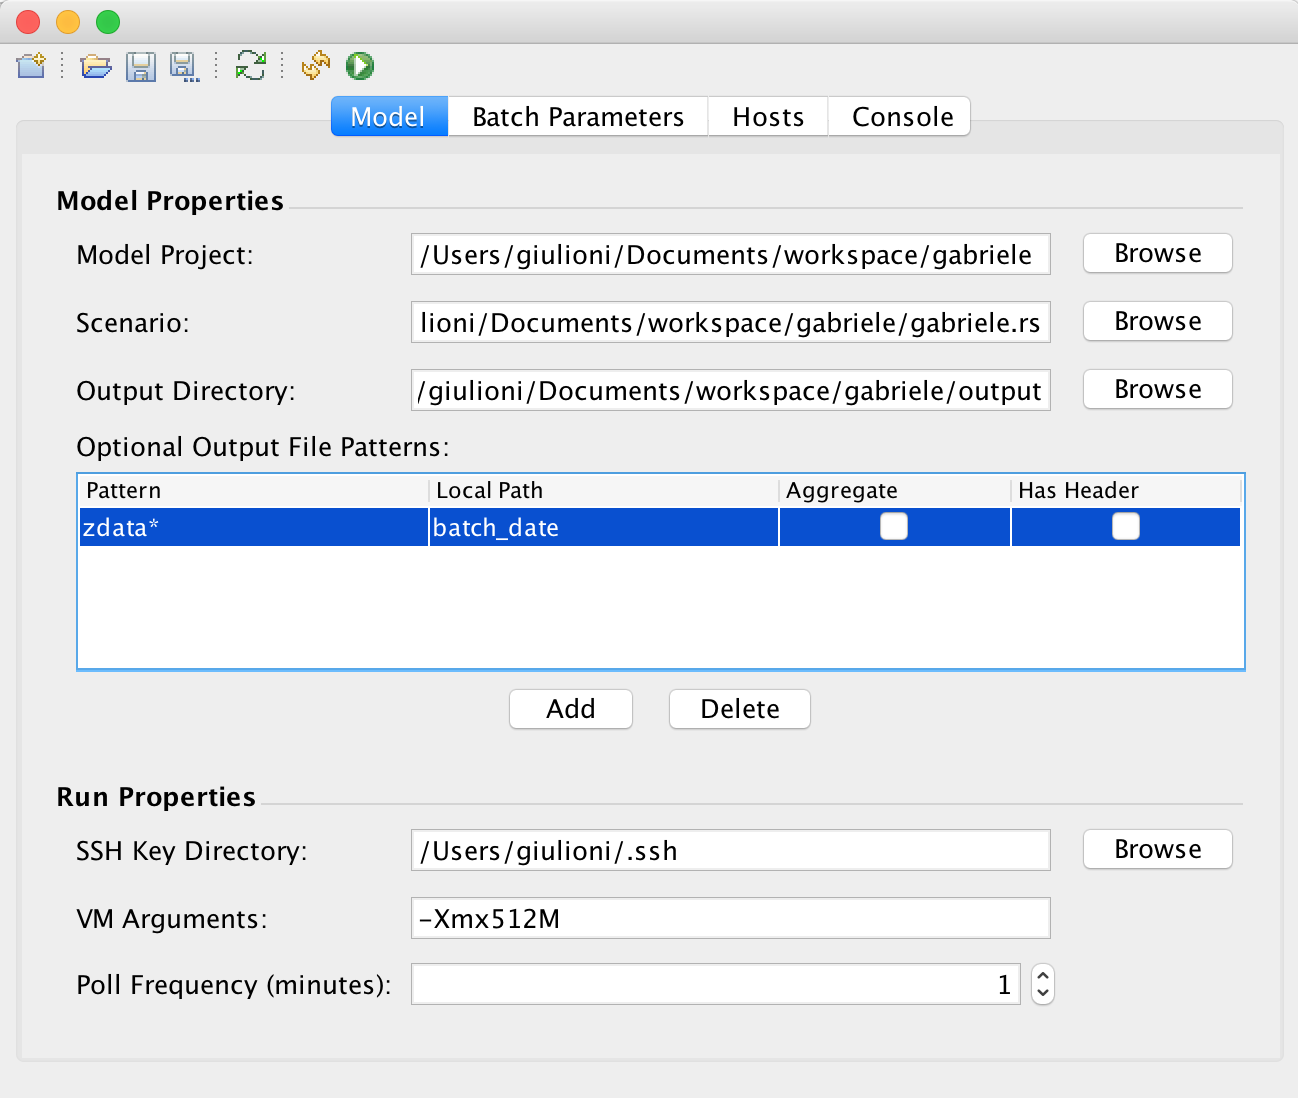
\includegraphics[scale=0.35]{fig_gabriele_rs_batch}

This configuration instructs RS to fetch
all the file whose name begins with \verb+zdata+  
from all the machines running the model in parallel 
and move them in an output sub-folder named 
\verb+batch_date+. Needless to say that the sub-folder name can be chosen at your convenience, and it can be changed at each batch run in order to avoid overwriting the data (perhaps you want to have memory of the time of your runs. It is why we add \verb+_date+ to the folder name).


The following figure shows the contents of the model output folder after a local batch run using Eclipse navigator panel\\ 
\noindent
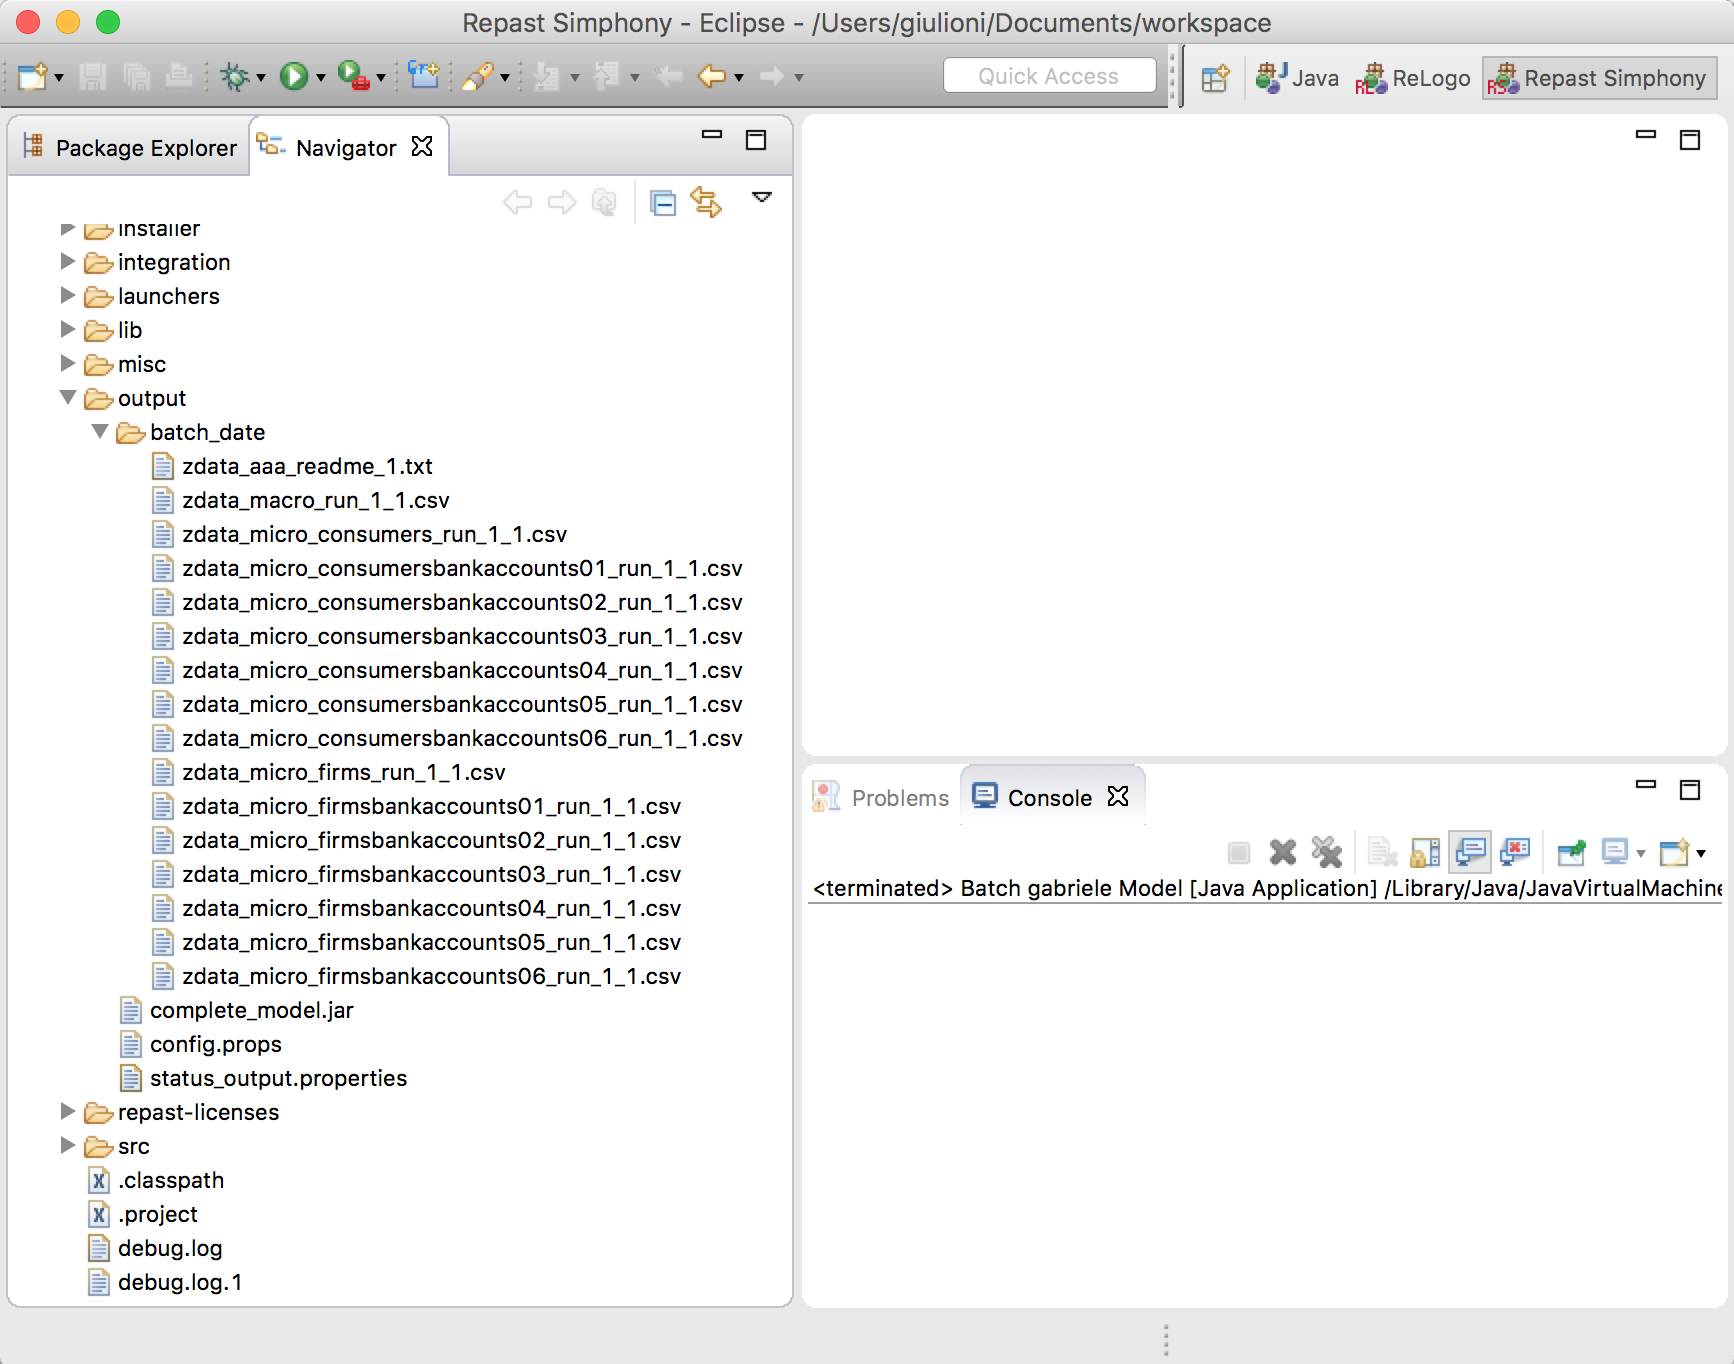
\includegraphics[scale=0.35]{fig_gabriele_rs_batch1}


\chapter{Streamlined Installation}

\section{Installation}
This chapter reports the instructions for installing and running the model in Unix like Operating Systems using a command line approach. Therefore, the instructions will be also valid for Linux and recent Mac machines.

The examples and the command line outcomes given below relate to a user named \verb+coolcoder+. You should easily be able to adapt the paths to you own user account. 

The following colors are used:\\
\color{red}red \color{black} to denote a command;\\
\color{blue}blue \color{black} to denote an ordinary file in command line output;\\
\color{green}green \color{black} to denote an executable file in command line output;\\
\color{magenta}magenta \color{black} to denote the contents of text files.\\

\subsection{Java Development Kit (JDK)}
Follow the instructions given in the previous chapter to install or update JDK if needed. 
\subsection{Repast Simphony (RS)}
Also in this case, you can follow the instructions given in the previous chapter. However, the process therein described implies the installation of eclipse. We will give here an alternative way to install the RS library and to use it directly.

First of all you have to download all the RS library packages.\footnote{Note that the installation process described in RS web site implies downloading the RS library and put them in the eclipse plugins folder.}

You can download all the jars by using the \verb+wget+ command with the recursion option (\verb+-r+).\footnote{If the command is not available in your system you have to install it.}

The following steps have to be taken to install RS.

Suppose, for example, you have the directory \verb+/Users/coolcoder/abm_java_libraries+. Create the directory\\
\verb+mkdir repast+\\
and move into it\\
\verb+cd repast+\\

Download the files from the RS repository\\
%\verb+wget -r http://mirror.anl.gov/repastsimphony/plugins/+\\
\verb+wget -r -l1 --no-parent -nd --no-check-certificate +\\
\verb+             https://repo.anl-external.org/repos/repast/plugins/+\\

Some minutes are needed to complete the download.% Press \verb/ctrl+c/ to release the cursor.

The directory now should contain many jar files.

Give the following command:\\
\verb+ls *.jar|awk -F'.jar' '{print "unzip "$0" -d "$1}'|sh+

Each jar file now has the corresponding folder.
Remove all the jar files by typing:\\
\verb+rm *.jar+

Now the RS library is installed in your system and is ready to be used.
To test your installation type the command:\\
\begin{verbatim}
java -cp /Users/coolcoder/abm_java_libraries/
               repast/repast.simphony.runtime_<version>/lib/*:
         /Users/coolcoder/abm_java_libraries/
               repast/repast.simphony.runtime_<version>/bin 
         repast.simphony.runtime.RepastMain
\end{verbatim}
where you have to replace \verb+<version>+ with the version identification number (for example \verb+2.3.0+).

After a while, the RS GUI window should pop up.

%Close the window because we will run the model in BATCH mode only.



\subsection{GABRIELE}

Now you have to choose or create the GABRIELE destination folder.
Suppose it is called \verb+models+ and has the following absolute path: \\
\verb+/Users/coolcoder/models+

You can use again the two methods described in the previous chapter (git or compressed archive) to install the model. 

Briefly, using git, change directory in \verb+models+ and give the following command:

\vskip2mm
\noindent\verb+~/models$ +\color{red}\verb+git clone https://github.com/ggiulion/gabriele.git+ \color{black}

\vskip2mm
That's it!

Otherwise, you have to download the zip archive: point your browser to\\ 
\verb+https://github.com/ggiulion/gabriele+\\
Click on the ``clone or download'' button and choose ``download zip''.

This will download the \verb+gabriele-master.zip+ file in your system.

Move the archive in\\
\verb+/Users/coolcoder/models+

Unpacking it, the \verb+gabriele-master+ folder is created.

Rename the \verb+gabriele-master+ in \verb+gabriele+.

Delete the \verb+gabriele-master.zip+ file.

\vskip1cm
Regardless of the method used, you should have the following directories tree: 

\begin{verbatim}
/Users/coolcoder/models/gabriele
/Users/coolcoder/models/gabriele/src
/Users/coolcoder/models/gabriele/docs
/Users/coolcoder/models/gabriele/gabriele.rs
/Users/coolcoder/models/gabriele/scenario
\end{verbatim}

Now, \verb+cd+ into the \verb+gabriele+ directory and get its absolute path  



\vskip2mm
\noindent\verb+~/models$ +\color{red}\verb+cd gabriele+ \color{black}\\
\verb+~/models/gabriele$ +\color{red}\verb+pwd+ \color{blue}\\
\verb+/Users/coolcoder/models/gabriele+
\color{black}
\vskip2mm


Save this information because it will be used in the configuration phase. \\ We will refer to it as the model base directory.

\section{Testing the installation}

\subsection{Configuration}

Create a new directory outside the model base directory. \\ We will refer to it as the data directory.

Suppose the data directory is called \verb+gabriele_data+ and has the following absolute path: \\
\verb+/Users/coolcoder/Documents/gabriele_data+

\verb+cd+ into the data directory.

Find out the Repast installation directory:

\vskip2mm
\noindent\verb+~/Documents/gabriele_data$ +\color{red}\verb+sudo find / -name "repast.simphony.core*"+ \color{black}
\verb+Password:+ \\ \color{blue}
\verb+/Users/coolcoder/abm_java_libraries/repast/repast.simphony.core_2.3.1 +\\
\color{black}
\vskip2mm

In this expression, \verb+/Users/coolcoder/abm_java_libraries/repast+ is repast base directory and \verb+2.3.1+ is repast version.

Prepare a text file named \verb+paths.txt+ having the repast base directory in its first line, repast version in the second line and the model base directory in the third line. The file content should look as follows:

\color{magenta}
\vskip2mm \noindent
\verb+/Users/coolcoder/abm_java_libraries/repast+ \\
\verb+2.3.1+ \\
\verb+/Users/coolcoder/models/modelJasss+
\vskip2mm

\color{black}
You must adapt the paths and the repast version of this file to your settings.

Save this file into the data directory.

Move the \verb+configure+ file from the gabriele scenario folder to the data directory:

\verb+mv /Users/coolcoder/models/gabriele/scenario/configure . +


The contents of your data folder is now:

\vskip2mm
\noindent\verb+~/Documents/gabriele_data$ +\color{red}\verb+ls+ \color{blue}\\
\verb+configure+ \\
\verb+paths.txt+
\color{black}

\vskip2mm
Make the \verb+configure+ file executable and run it:

\vskip2mm
\noindent\verb+~/Documents/gabriele_data$ +\color{red}\verb|chmod +x configure| \color{black}\\
\verb+~/Documents/gabriele_data$ +\color{red}\verb|./configure| \color{black}

\vskip2mm
This creates three additional files:

\vskip2mm
\noindent\verb+~/Documents/gabriele_data$ +\color{red}\verb+ls+ \color{blue}\\
\verb+compile+\\ \color{green}
\verb+configure+\\ \color{blue}
\verb+paths.txt+ \\
\verb+run_batch+ \\
\verb+sourcefilespath+
\color{black}

\vskip2mm
Make the \verb+compile+ and \verb+run_batch+ files executable:

\vskip2mm
\noindent\verb+~/Documents/gabriele_data$ +\color{red}\verb|chmod +x compile| \color{black}\\
\verb+~/Documents/gabriele_data$ +\color{red}\verb|chmod +x run_batch| \color{black}
\vskip2mm


\subsection{Running GABRIELE}

We recall that the streamlined installation was built to run the model in BATCH mode in a fast way avoiding the slowness of the batch wizard. Therefore we will only give instruction for the command line batch run.

First of all compile the model by typing:
\vskip2mm
\noindent\verb+~/Documents/gabriele_data$ +\color{red}\verb|./compile| \color{black}
\vskip2mm

The batch run is started with the following command:
\vskip2mm
\noindent\verb+~/Documents/gabriele_data$ +\color{red}\verb|./run_batch| \color{black}
\vskip2mm

When the run completes, you will find the files containing the output of your simulation inside the data directory.
The data file have the \verb+zdata_+ prefix for ease of their identification: 

\vskip2mm
\noindent\verb+~/Documents/gabriele_data$ +\color{red}\verb|ls| \\ \color{green}
\verb+compile+ \\
\verb+configure+ \\ \color{blue}
\verb+paths.txt+ \\ \color{green}
\verb+run_batch+ \\ \color{blue}
\verb+sourcefilespath+ \\
\verb+zdata_aaa_readme.txt+ \\
\verb+zdata_macro_run_1.csv+ \\
\verb+zdata_micro_consumers_run_1.csv+ \\
\verb+zdata_micro_consumersbankaccounts01_run_1.csv+ \\
\verb+zdata_micro_consumersbankaccounts02_run_1.csv+ \\
\verb+zdata_micro_consumersbankaccounts03_run_1.csv+ \\
\verb+zdata_micro_consumersbankaccounts04_run_1.csv+ \\
\verb+zdata_micro_consumersbankaccounts05_run_1.csv+ \\
\verb+zdata_micro_consumersbankaccounts06_run_1.csv+ \\
\verb+zdata_micro_firms_run_1.csv+ \\
\verb+zdata_micro_firmsbankaccounts01_run_1.csv+ \\
\verb+zdata_micro_firmsbankaccounts02_run_1.csv+ \\
\verb+zdata_micro_firmsbankaccounts03_run_1.csv+ \\
\verb+zdata_micro_firmsbankaccounts04_run_1.csv+ \\
\verb+zdata_micro_firmsbankaccounts05_run_1.csv+ \\
\verb+zdata_micro_firmsbankaccounts06_run_1.csv+ \\
\vskip2mm
\color{black}


\part{Understanding GABRIELE}

%\chapter{Introduction}
This model aims at reproducing the dynamics of an economic systems.

The functioning of a dynamic system is described by giving information on the following elements:
\begin{itemize}
	\item the components of the systems, 
	\item how they behave and 
	\item how they interact with each other. 
\end{itemize}

%Throughout this document we will extensively use the two visual representations reported in figures \ref{fig:components} and \ref{fig:sequence}. 

Chapter \ref{chap:components} aims at showing the \textbf{model components}.


Chapter \ref{chap:events} describes the dynamics of events. This includes the initialization phase which is performed just once at the beginning of the simulation and the \textbf{sequence of events} repeated in each time step.


%In the following subsections we will carefully describe these two representations because they will be used in combination throughout the whole document. 



\newpage

%\subsection{System Components}
\chapter{The components of the system}\label{chap:components}

Figure \ref{fig:components} gives a visual representation of the system components.

\begin{figure}[htp]
\hskip-1cm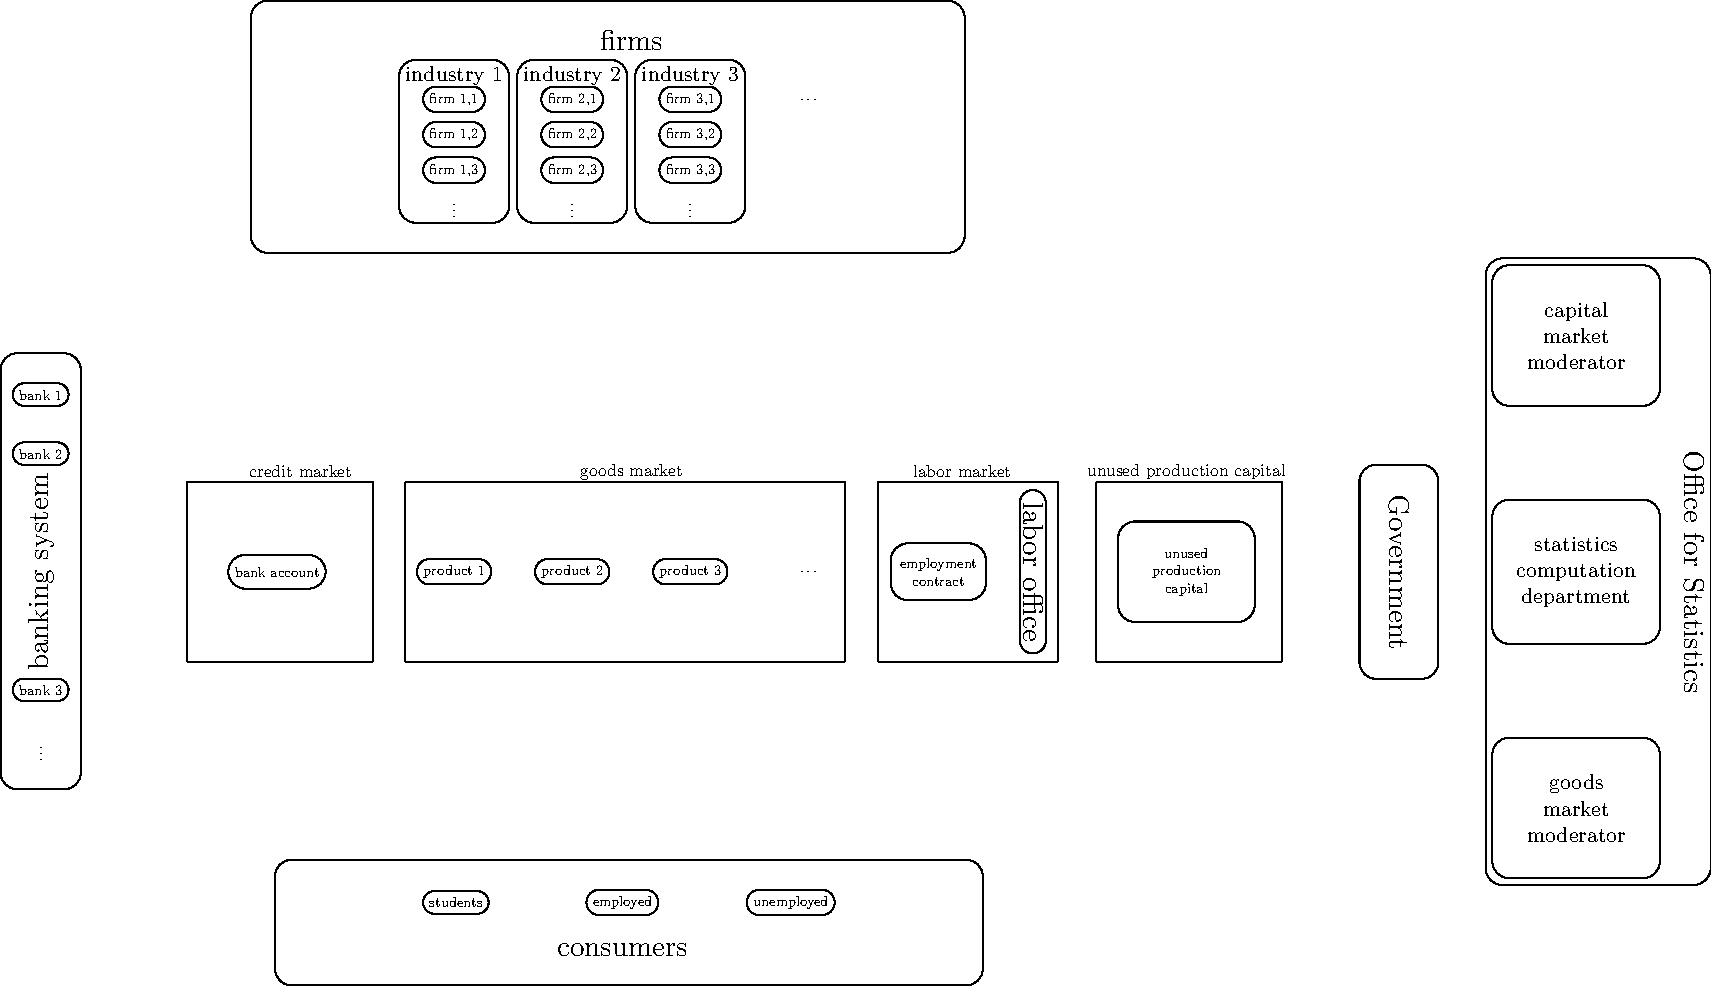
\includegraphics[scale=0.5]{agents_and_interactions_figure1-0.pdf}
	\caption{Components of the economic system}
	\label{fig:components}
\end{figure}
For a systematic description of the system components, we divide them in the following categories:
\begin{itemize}
	\item agents;
	\item goods;
	\item financial assets.
\end{itemize}
\section{Agents}
%The standard economic modeling characterization is used. The model is therefore populated by the following agents:

Let us distinguish between multi-instances and single-instance agents.  

In this version of the model, Multi-instances agents are
\begin{itemize}
	\item consumers
	\item firms
	\item banks
\end{itemize}
while single-instance agents are:
\begin{itemize}
	\item government
	\item labor office
	\item Office for statistics
\end{itemize}

Multi-instances agents are grouped in sectors: the consumers, firms and banking sectors. Adding the government to these three sectors, we obtain the usual categorization of the economy into the four institutional sectors: households, firms, financial sector and public sector. Figure \ref{fig:componentsc1} highlights the institutional sectors in light blue.
\begin{figure}[htp]
\hskip-1cm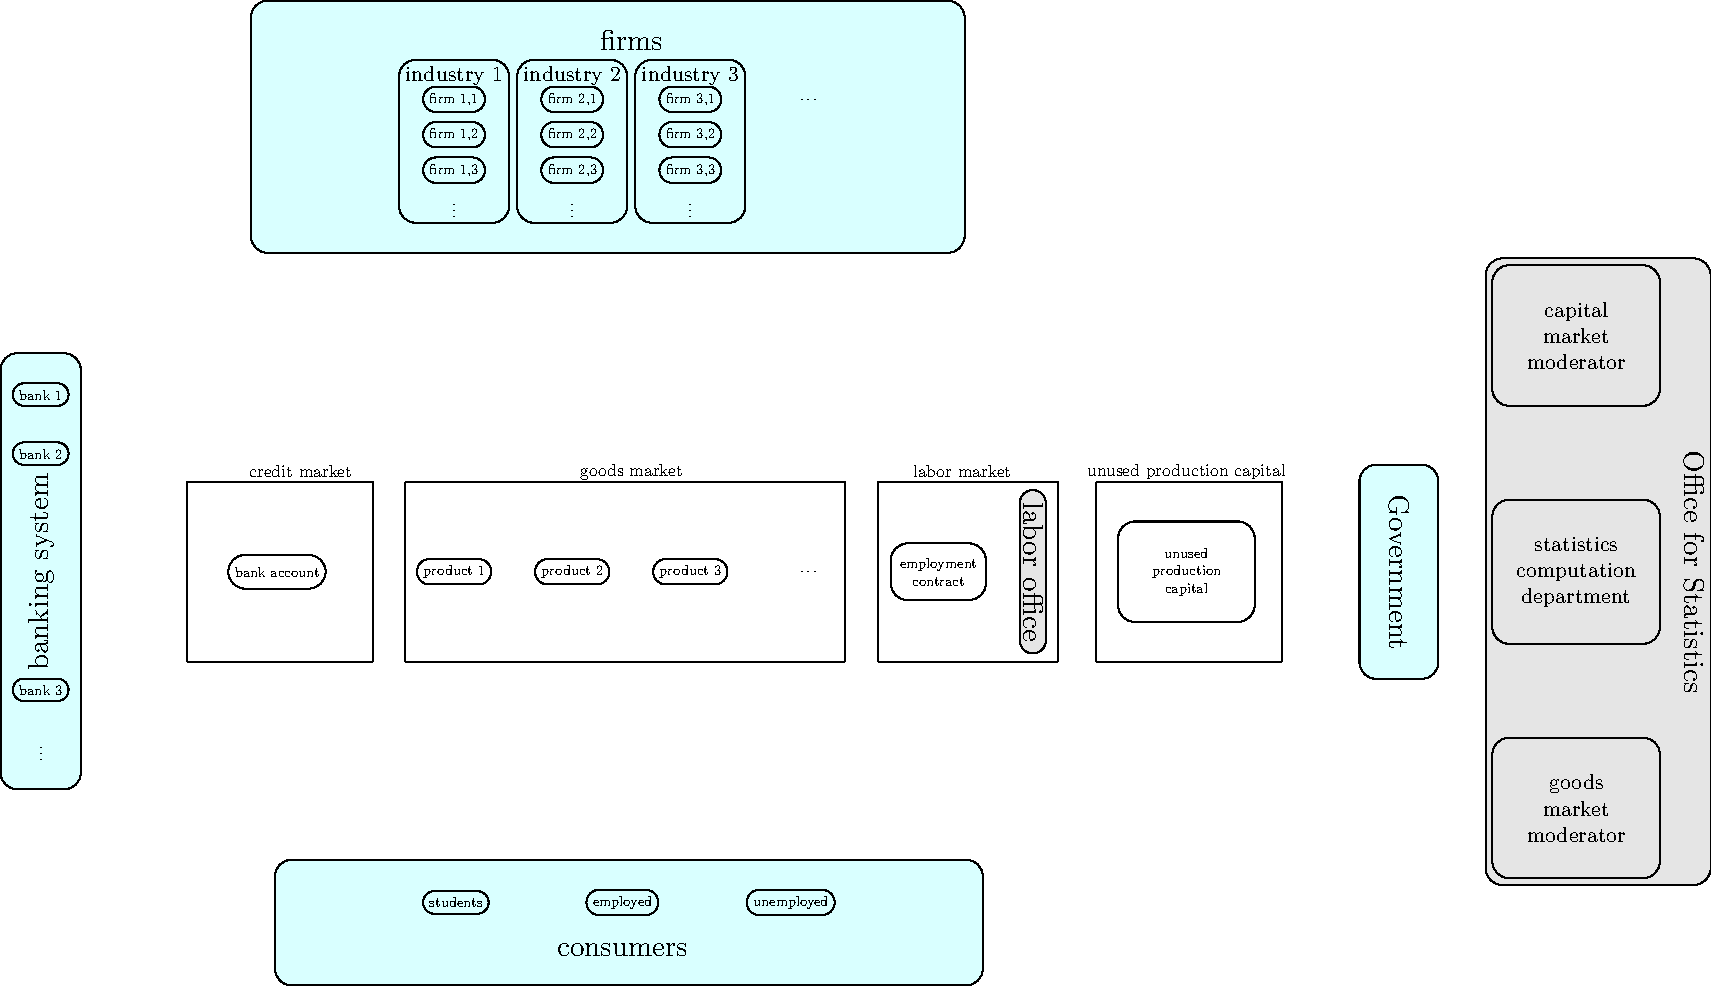
\includegraphics[scale=0.5]{agents_and_interactions_figure1c1-0.pdf}
	\caption{Components of the economic system: institutional sectors and other single-instance agents.}
	\label{fig:componentsc1}
\end{figure}
The other two single-instance agents are highlighted in gray: the Labor Office operates in the labor market, while the Office for Statistics, has a global view of the system. The latter computes aggregate variables making them available to all the other agents. Furthermore, it uses this information to moderate the goods and production capital markets.

Figure \ref{fig:componentsc1} also shows the internal structure of the firms and consumers sectors. 

Consumers are classified in students and non-students. The latter in turn can be employed and unemployed. Therefore, each consumer of the model falls into one of the these three groups: student, worker and unemployed.

The internal structure of the firms sector is designed to allow for product differentiation. In case the researcher is interested in having multiple products, firms are organized into industries that groups firms making similar item.


\clearpage
\section{Goods}
In this section we focus on the real part of the model while the financial part is treated in the next section.

In the present version of the model, the real part of the economy consists in exchanges of the following items:
\begin{itemize}
	\item consumption goods
	\item production inputs
		\begin{itemize}
			\item investment goods
			\item labor
		\end{itemize}
\end{itemize}

These items are exchanged in the three corresponding markets highlighted in gray in figure \ref{fig:componentsc2}.


\begin{figure}[htp]
\hskip-1cm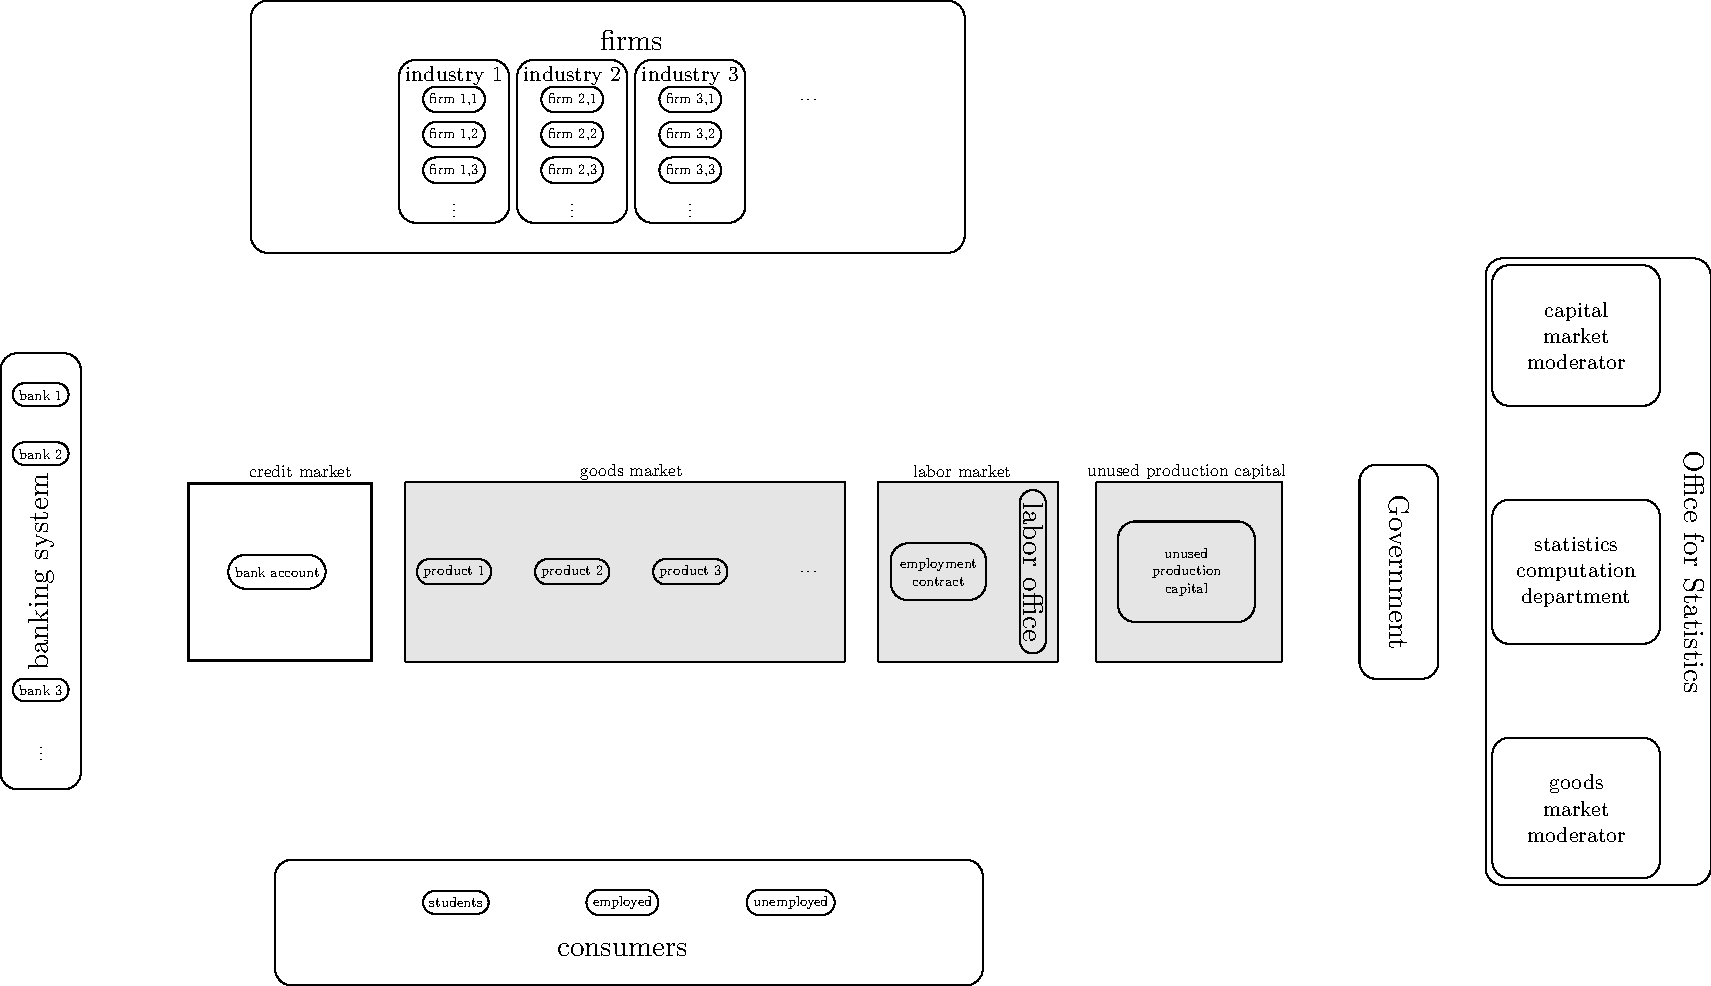
\includegraphics[scale=0.5]{agents_and_interactions_figure1c2-0.pdf}
	\caption{Components of the economic system: real markets.}
	\label{fig:componentsc2}
\end{figure}

As explained above, the model allows for product differentiation. It concerns consumption products. We have signaled this possibility by indexing the products in the goods market.

Firms production capacity can be increased in two ways: by buying existing unused production capital or by buying newly produced investment goods. 
To avoid the complication of including a specific industry producing investment goods, the following device is used. Investment goods are realized by assembling the existing consumption goods. Therefore, demand for new investment goods increases the demand in the consumption goods markets. Once assembled, these goods becomes production capital, and are accounted as assets in the firms balance sheet. Production capital used in the production process gradually depreciates. It can happen that a firm has an excess of production capital (especially in case of a decreasing demand). In this case, the firm can decide to offer the unused production capital on the corresponding market. 
Firms having shortages of production capital, first check for its availability on the market for unused production capital. If, after these exchanges, additional production capital is needed, the firm asks for new product in the consumption goods market. The latter are then assembled to obtain new production capital. On the other hand, it can happen that the amount of existing unused production capital is larger than the amount asked on the market. In this case, the exceeding production capital that cannot be sold gradually depreciates at a depreciation rate that can be set at a different level to that wearing away the production capital employed in the production.

Finally, to realize the production, labor is needed.  The labor market completes the set of real markets of this model.  

More details on the markets functioning are given in the next part of the manual.

\clearpage
\section{Financial assets}

In the previous section we have identified the type of goods in our model. The identification and specification of financial products to be included in the model are equally important and are performed in this section. 

In the present version of the model, we include the financial contract which is the cornerstone of nowadays financial systems: the bank account.

In this model, every consumer or firm has at leas one bank account. The bank account is a convenient modeling device: it can be either used to store wealth or as a means to obtain credit. In the latter case, the amount on the bank account will be negative.

Having no other financial contracts, in the present version of the model we have intermediated finance only. %Some agents have positive bank accounts (deposits) while others have negative bank accounts borrowing from the bank. 
Financial exchanges are thus performed in the credit market (highlighted in gray in figure \ref{fig:componentsc3})

\begin{figure}[htp]
\hskip-1cm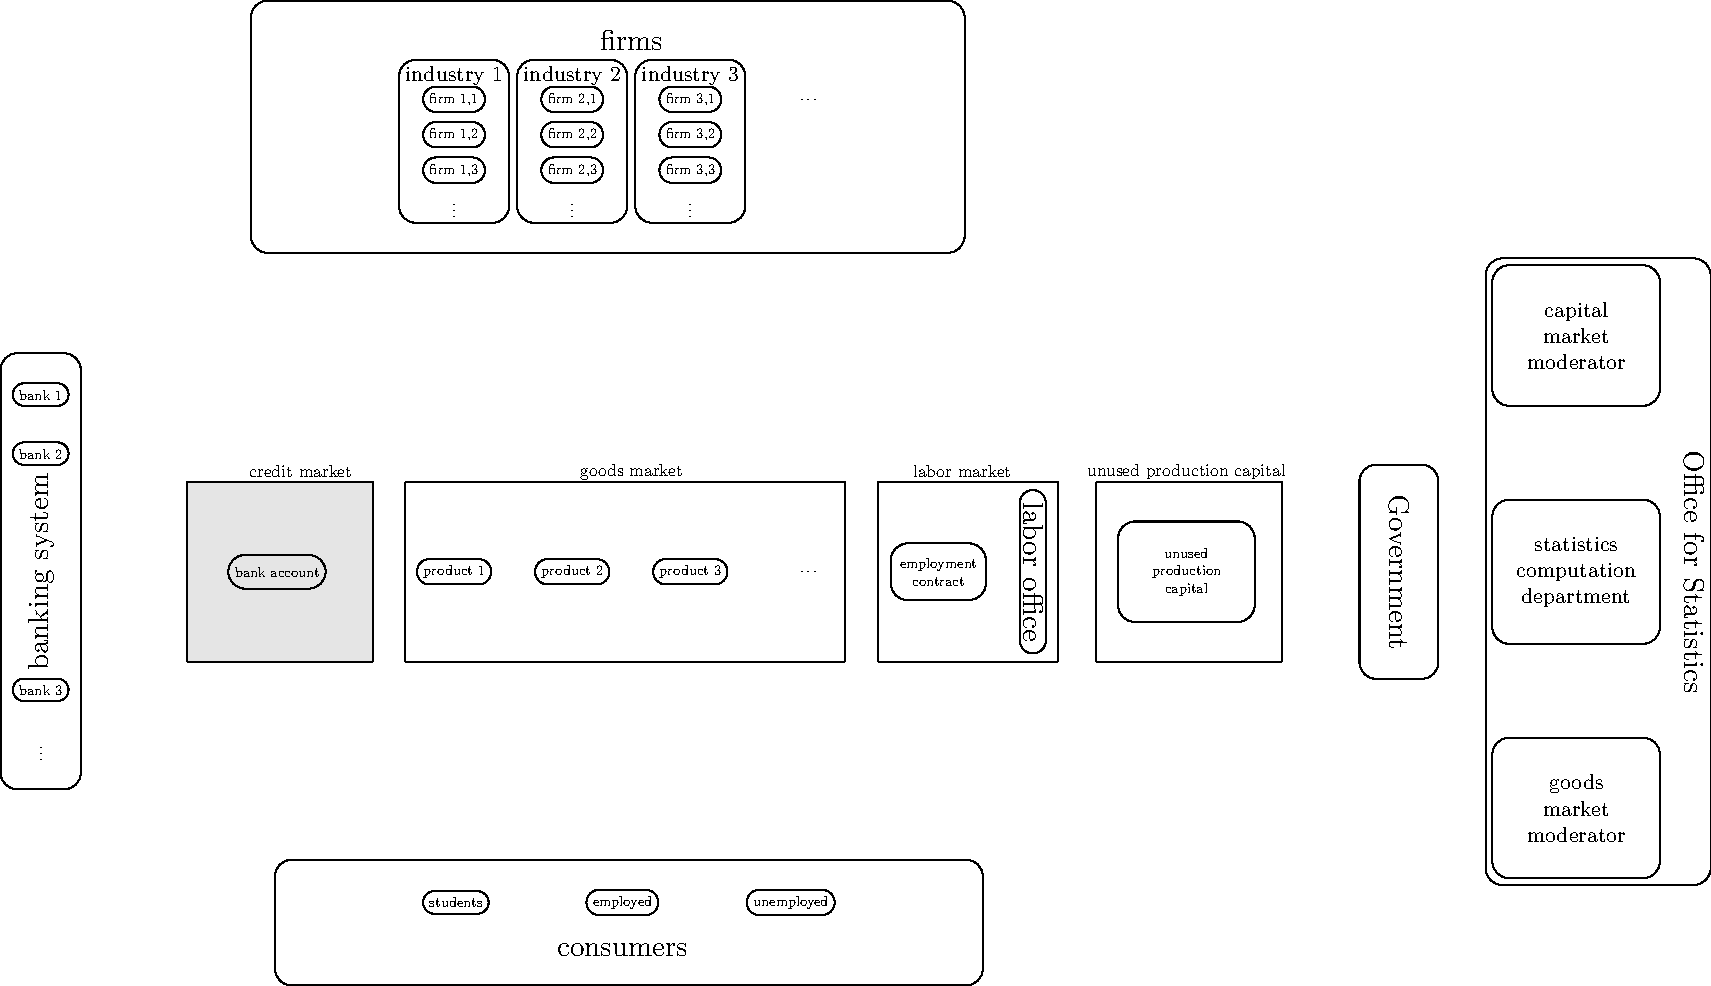
\includegraphics[scale=0.5]{agents_and_interactions_figure1c3-0.pdf}
	\caption{Components of the economic system: the credit market.}
	\label{fig:componentsc3}
\end{figure}

Considering additional financial contracts, and therefore adding other financial markets to the model, is a goal for the near future. This enrichment will allow the model gradually approach the reality of nowadays financial markets.




\newpage
\chapter{The Dynamics of Events}\label{chap:events}

We start the description by the visual representation of the dynamics of events given in figure \ref{fig:sequence}. The figure shows that after the initialization phase (that will be detailed in section \ref{sec:initialization}) the software enters in the main loop (deeply discussed in section \ref{sec:mainloop}). Figure \ref{fig:sequence} gives a brief description of the various events together with the information on the agent(s) involved in them. To save space we use the following abbreviations:

\begin{itemize}
	\item $OFS$: office for statistics
	\item $G$: Government
	\item $CB$: Central Bank
	\item $F$: firms
	\item $C$: consumers
	\item $C_S$: the subset of consumers that are students
	\item $C_E$: the subset of consumer that are employed
	\item $C_U$: the subset of consumer that are unemployed
	\item $B$: banks
	\item $LM$: labor market
\end{itemize}

When an event implies a flux from an agent to another, an arrow is added to give this information. As an example,\\
$C \rightarrow B$: pay back if possible\\
stands for: Consumers refund banks if possible.

The initialization and the main loop are detailed in the following subsections.

\begin{figure}[htp]
	\centering
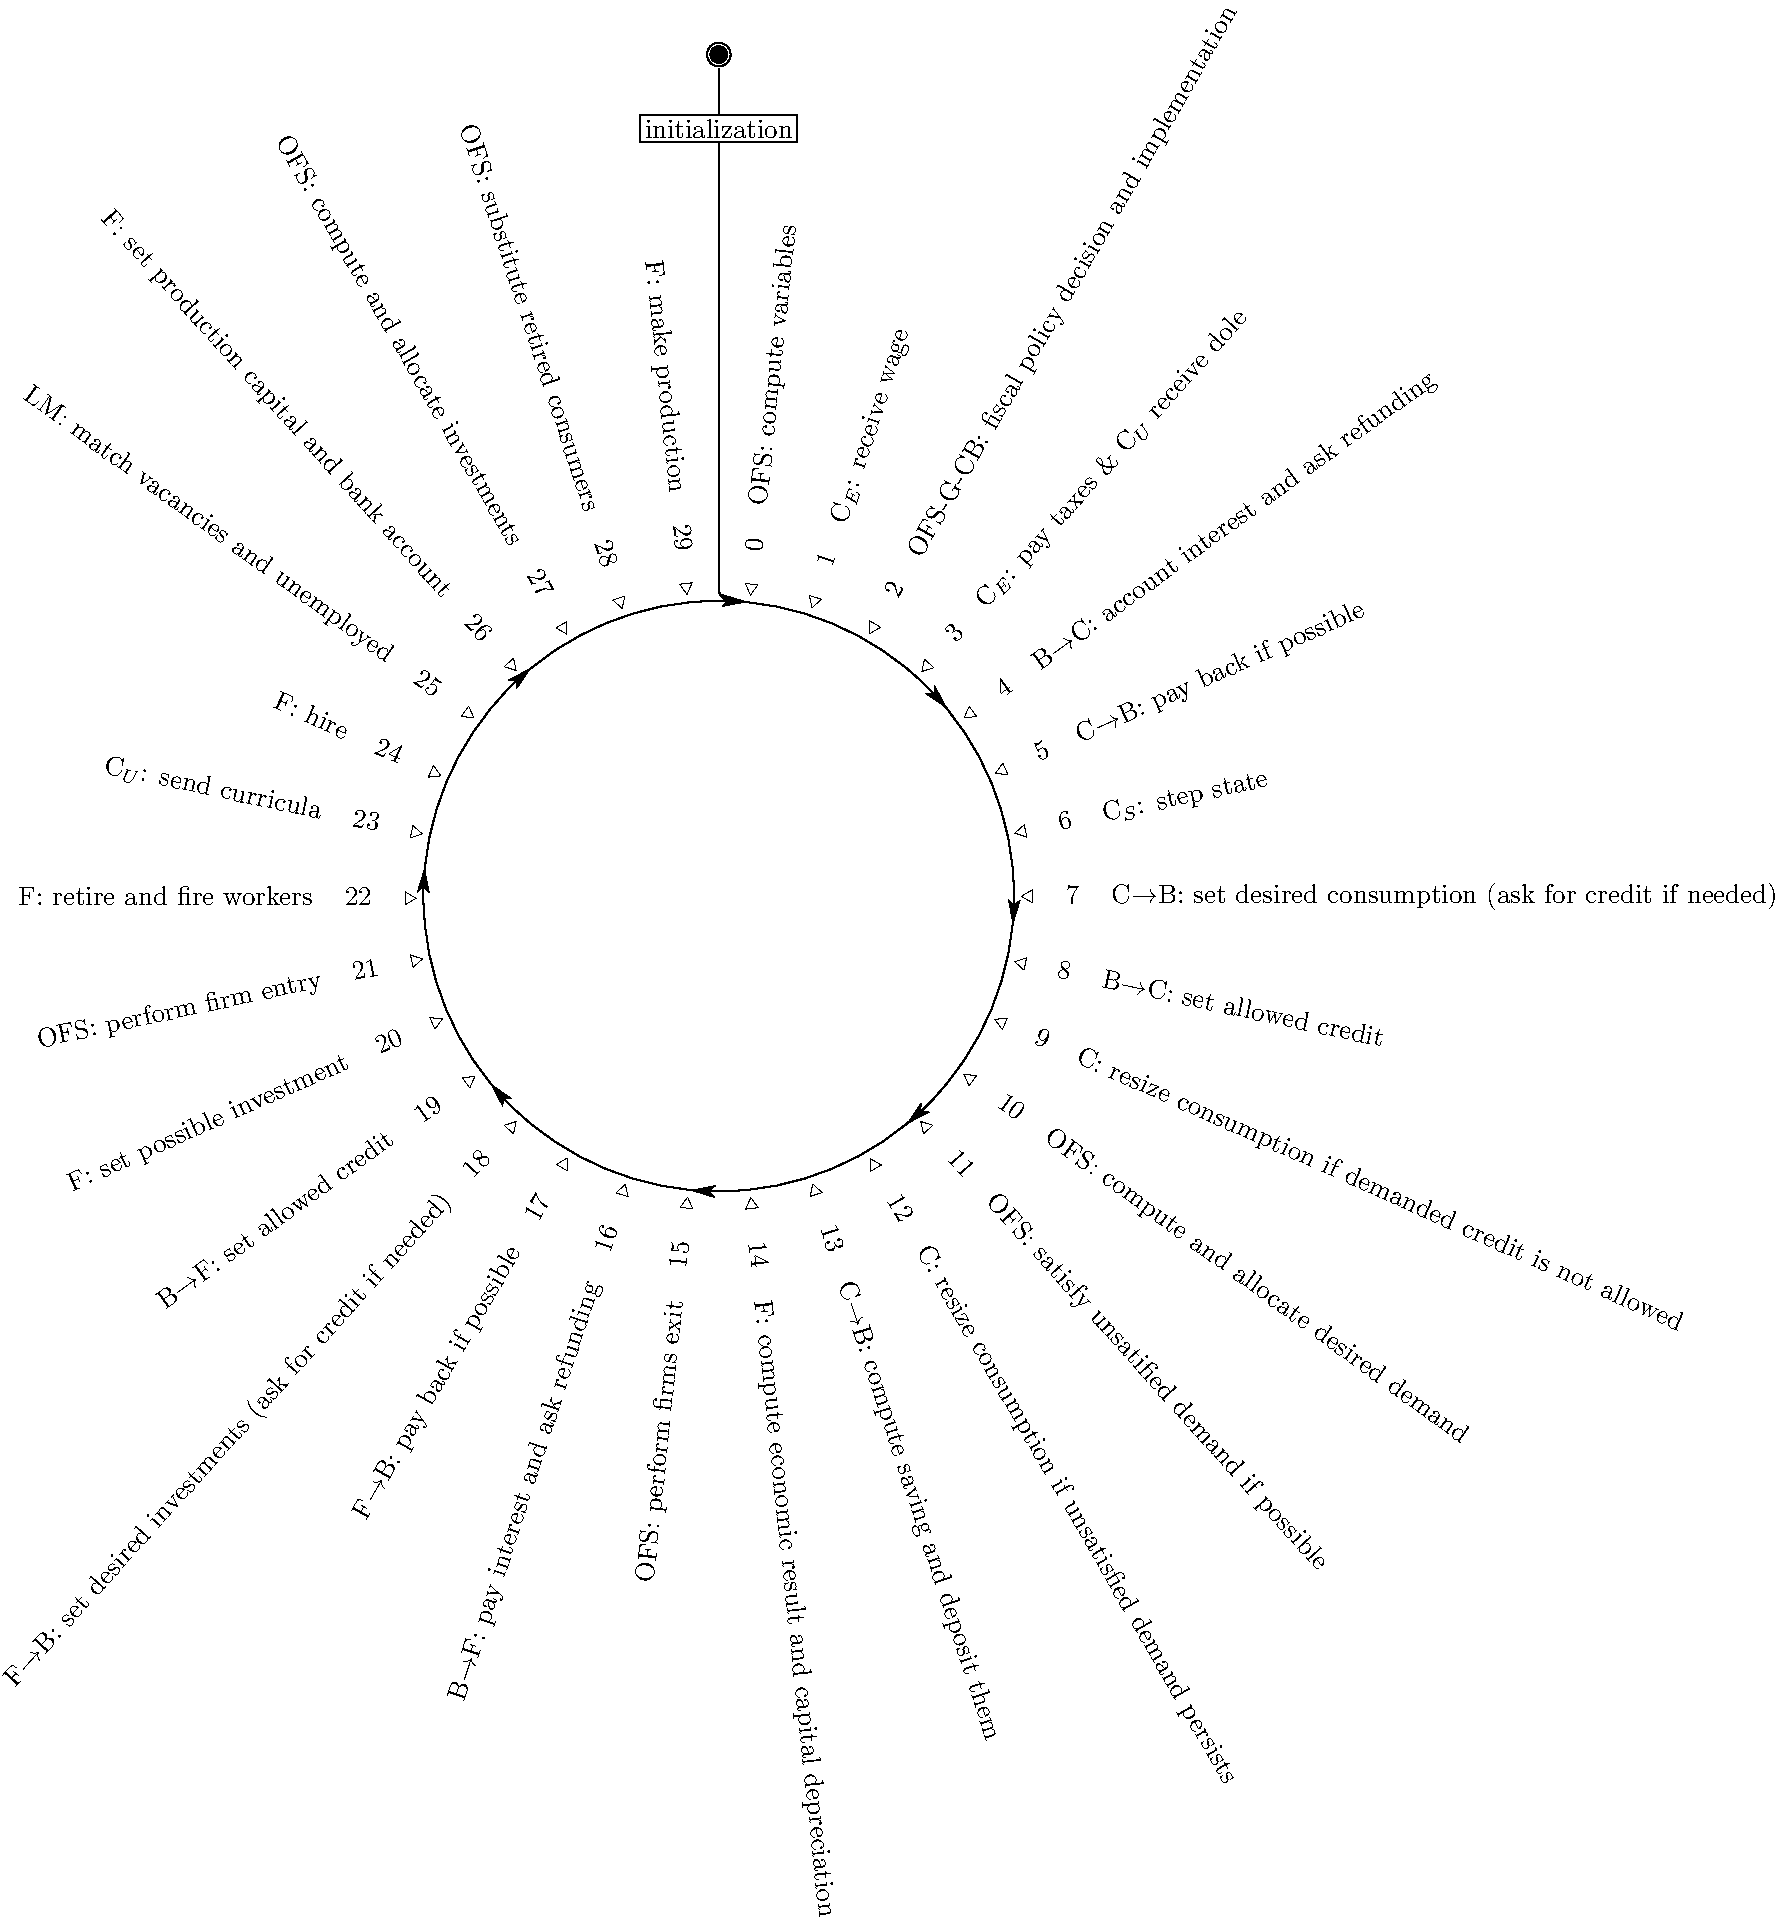
\includegraphics[scale=0.5]{visual.pdf}
	\caption{sequence of events}
	\label{fig:sequence}
\end{figure}

\clearpage
\section{Initialization}\label{sec:initialization}
The initialization phase aims at setting firms' potential production.  %  to determine their initial production. reducing exogenous setting to the minimum. 
After this step,  
%When the initial level of production is computed,  
the sequence of events can progress by entering the main loop. During the initialization process, the stock variables of all agents are set in a consistent way.\begin{marginfigure}
	\hskip1cm
\includegraphics[scale=1.0]{sc_logo-0.pdf}
\end{marginfigure}


The details on the initialization process are given hereafter.

\label{pg:inputs1}
To realize production firms need two production input: capital and labor. We use the following Leontief type production function:
\begin{equation}
Y_f=\min(Y_f^{PK},Y_f^{PL})
	\label{eq:production_function}
\end{equation}
According to this function, production realized by firm $f$, \gls{var:Yf}, is the minimum between the potential production that can be realized with the outstanding production capital without labor constraints, \gls{var:YPKf}, and the potential production that can be obtained by the labor force employed by the firm without capital constraint, \gls{var:YPLf}. 


The capital potential production is assumed to be equal to the level of capital (\gls{var:Kf}):
\[
	Y^{PK}_f=K_f
\]

Computing the potential production of labor is more tricky because workers are heterogeneous and have different productivities. 
We will explain in details how workers' productivities are set in the next section when the consumers initialization will be discussed. For now, it is enough to know that labor is heterogeneous and that a worker's productivity will be identified with \gls{var:psiwf}.  To compute the potential production of the workforce employed in a firm, the sum of workers productivities is first computed:
\[
	\psi_f=\sum_{w \ \textnormal{ working in} \ f}\psi_{w,f}
\]
Then, we introduce the following\\ 
parameter:\\
\begin{tabular}{l l l l}
	\hline
	& &&read\\
	notation& name &&from\\
	in equations& in code&value&file\\
	\hline
	\hline
	\gls{par:thetaYL}&\verb+parameterOfProductivityInProductionFuncion+&100&yes\\
	\hline
\end{tabular}

\vskip5mm

The potential production of labor is finally computed as:
\[
	Y^{PL}_f=\theta_{YL}\psi_f.
\]




To arrive at the very first $Y_f$,  several preliminary steps, such as initializing the working state of each consumer, are needed. Some of these steps call for additional operations such as setting up the various agents balance sheets and checking for their consistency.
In the remainder of this section we sketch the process, while more details will be given in the following sections.

We adopt the following strategy to set $Y^{PL}_f$ and $Y^{PK}_f$: 
\begin{itemize}
	\item compute the potential output from workers
	\item adjust capital such as the potential output from capital is equal to the potential output from workers 
\end{itemize}

As already mentioned, the first step implies a preliminary setup of household working state. The second step, instead, allows the setup of firms assets balance sheet item. 

Knowing firms balance sheet assets, we set the liabilities in such a way that the balance sheet identity is satisfied.

Next, we initialize the household balance sheet.

Once the amount of households' and firms banks accounts are known, we setup banks balance sheets.

So the whole initialization sequence has the following phases:
\begin{enumerate}
	\item create agents;
	\item set consumers working state;
	\item compute each firm labor potential production and set the production capital to a level that allows a potential production equal to that of labor;
	\item set agents balance sheet;
	\item revise agents balance sheet for stock consistency.\begin{marginfigure}
	\hskip1cm
\includegraphics[scale=1.0]{sc_logo-0.pdf}
\end{marginfigure}

\end{enumerate}

These phases are explained in details in the \href{\doclocation/index_initialization.html}{technical documentation}. There, we present the steps taken for initializing the model in a sequential order. We also document the above mentioned phases by using UML activity diagrams.

Readers that would not delve into the technical documentation at this point can progress to the following sections where we discuss deeply the initialization for each type of agent.

\subsection{Consumers initialization}

\subsubsection{Working situation}


\subsubsection*{Students}
\label{pref:tudentevolution}

Each worker is characterized by its fundamental ability. It characterizes each consumer performance during the education period. The latter in turn determine the productivity as a worker.

We call this parameter the ability (as) student and denote it \gls{par:thetaas}. We set it during initialization by drawing from a uniform distribution \gls{par:Thetaas}:
\[
	\Theta_{as}\sim U(\theta_{minas},\theta_{maxas})
\]
The following parameters are thus used:\\
\begin{tabular}{l l l l}
	\hline
	& &&read\\
	notation& name &&from\\
	in equations& in code&value&file\\
	\hline
	\hline
	\gls{par:thetaminas}&\verb+Context.minAbilityStudent+&$0.35$&yes\\
 \gls{par:thetamaxas}&\verb+Context.maxAbilityStudent+&$0.5$&yes\\
	\hline
\end{tabular}

\vskip5mm
The most important observation about this parameter is that its upper value is 0.5.

Another important variable is the consumers age, which is initialized as a random number between zero and the parameter \gls{par:thetacea} denoting the retirement age:\\

\vskip2mm
\noindent
\begin{tabular}{l l l l}
	\hline
	& &&read\\
	notation& name &&from\\
	in equations& in code&value&file\\
	\hline
	\hline
\gls{par:thetacea}&\verb+Context.consumerExitAge+&$70$&yes\\
	\hline
\end{tabular}

\vskip5mm
Using the \verb+abilityStudent+ and the \verb+consumerAge+ the education history of consumers is initialized. Each year of education is set to successful if that year uniform random draw $u$ is less that two times the student ability:\footnote{Note how $2\theta_{c,as}\le 1$ and $u$ is drawn from a $U(0,1)$.}
\[
	u<2\theta_{c,as}
\]
and unsuccessful otherwise.  Note that best students has $\theta_{c,as}=0.5$, so they will be alway successful because $2\theta_{c,as}=1$. Students with less abilities has lower probability to be successful.\\

To initialize the education history we use the following\\ 
parameters:\\

\noindent
\begin{tabular}{l l l l}
	\hline
	& &&read\\
	notation& name &&from\\
	in equations& in code&value&file\\
	\hline
	\hline
\gls{par:thetamnfpe}&\verb+maxNumberOfFailedPeriodsOfEducation+&$2$&yes\\
\gls{par:thetamnpe}&\verb+maxNumberPeriodsOfEducation+&$21$&no\\
	\hline
\end{tabular}

\vskip5mm


Starting from age 0, the process is repeated until 
\begin{enumerate}
	\item the maximum number of failures admitted ($\theta_{mnfpe}$) or
	\item the maximum periods of possible education ($\theta_{mnpe}+\theta_{mnfpe}$) or
	\item the consumer's age 
\end{enumerate}
is reached.

We then count the number of successful periods of education, \gls{var:nsye}. 

When the process is stopped by conditions 1 or 2, the consumer state is set to non students. At this stage, all non students are unemployed. This state will be revised in the next step. Both the education degree and the productivity as a worker are assigned using \gls{var:nsye}. 

The degree of education is assigned as follows:
\[
	\begin{tabular}{l l l}
	\hline
	$n_{c,sye}$& \textnormal{degree}& \textnormal{degree id}\\
	\hline
	$0\le n_{c,sye}<5$ & \textnormal{none}&0\\
	$5\le n_{c,sye}<8$ & \textnormal{elementary}&1\\
	$8\le n_{c,sye}<13$ & \textnormal{intermediate}&2\\
	$13\le n_{c,sye}<16$ & \textnormal{college}&3\\
	$16\le n_{c,sye}<18$ & \textnormal{bachelor}&4\\
	$18\le n_{c,sye}<21$ & \textnormal{master}&5\\
	$21= n_{c,sye}$ & \textnormal{PhD degree}&6\\
	\hline
	\end{tabular}
\]

The productivity is assigned as follows. Each year of education increases the consumers ability by a fixed amount. So, the productivity (\gls{var:psic}) assigned to a consumer  with \gls{var:nsye} successful year of education is
\[
	\psi_c=\theta_{c,as}+0.5\frac{n_{c,sye}}{\theta_{mnpe}}
\]
Note that \gls{par:thetaas} $=0.5$ implies $n_{c,sye}=$ \gls{par:thetamnpe} so that $\psi_c=1$.

Once the productivity of a non student is known, we compute his/her potential production \gls{var:YPc} as the product of \gls{par:thetaYL} and \gls{var:psic}: 
\[Y^{P}_c=\theta_{YL}\psi_c\]

The education history initialization is stopped by condition 3 when the consumer is young. In this case the subject is assigned the state of student and its education history will be evolved in the main loop using the rules explained above.

\subsubsection*{Employed and unemployed}

At this stage all non students are unemployed. Now, some of them will be employed by firms. 

To perform this task we introduce the following parameter:

\vskip2mm
\noindent
\begin{tabular}{l l l l}
	\hline
	& &&read\\
	notation& name &&from\\
	in equations& in code&value&file\\
	\hline
	\hline
	\gls{par:thetaptbub}&\verb+Context.probabilityToBe+&&\\
	&\hskip2cm\verb+UnemployedAtTheBeginning+&$0.2$&yes\\
	\hline
\end{tabular}

\vskip2mm
With probability $1-\theta_{ptbub}$, each non student selects a firm randomly and send his/her CV to this firm. Subjects who do not send a CV (this happens with probability $\theta_{ptbub}$) enter the main loop in the unemployment state. 

\subsubsection{Initializing consumers bank account}

This is the first action performed to setup the consumers balance sheet. Other actions will contribute to the formation of the consumers' bank account.  

The involved parameters are:\\
\begin{tabular}{l l l l}
	\hline
	& &&read\\
	notation& name &&from\\
	in equations& in code&value&file\\
	\hline
	\hline
 \gls{par:thetanbcc}&\verb+Context.numberOfBanksAConsumerCanBeCustumerOf+&$1$&yes\\
 \gls{par:thetamincba}&\verb+Context.minConsumerInitialBankAccount+&$-500$&yes\\
 \gls{par:thetamaxcba}&\verb+Context.maxConsumerInitialBankAccount+&$500$&yes\\
	\hline
\end{tabular}

\vskip5mm

Each consumer selects randomly a number of banks equal to $\theta_{nbcc}$ and open a bank account in each of them. To set the amount of each bank account the code draw a random integer from a uniform distribution $U(\theta_{mincba},\theta_{maxcba})$. In case the figure is negative the amount is set to zero and the drawn number is assigned to the \verb+demandedCredit+ variable (it will be managed later in the initialization process). Non negative number are assigner to the bank account amount.

As hinted at above, the amount of the various bank accounts will be revised in the final step of the initialization to ensure all the agents' balance sheet consistency.\begin{marginfigure}
	\hskip1cm
\includegraphics[scale=1.0]{sc_logo-0.pdf}
\end{marginfigure}


\subsection{Firms initialization}
\subsubsection{Potential production of labor}
In the consumers initialization we saw that some non student sent their CV to firms.
So, each firm now has a list of CVs. Each firm employs all the senders of the CVs that are in the received CVs list. The CV senders state is switched from unemployed to employed.

As already explained at the beginning of this section, the firm determines the potential production of its labor force (\gls{var:psif}) by summing the potential production of each employee (\gls{var:psiwf}):
\[
	\psi_f=\sum_{w \ \textnormal{working in} \ f}\psi_{w,f}
\]
the potential production is thus
\[
	Y^{PL}_f=\theta_{YL}\psi_f
\]

\subsubsection{Production capital}
As we told above, due to the Leontif production function, the production capital is set in such a way that the potential production from capital is equal to the potential production of labor. We have already defined the potential production of capital as
\[Y_f^{PK}=K_f\]
So, the initial level of capital (\gls{var:Kf}) for each firm is set to
\[
K_f=Y^{PL}_f
\]

\subsubsection{The level of production}

Now that the levels of both production inputs are known, the production made by each firm is computed by using equation (\ref{eq:production_function}).

\subsubsection{Initialization of firms balance sheet}

In the previous step we set up the assets side of the firms balance sheet that is equal to the production capital.

As explained above, we have two liabilities: equity and bank account. We set up equity and determine the bank account residually.

To setup equity we use the following parameters:

\noindent
\begin{tabular}{l l l l}
	\hline
	& &&read\\
	notation& name &&from\\
	in equations& in code&value&file\\
	\hline
	\hline
 \gls{par:thetaminfier}&\verb+Context.minFirmInitialEquityRatio+&$0.1$&yes\\
 \gls{par:thetaminfier}&\verb+Context.maxFirmInitialEquityRatio+&$0.3$&yes\\
	\hline
\end{tabular}

\vskip5mm
Each firm equity base (\gls{var:Ef}) is set as follow
\[
	E_f=u_{Ef}K_f
\]
where $u_{Ef}$ is drawn from $U(\theta_{minfier},\theta_{maxfier})$.

Finally, each firm sets her debt (\gls{var:Bf}) by using the balance sheet identity:
\[
B_f=K_f-E_f
\]

As specified above, debt is obtained through bank accounts.
In this version of the model a firm is costumer of a number of banks given by the following\\
parameter:

\vskip2mm
\noindent
\begin{tabular}{l l l l}
	\hline
	& &&read\\
	notation& name &&from\\
	in equations& in code&value&file\\
	\hline
	\hline
 \gls{par:thetanbfc}&\verb+Context.numberOfBanksAFirmCanBeCustumerOf+&$1$&yes\\
	\hline
\end{tabular}

\vskip2mm
Each firm selects randomly a number of banks equal to \gls{par:thetanbfc} and open a bank account in each of them. The amount of the bank account (\gls{var:BAfb}) is set to
%zero (will be assigned in the next step when the bank balance sheet will be initialized), but the variable demanded credit in each bank account is set to:
\[
	BA_{fb}=-\frac{B_f}{\theta_{nbfc}}
\]

\subsection{Banks initialization}
We remember that in this version of the model, we have only one financial contract: the Bank account ($BA$). Bank accounts can have a positive amount or a negative one. Hereafter, we denote a bank account with a positive amount with \gls{var:BA+} and \gls{var:BA-} denotes a negative amount.

To setup the banks balance sheet, we start again from their assets. Bank assets are households' and firms financial liabilities. In this version of the model, financial liabilities are given by negative bank accounts. 
The sum of negative bank accounts gives the loans extended by a bank (\gls{var:Lb}):
\[
	L_b=\sum_f BA_{fb}^- + \sum_c BA_{cb}^-
\]



Given assets of a bank, we setup the its equity (\gls{var:Eb}) by using the following\\
parameters:\\
\begin{tabular}{l l l l}
	\hline
	& &&read\\
	notation& name &&from\\
	in equations& in code&value&file\\
	\hline
	\hline
 \gls{par:thetaminbier}&\verb+Context.minBankInitialEquityRatio+&$0.1$&yes\\
 \gls{par:thetamaxbier}&\verb+Context.maxBankInitialEquityRatio+&$0.3$&yes\\
	\hline
\end{tabular}

\vskip5mm
A bank equity base is then computed as
\[
	E_b=u_{Eb}L_b
\]
where $u_{Eb}$ is drawn from $U(\theta_{minbieb},\theta_{maxbieb})$.

Now, the level of deposits (\gls{var:Db}) compatible with the balance sheet relationship is computed:
\[
Dep_b=L_b-E_b
\]

Due to the random elements in the initialization of consumers and firms, the normal situation at this stage of the initialization is a stock inconsistency:
\[
	\sum_{c \textnormal{ customer of } b} BA^+_{cb} \neq Dep_b
\]
Note that only consumers' positive bank accounts are considered because firms have no deposits at initialization.

The following revision is performed to restore stock consistency. The amount of each positive bank account is adjusted as follows:
\[
	BA^{+}_{cb}=BA^+_{cb}\frac{Dep_b}{\sum BA^+_{cb}}
\]
In this way, stock consistency in each bank balance sheet is restored:\begin{marginfigure}
	\hskip1cm
\includegraphics[scale=1.0]{sc_logo-0.pdf}
\end{marginfigure}

\[
	\sum BA^{+}_{cb}=Dep_b
\]
\subsection{Government and the Central Bank}
Because we have only the bank account as financial contract, the Government can finance its deficit by borrowing on its bank account at Central Bank. 

The initialization consists thus in opening the Government bank account at Central Bank and setting its amount. This is the initial level of the public Debt.

Because the aggregate production has not been yet computed, we link this amount to an estimation of this variable.

\[
	Y^e_0=C(1-\textnormal{\gls{par:thetaptbub}})0.5\textnormal{\gls{par:thetaYL}}
\]
where $C(1-\textnormal{\gls{par:thetaptbub}})$ is an estimation of the number of workers and $0.5\textnormal{\gls{par:thetaYL}}$ an estimation of the average productivity of workers.


\subsection{Conclusions}

At the end of the initialization phase the following results are chieved.

Consumers know if they are student, employed or unemployed. Non students know their level of productivity. Employed know in which firm they are working.

Firms knows their employees and the level of their production capital. The supply of goods is thus computed.

All the agents are also endowed with a balance sheet. We think it useful to look at the following figure which gives a visual representation of the balance sheet at the sector level. 
The notation is similar to that used above, but capital letters in lower scripts are used to denote sectors. So, $F$ denotes the production sector, $B$ the banking sector and $C$ the consumers sector. 

\begin{figure}[htp]
	\centering
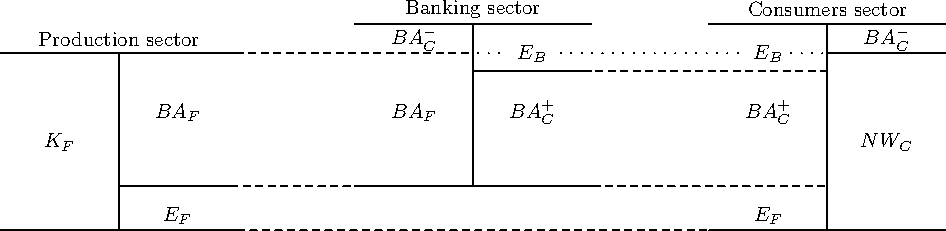
\includegraphics[scale=0.7]{manual_balances-0.pdf}
	\caption{balance sheets of the various sectors and their relationship}
	\label{fig:balances}
\end{figure}

The figure also highlights the coherence of the balance sheets and what this coherence implies. As one can easily check, the net wealth of the consumers sector ($NW_C$) is equal to production capital ($K_F$). Second, the figure shows that equities of banks and firms make up consumers wealth together with the more straightforward item represented by deposits. 

We pointed out above that the bank account is the sole financial contract in this model. The accounting is thus performed at the individual level for the wealth stored in bank accounts. Equities are not represented by shares, thus we have not a measure of individual wealth hold in shares. The amount of wealth that is represented by equity is computed at the aggregate level. These aggregate variables could be taken into account by consumers when taking decisions.   

\subsection{Technical documentation}

People who need more details can fint them in the \href{\doclocation/index_initialization.html}{technical documentation}.

\newpage
\section{The main loop}\label{sec:mainloop}
The main loop can be divided into two parts:
\begin{enumerate}
	\item the process that leads to the production of goods
	\item the process that leads to the consumption of what has been produced
\end{enumerate}
The parts of the main cycle where these two processes develop are highlighted with colors: in red the consumption process and in violet the production one. The figure also highlights which markets are interested by the two processes.

\begin{figure}[htp]
	\centering
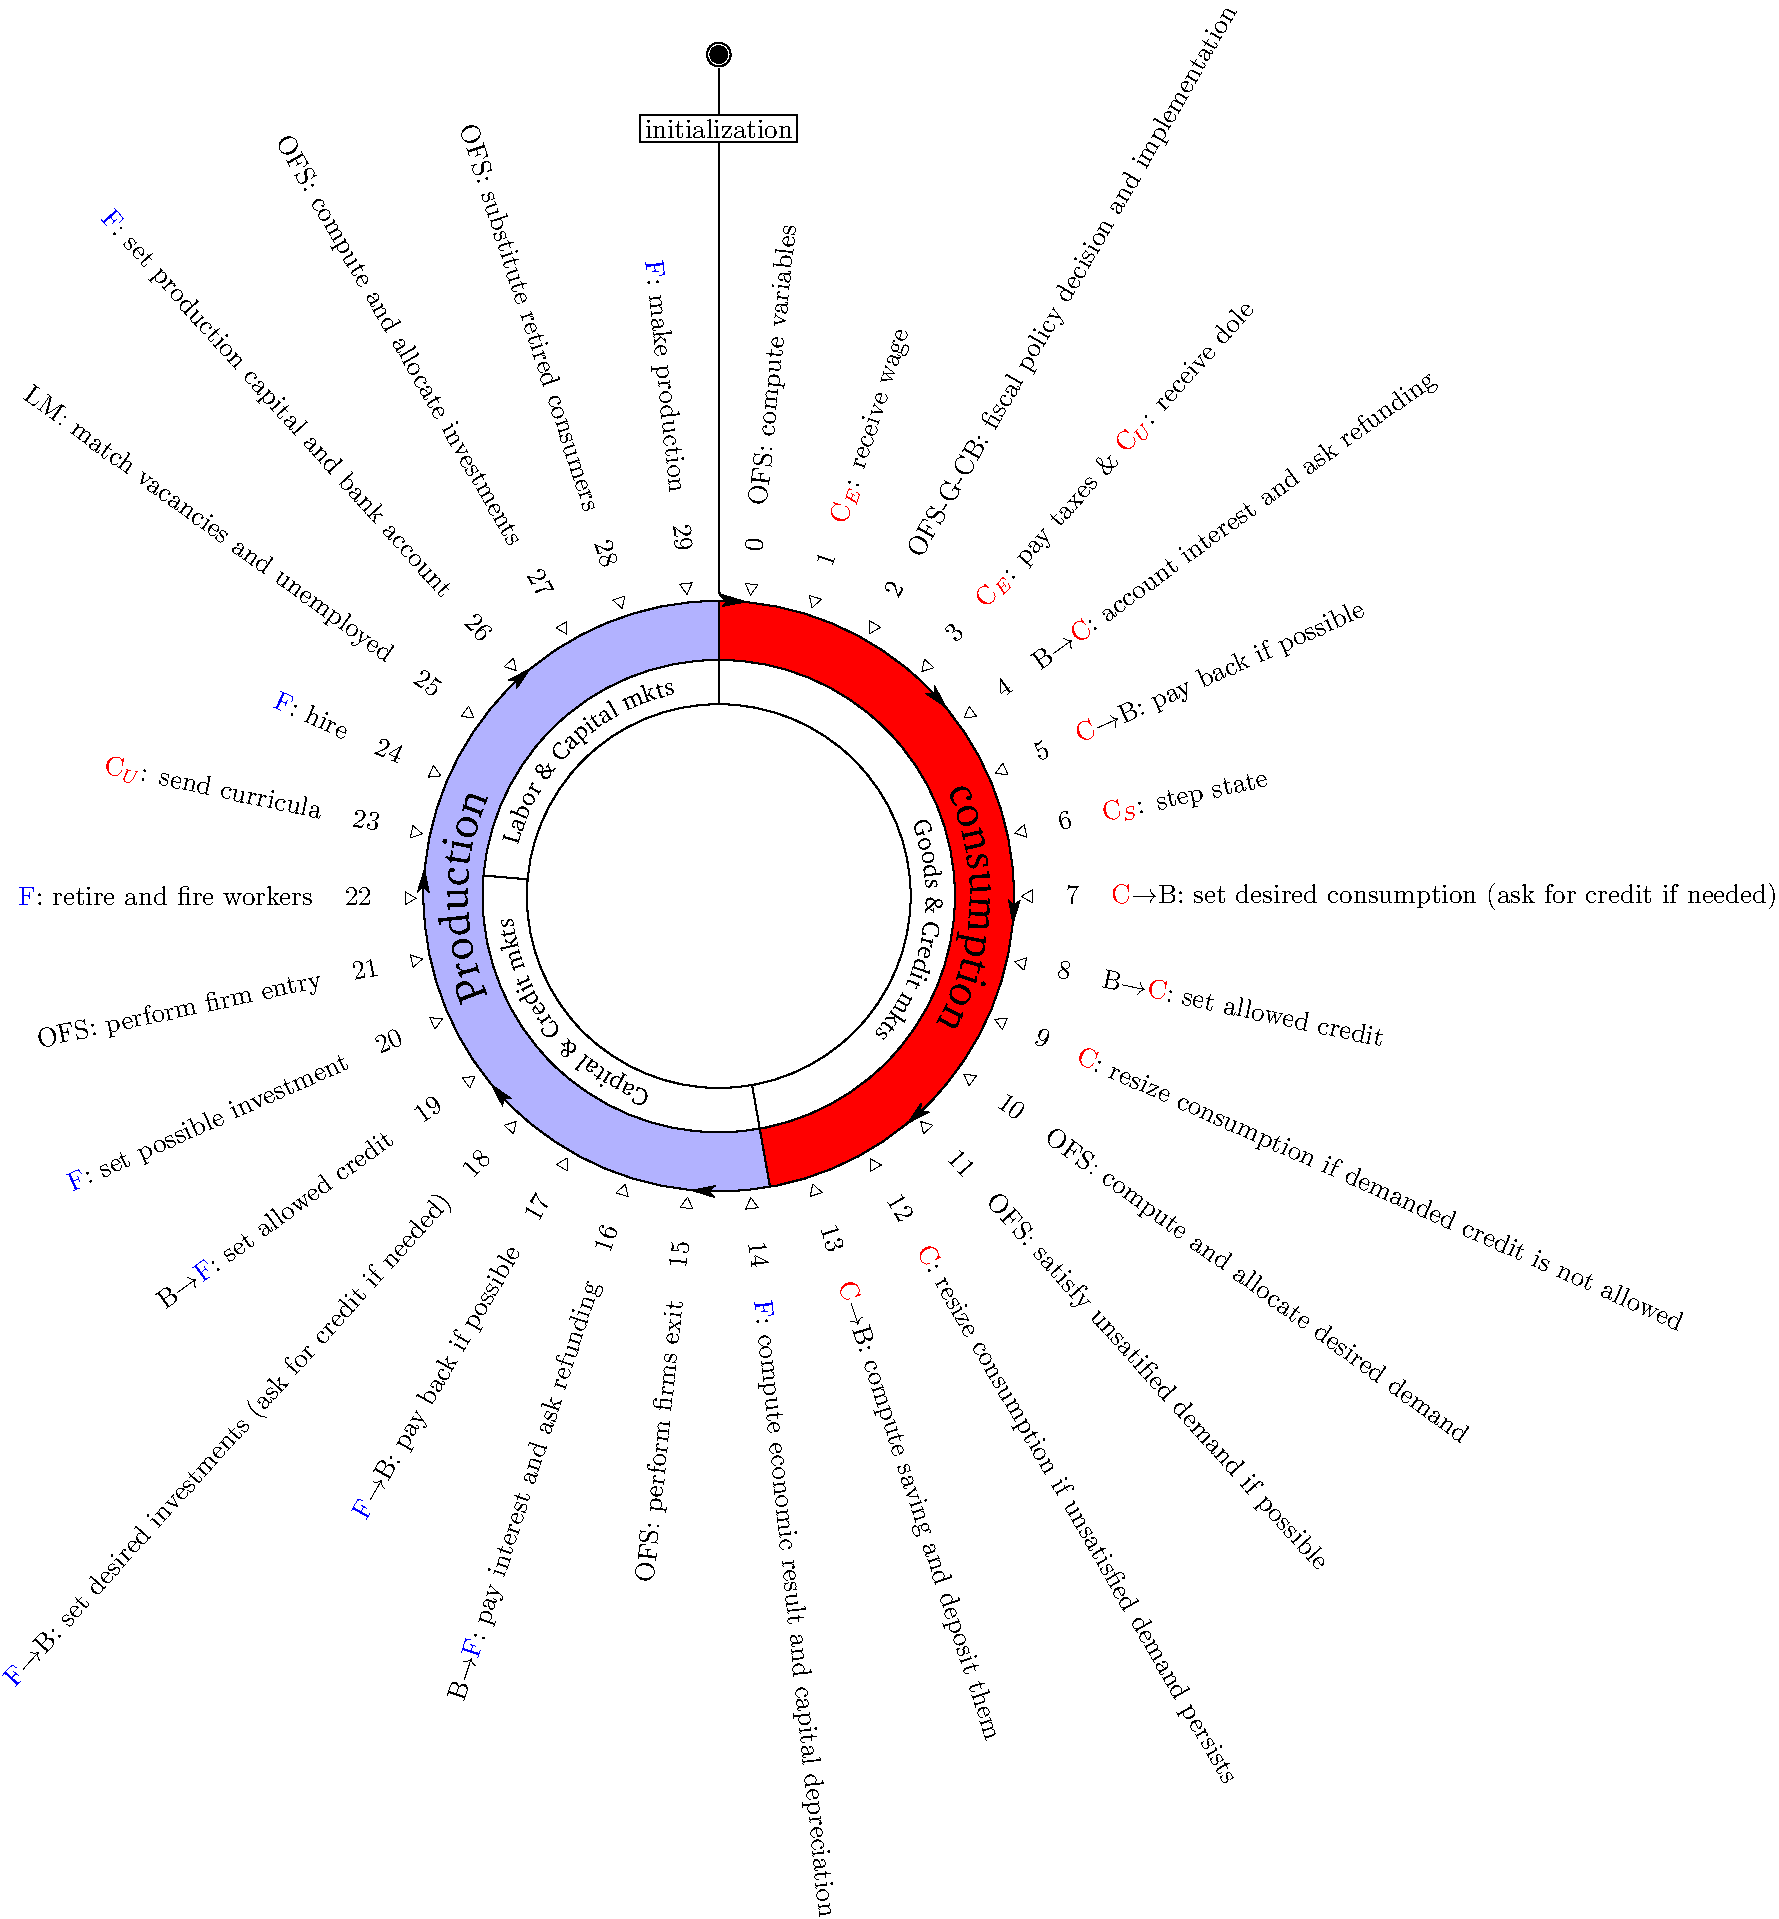
\includegraphics[scale=0.5]{visual1.pdf}
	\caption{sequence of events}
	\label{fig:clockcolor}
\end{figure}

\subsection{The process that leads to the consumption of what has been produced}
%\subsection{Consumer-market-bank relationship}
We present here the sequence of events and will enter in the details of each item in the following subsections.

The reader can easily check the correspondence between the numbering of events in figure \ref{fig:clockcolor} and that in the following list. The sequence of events is the following:
\begin{enumerate}
	\item workers receive wage;
	\item Office for statistics, Government and Central Bank implement fiscal policy
		\begin{itemize}
			\item Office for statistics provide data
			\item Central Bank sets government borrowing limit
			\item Government decides the tax rate
			\item workers pay taxes and unemployed receive the dole
			\item The government bank account at Central Bank is updated
		\end{itemize}
	\item banks 
		\begin{itemize}
			\item account interest
			\item ask for loan repayments to indebted consumers;
		\end{itemize}
	\item consumers refund if possible (if they have enough financial resources);
	\item students update their state
	\item consumers compute desired consumption and ask for credit in order to achieve the desired level 
	\item banks decide how much credit to allow;
	\item Allowed consumption is computed: consumers adjust their desired consumption according to allowed credit. 
	\item Goods markets open: Office for statistics allocate demand
	\item Office for statistic satisfies unsatisfied demand if possible.
	\item The \textit{effective} level of consumption is established: it may be less or equal to the allowed consumption.
	\item consumers adjust their bank accounts (deposits and loans) according to effective consumption.
\end{enumerate}

As for the initialization, these phases are explained in details in the \href{\doclocation/index_loop.html}{technical documentation}. There, we present the steps of the main loop in a sequential order and each step is detailed by means of an UML activity diagrams.

We will present hereafter the steps in less schematic more verbal way. In any case, the UML diagrams can be visualized by a link provided at the end of each paragraph.

\subsubsection{Consumers receive wages}

Unemployed people receive the unemployment dole (\gls{par:ud}) from the government.
The computation of workers' wage is less straightforward. The wage each employed consumer receives is a mark up on the unemployment dole: 

\begin{equation}
	\textnormal{\gls{var:ww}}=ud+\theta_{LM}\theta_{YL}f(\psi)
	\label{eq:ww}
\end{equation}
where:\\

\vskip2mm
\noindent
\begin{tabular}{l l l l}
	\hline
	& &&read\\
	notation& name &&from\\
	in equations& in code&value&file\\
	\hline
	\hline
\gls{par:ud}&\verb+Context.unemploymentDole+&30&yes\\
\gls{par:thetaLM}&\verb+Context.laborMarketStateToSetWage+&0.5&yes\\
%\gls{par:thetaYL}&\verb+Context.parameterOfProductivityInProductionFuncion+&100\\
	\hline
\end{tabular}

\vskip2mm
\gls{par:thetaYL} is the parameter of productivity in production function (already defined) and $f(\psi)$ is a function of workers' productivity.

Three possibilities for $f(\psi)$ are presently implemented:
\begin{enumerate}
	\item $f(\psi)$ is the worker's productivity;
	\item $f(\psi)$ is average productivity of workers having the worker's degree in the employer's firm;
	\item $f(\psi)$ is average productivity of workers having the worker degree in the economy.
\end{enumerate}


This leads to three different wage setting rules. One of these rules can be chosen by means of the following parameter:\\
\vskip2mm
\noindent
\begin{tabular}{l l l l}
	\hline
	& &&read\\
	notation& name &&from\\
	in equations& in code&value&file\\
	\hline
	\hline
\gls{par:wsr}&\verb+Context.wageSettingRule+&2&yes\\
	\hline
\end{tabular}

\vskip2mm
The researcher can choose which rule to use in a given run by setting the \verb+value+ of this parameter in the \verb+batch_parameters.xml+ file located in the scenario folder.
The possible values that can be specified in the parameter file are: 0, 1 and 2. Their meaning is as follows:
\begin{itemize}
	\item 
		If \verb+value=0+ the wage depends on the worker's productivity.
	\item 
		If \verb+value=1+ the wage depends on the productivity of workers employed in the firm having the same education level of the considered worker.
	\item 
		If \verb+value=2+ the wage depends on the productivity of workers having the same education level of the considered worker in the whole economy.

\end{itemize}

The UML sequence diagram of this event is available \href{\doclocation/umldoc/setWorkersWage.html}{here}.
\begin{marginfigure}
	
\includegraphics[scale=0.1]{uml.png}
\end{marginfigure}

\subsubsection{Office for statistics, Government and Central Bank implement fiscal policy}

In this step the Office for statistics, the Government and the Central Bank interact in a process that will lead each consumer to know his/her disposable income.

First of all, the Office for statistic computes the figures needed to compute the public balance: the aggregate taxable income and the aggregate dole to be payed.

Second, the central bank sets the amount of funds that is willing to borrow to the government.

Third, the government sets the tax rate that will be charged to workers, wile the unemployment dole is kept at the consumption subsistence level.

Finally, workers pay taxes and unemployed receive the dole.

\vskip5mm
\textit{\textbf{Office for statistics compute the taxable income and the number of unemployed}}

The aggregate taxable income is given by the sum of wages:
\[
TI=\sum_w w_w
\]

The number of unemployed is denoted with $U$.

\vskip5mm
\textit{\textbf{The central bank}}

First of all the Central Bank charge the interest rate on public debt:
\[
	PD=PD(1+\textnormal{\gls{var:i-}})
\]

Then, the Central Bank decides on the credit allowed to Government using the public debt-production ratio:
\[
	pd= \frac{PD}{Y}
\]

The outcome of the process can be:
\begin{itemize}
	\item $pd\uparrow$: the Government can increase the debt but the new $pd$ cannot be higher than $pd+dpd$;
	\item $pd=$: the Government cannot increase its debt;
	\item $pd\downarrow$: the Government must reduce the $pd$ at least to $pd+dpd$.
\end{itemize}
These events happen with the following probabilities:
\[
	\begin{array}{l c l}
	pr(pd\uparrow) & = &0.5 e^{-0.69pd}\\
	pr(pd=) &= &pr(pd\uparrow)\\
	pr(pd\downarrow)&=&1-pr(pd\uparrow)-pr(pd=)
	\end{array}
\]

The following table provides some numerical examples

\begin{center}
\begin{tabular}{c c c c}
	\hline
	$pd$& $pr(pd\uparrow)$ & $pr(pd=)$ & $pr(pd\downarrow)$\\
	\hline
	0   & 0.5 & 0.5 & 0\\
	0.3 & 0.4 & 0.4& 0.2\\
	0.6 & 0.33 & 0.33 & 0.33\\
	2.0 & 0.126 & 0.126 & 0.748\\
	\hline
\end{tabular}
\end{center}
It can be easily checked that the probability that the central bank finances a public deficit decreases with the level of $pd$ while the probability that the Central Bank insists on the realization of a public surplus increases with $pd$.

The outcome of the process is thus the $pd$ desired by the central bank:
\[
	pd^d=\left\{ 
		\begin{array}{l l l}
			pd+dpd& \textnormal{with probability} &pr(pd\uparrow)\\ 
			pd& \textnormal{with probability} &pr(pd=)\\ 
			pd-dpd& \textnormal{with probability} &pr(pd\downarrow)\\ 
		\end{array}
		\right.
\]

Thus, we can compute the desire public debt as
\[
PD^d=pd^dY
\]
and the desired public surplus as
\[
PD-PD^d
\]

\vskip5mm
\textit{\textbf{The government}}

The government decides the tax rate taking account of the Central Bank recommendations. However, as we will explain below, sometimes the government can oppose Central bank.
%it is willing to accommodate the central bank requests if they does not implies a sacrifice too high. In other words, the government will not set a tax rate higher than $\bar{\tau}$. 

Fist of all, the government computes the tax rate that satisfies the Central Bank recommendation by solving $\tau^d$ in the following equation:
\[
PD-PD^d=\tau^d \ TI - d \ U
\]
This gives
\[
	\tau^d= \frac{PD-PD^d+d \ U}{TI}
\]

Setting the tax rate is a little bit tricky. 
First of all, we observe that the government can always set a tax rate higher than that desired by the central bank. Because we exclude that the government increases the consumers' sacrifice, this possibility is applied only when $\tau^d<0$. In this case the government set $\tau=0$ and uses only a part of the financial resources the Central Bank is willing to lend.

In the other case, $\tau$ is set to $\tau^d$ except when $\tau^d$ is judged too high and the Government can enforce a lower tax rate. The Central bank suggestion can be opposed by rejecting its request to be refunded. Fulfilling a Central bank request of refunding, i.e. reducing the public debt, often causes an increase in the tax rate. When this increase is judged too high, the government can contain the increase by partially or totally denying The Central Bank request. In this case, an unpaid amount will be recorded for the government.

To model this possibility, we introduce a tax rate that the government would not exceed, $\bar{\tau}$. We then compute the tax rate that would prevail with no amount refunded:
\[
	\tilde{\tau}= \frac{d \ U}{TI}
\]
Note that when refunding is asked, $\tau^d>\tilde{\tau}$. Now, when $\tilde{\tau}>\bar{\tau}$ the government cannot reduce the tax rate at the desired level  $\bar{\tau}$ and it is forced to sets the tax rate to $\tilde{\tau}$.  
When $\tilde{\tau}<\bar{\tau}<\tau^d$ the government partially fulfills the Central Bank requests by setting the tax rate to $\bar{\tau}$.  

So, the tax rate is set as follows:
\[
	\tau=\left\{ 
		\begin{array}{l l l}
			0& \textnormal{if} &\tau^d<0\\ 
			\tau^d& \textnormal{if} &\tilde{\tau}>\tau^d \\ 
			\tilde{\tau}& \textnormal{if} &\bar{\tau}<\tilde{\tau}<\tau^d\\ 
			\bar{\tau}& \textnormal{if} &\tilde{\tau}<\bar{\tau}<\tau^d\\ 
		\end{array}
		\right.
\]

%Note that if $\tau^d<0$ the government , while if $\tau^d>\bar{\tau}$, the governments opposes the reduction of public debt asked by the Central Bank and does not repay all the amount asked.  
%In the remaining case, Central Banks requests are fulfilled.

\vskip5mm
\textit{\textbf{Consumers adjust to fiscal policy}}

Now, the government collects taxes and pays unemployment dole. The consumers can therefore compute their available income.

Workers' vailable income is given by $w_w(1-\tau)$.

Unemployed, receive the dole and pay no taxes, therefore their available income is equal tot he dole.

Students have no income so their available income is equal to zero.

\subsubsection{Banks account interests and ask for loan repayments}

The accounting of interest updates the households bank accounts. This is done at different interest rates according to the sign of the bank account (\gls{var:BAcb}).

Positive bank accounts are updated using the interest rate on deposits (\gls{var:i+}), so that if $BA_{cb,t}\ge 0$
\[
BA_{cb}=BA_{cb}(1+i^+)
\]

The model has two different interest rates on loans. The ordinary interest rate (\gls{var:i-}) which is charged on bank accounts with negative amount owned by workers, and the subsidized interest rate \gls{var:isub-}, charged on negative bank accounts owned by unemployed people and students. Thus, a negative bank account hold by a workers is updated as follows 
\[
BA_{cb}=BA_{cb}(1+i^-)
\]
while if the bank account belongs to a student or an unemployed we will have 
\[
	BA_{cb}=BA_{cb}(1+i^-_{sub})
\]

Once the accrued interest has been accounted, the bank may ask the reduction of some negative accounts. This involves only the accounts owned by workers.

 
The amount of a negative bank account owned by a worker desired by the bank (\gls{var:BAdb}) is determined as follows:
\[
	BA^{db}=\left\{ 
		\begin{array}{l l l}
			BA_{}(1-\theta_{is})&\textnormal{with probability}& pr_{is}\\
			BA_{}&\textnormal{with probability}& 1-pr_{is}\\
		\end{array}
		\right.
\]

The parameters involved in this computation are:

\vskip2mm
\begin{tabular}{l l l l}
	\hline
	& &&read\\
	notation& name &&from\\
	in equations& in code&value&file\\
	\hline
	\hline
	\gls{var:i+}&\verb+Context.interestRateOnDeposits+&0.001&yes\\
\gls{var:i-}&\verb+Context.interestRateOnLoans+&0.004&yes\\
\gls{var:isub-}&\verb+Context.interestRateOnSubsidizedLoans+&0.001&yes\\
\gls{par:thetais}&\verb+Context.percentageOfLoanToRefundFor+&0.1&yes\\
&\verb+          IndebtedWorkersIfAsked+&&\\
\gls{par:pris}&\verb+Context.probabilityToBeAskedToRefund+&0.5&yes\\
&\verb+          ForIndebtedWorkers+&&\\
	\hline
\end{tabular}

\vskip2mm

The UML sequence diagram of this event is available \href{\doclocation/umldoc/updateConsumersAccounts.html}{here}
\begin{marginfigure}
	
\includegraphics[scale=0.1]{uml.png}
\end{marginfigure}


\subsubsection{Consumers refund if possible}

In the previous step banks can ask to reduce amount of negative bank accounts. 

In this model households can have more than one bank account. In principle, some of them can be positive, and others negative. The downward adjustment can be asked on some of the negative accounts.  Households can face banks refunding request using all their financial assets: income (wage) and their positive bank account. 

Households first try to fulfill bank requests by moving funds from positive to negative bank accounts. If this is not enough, they use their income. However, income can be used to fulfill banks requests as long as its amount is not lower than the subsistence level of consumption. In the worst case where banks request cannot be satisfied by using all the available financial resources, the household consumes the subsistence level of consumption and the bank reduces the negative amount of the bank account by an amount lower than it would and consequently record a positive unpaid amount.     

The UML sequence diagram of this event is available \href{\doclocation/umldoc/payBackBankDebt.html}{here}
\begin{marginfigure}
	
\includegraphics[scale=0.1]{uml.png}
\end{marginfigure}

%Households first compute both the funds needed to fulfill banks requests and also computes all the available funds. Subtracting from all the available funds the subsistence level of consumption the software computes the funds that are available to satisfy banks requests.   

%If the funds available to refund are higher than the total amount needed to fulfill banks requests, all the amounts of bank accounts that was asked to be reduced are set to the amount desired by banks and the positive bank accounts are managed as follows. The first bank account of the positive bank account list is taken. If its amount is higher that the total amount to be refunded, its amount is reduced by the amount to be refunded; otherwise its amount is set to zero and the second account in the list is involved in the same process. If some amount to be refunded remains after visiting the last account of the list, the available income is used. The available income can be used to fulfill banks requests as long as its amount is not lower than the subsistence level of consumption.      


\subsubsection{Students update their states}

The evolution of a student state follows the process already described in the initialization (see page \pageref{pref:tudentevolution}).

In particular, the current period of education is successful if the new uniform random draw $u$ is less that two times the student ability:
\[
	u<2\theta_{c,as}
\]
and unsuccessful otherwise.

If the education period is successful, the number of successful years of education (\gls{var:nsye}) is increased:
\[
n_{c,sye}=n_{c,sye}+1
\]
and the degree of education is updated according to the table already reported above:
\[
	\begin{array}{l l l}
		n_{c,sye}& \textnormal{degree}& \textnormal{degree id}\\
	0\le n_{c,sye}<5 & \textnormal{none}&0\\
	5\le n_{c,sye}<8 & \textnormal{elementary}&1\\
	8\le n_{c,sye}<13 & \textnormal{intermediate}&2\\
	13\le n_{c,sye}<16 & \textnormal{college}&3\\
	16\le n_{c,sye}<18 & \textnormal{bachelor}&4\\
	18\le n_{c,sye}<21 & \textnormal{master}&5\\
	21= n_{c,sye} & \textnormal{PhD degree}&6
	\end{array}
\]
The subject's productivity is the undated as explained in the initialization section: 
\[
	\psi_c=\theta_{c,as}+\frac{0.5}{\theta_{mnpe}}n_{c,sye}
\]

The subject looses his/her state of student 
\begin{enumerate}
	\item in case of a success, if the maximum periods of possible education (\gls{par:thetamnpe} $+$ \gls{par:thetamnfpe}) or
	\item in case of failure, if the maximum number of failures admitted (\gls{par:thetamnfpe})
\end{enumerate}
is reached. In these cases, his/her status changes in unemployed.

The UML sequence diagram of this event is available \href{\doclocation/umldoc/stepStudentState.html}{here}
\begin{marginfigure}
	
\includegraphics[scale=0.1]{uml.png}
\end{marginfigure}


\subsubsection{Consumers compute desired consumption and ask for credit in order to achieve the desired level}
This task is performed by taking the following steps.

Each consumer check her/his income: workers have the wage as an income, unemployed have the dole and students have no income. Consumers also computes their financial resources by looking at their bank accounts. 

Based on this information the desired consumption is computed using a consumption function. In the current version of the model this amount is computed randomly and it can be higher or lower than the available income. 
\begin{marginfigure}
	\hskip2.5cm
\includegraphics[scale=0.2]{edit.png}
\end{marginfigure}


This allows to compute the desired total level of expenditure of consumption: \gls{var:Ddc}.

In this model we can have product differentiation. When more than one product are present, the desired demand for each item (\gls{var:Ddcj}) is computed as follows:
\[
	D_{c,j}^d=\alpha_{c,j}D^d_{c}
\]
where \gls{var:alphacj} is an index of the consumers appreciation for the given item. Of course the condition $\sum_j \alpha_{c,j}=1$ must hold.

If the available financial resources are not enough to realize desired consumption, consumers evaluate the possibility to ask for credit. This possibility is precluded if all the consumers' bank accounts have a positive unpaid amount. Otherwise, the consumer asks all the credit needed to the bank with the best bank account. 

Credit is also asked to the bank with the best bank account to satisfy unpaid amounts that exist in other banks. 


The UML sequence diagram of this event is available \href{\doclocation/umldoc/stepDesiredConsumption.html}{here}.
\begin{marginfigure}
	
\includegraphics[scale=0.1]{uml.png}
\end{marginfigure}

\subsubsection{Banks decide how much credit to allow}

In the previous step, consumers who need credit set its desired amount on one of their bank accounts (the best bank account) having null unpaid amount if such account exists. Let us identify this variable with \gls{var:BAdc} (where the $d$ upper script means \textbf desired). Because they are asking for credit, this amount is negative:  \gls{var:BAdc} $<0$. Note that the best bank account  has either a positive or a negative amount. 

In the present version of the model, the bank decides the allowed credit \gls{var:BAac} $<0$ ( superscript $a$ means \textbf allowed) as follows

\begin{itemize}
	\item if \gls{var:BAcb} $\ge 0$ and \gls{var:BAdc} $<0$
		\[BA^{a}_c=\left\{
			\begin{array}{l l l}
				BA^{d}_c&\textnormal{with probability}&pr_{ab}\\
				\theta_{ab}BA^{d}_c&\textnormal{with probability}&1-pr_{ab}\\
			\end{array}
		\right.
		\]
	\item if \gls{var:BAcb} $< 0$ and \gls{var:BAdc} $<$ \gls{var:BAcb}
		\[BA^{a}_c=\left\{
			\begin{array}{l l l}
				BA^{d}_c&\textnormal{with probability}&pr_{ab}\\
				BA_{cb}-\theta_{ab}(BA_{cb}-BA^{d}_c)&\textnormal{with probability}&1-pr_{ab}\\
			\end{array}
		\right.
		\]
\end{itemize}
This does not apply to students to whom the asked credit is always allowed.

We have thus introduced the following parameters:\\
\begin{tabular}{l l l l}
	\hline
	& &&read\\
	notation& name &&from\\
	in equations& in code&value&file\\
	\hline
	\hline
	\gls{par:thetaab}&\verb+Context.percentageOfCreditAllowedTo+&\\
 &\hskip1.5cm\verb+ConsumersWhenCreditIsNotTotallyFunded+&0.0&yes\\
 \gls{par:prab}&\verb+Context.consumersProbabilityToGetFunded+&0.5&yes\\
	\hline
\end{tabular}

\vskip3mm
The UML sequence diagram of this event is available \href{\doclocation/umldoc/setAllowedConsumersCredit.html}{here}.
\begin{marginfigure}
	
\includegraphics[scale=0.1]{uml.png}
\end{marginfigure}

\subsubsection{Consumers adjust their desired consumption according to allowed credit} 

Because there is the possibility that bank does not allow all the demanded credit, we introduce a new variable: the allowed demand (\gls{var:Dac}). 

This variable can differ from the desired demand only for consumers who asked for credit an whose request was not satisfied by banks.

Because we can have product differentiation, we first compute the allowed-desired demand ratio on the whole consumption expenditure:
\[
	r_{c}^d=\frac{D^a_c}{D^d_c}
\]
Then we scale the demand of each single item by this amount
\[
	\textnormal{\gls{var:Dacj}} =r_{c}^dD_{c,j}^d
\]

In this resizing, we do not account of unpaid amounts because we assume that credit is first used to satisfy consumption. The possible residual is then used to reduce unpaid amounts. 

The UML sequence diagram of this event is available \href{\doclocation/umldoc/adjustConsumptionAccordingToExtendedCredit.html}{here}.
\begin{marginfigure}
	
\includegraphics[scale=0.1]{uml.png}
\end{marginfigure}

\subsubsection{Good markets open: office for statistics computes and allocate desired demand and satisfy unsatisfied demand if possible}
We code the goods market functioning in such a way that both centralized and decentralized matching mechanisms can be mimicked. 
In particular, the Office for Statistic supervise the allocation of demand.

The task is performed by taking the following steps:
\begin{itemize}
	\item compute the desired allowed demand for each good type;
	\item allocate it to firms;
	\item manage unsatisfied demand;
	\item update firms sales.
\end{itemize}
These items are detailed hereafter.

\noindent$\bullet$ \textit{Compute the allowed demand for each good type.} The Office for Statistics computes the demand of each industry by summing over all the consumers. 
We mimic decentralized markets and the losses of exchange opportunities due to the matching process by introducing  the following parameter:\\


\vskip1mm
\noindent
\begin{tabular}{l l l l}
	\hline
	& &&read\\
	notation& name &&from\\
	in equations& in code&value&file\\
	\hline
	\hline
 \gls{par:thetagmi}&\verb+Context.percentageOfDemandMissed+&\\
 &\hskip1.5cm\verb+BecauseOfGoodsMarketImperfections+&0.0&yes\\
	\hline
\end{tabular}

\vskip3mm
The demand of industry producing item $j$ is therefore computed as follows:
\[
	\textnormal{\gls{var:Dajc}}=(1-\theta_{gmi})\sum_c  \textnormal{\gls{var:Dacj}}
\]
where the $\leftarrow c$ signal that demand comes from consumers. This notation allows to identify the various sources of demand that will be introduced below in the text and in future extensions. 

Provided that in the economy there are $J$ industries, the software computes an array of dimension $J$: $\{D^a_{1\leftarrow c},\cdots,D^a_{J\leftarrow c}\}$.

The desired allowed aggregate demand is also computed:
\[
	D^a_{\leftarrow c}=\sum_j\textnormal{\gls{var:Dajc}}
\]

The UML sequence diagram of this event is available \href{\doclocation/umldoc/computeDesiredDemand.html}{here}.
\begin{marginfigure}
	
\includegraphics[scale=0.1]{uml.png}
\end{marginfigure}

\noindent$\bullet$ \textit{Allocate desired allowed demand to firms.} In this step, the demand computed in the previous step (\gls{var:Dajc}) is allocated to the various firms according to their share of production in the industry they belong to:
\begin{equation}
	\textnormal{\gls{var:Dafjc}}=\textnormal{\gls{var:Dajc}}\frac{\textnormal{\gls{var:Yfjc}}}{\textnormal{\gls{var:Yjc}}}
	\label{eq:Dafjc}
\end{equation}
It will be clarified in the \verb+make production+ step that firms produce goods that are sold to other firms (\gls{var:Yfjf}) to let them adjust their production capital and consumption good sold to consumers (\gls{var:Yfjc}). The just written computation involves the latter.
 
The specific step we are discussing allows firms to know the appreciation of the item they produce among consumers. 
Note that firms in some industries may be in a short supply situation (\gls{var:Dajc} $>$ \gls{var:Yfjc}) while in other industries the opposite may hold. This information will be used by firms to guide their production choices.

The UML sequence diagram of this event is available \href{\doclocation/umldoc/allocateDesiredDemand.html}{here}.
\begin{marginfigure}
	
\includegraphics[scale=0.1]{uml.png}
\end{marginfigure}

\noindent$\bullet$ \textit{Manage unsatisfied demand.} In this model we have vertical differentiation. This means that products with higher $j$ are more advanced and, therefore, preferred. It may thus happen that demand on these product is higher than supply. 
In case the demand of a given product cannot be entirely satisfied, the office for statistics try to fulfill consumers excess demand of this product with the product that precede it in the quality ladder. The Office for statistic moves demand across industries starting from the most advanced product and proceeding backward. 
This mechanism aims to mimic consumer decision to buy a less advanced product if the item s/he desires is in short supply.

At the end of this process the demand received by each industry (\gls{var:Dj}) and that received by each firm (\gls{var:Dfj}) is known.

Consumers are then informed of the demand reallocation and their final demand is computed:
\[
	\textnormal{\gls{var:Dcj}}= \textnormal{\gls{var:Dacj}}\frac{\textnormal{\gls{var:Dj}}}{\textnormal{\gls{var:Dajc}}}
\]

The UML sequence diagram of this event is available \href{\doclocation/umldoc/matchDemandAndSupply.html}{here}.
\begin{marginfigure}
	
\includegraphics[scale=0.1]{uml.png}
\end{marginfigure}


\noindent$\bullet$ \textit{Update firms sales.}
Firms are also informed on the items they have sold:
\[
	\textnormal{\gls{var:Dfj}}=\textnormal{\gls{var:Dj}}  \frac{\textnormal{\gls{var:Yfjc}}}{\textnormal{\gls{var:Yjc}}}
\]
This information will be then used to compute profit.

Two UML sequence diagrams describe this event. \begin{marginfigure}
	
\includegraphics[scale=0.1]{uml.png}
\end{marginfigure}
The first one describe the computation performed by the office for statistics of the demand starting from the consumer data. This allows a double check on the computation of \gls{var:Dj} an is available \href{\doclocation/umldoc/computeDemand.html}{here}. The second one describes the allocation of demand to firms and is available \href{\doclocation/umldoc/allocateDemand.html}{here}.

\subsubsection{Consumers adjust their bank accounts (deposits and loans) according to effective consumption}
Summing up, in this model the desired consumption can be resized two times. The first one when the consumer asks for credit to achieve its desired consumption, but the bank does not allow the demanded credit. In this case we have that the allowed consumption (\gls{var:Dac}) is lower than desired consumption (\gls{var:Ddc}). The second one is when the asked good is in short supply. In this case, we say that the effective consumption (\gls{var:Dc}) is lower than the allowed consumption (\gls{var:Dac}). The effective consumption is computed as follows:
\[
\textnormal{\gls{var:Dc}}=\sum_j \textnormal{\gls{var:Dcj}}
\]

Once the effective consumption is known, consumers pay the due amounts to firms.
The consumers financial position is adjusted accordingly.
Those who consumes less that their income brings their saving to the bank with the worst position. Those who were allowed credit decrease their best bank account by the amount needed to consume. If additional allowed credit remains, it is used to reduce or cancel the unpaid amounts possibly present in the other bank accounts.   

The UML sequence diagram of this event is available \href{\doclocation/umldoc/updateBankAccountAccordingToEffectiveConsumption.html}{here}.
\begin{marginfigure}
	
\includegraphics[scale=0.1]{uml.png}
\end{marginfigure}

\subsection{Example of consumer-banks relationship}

A numerical example of the sequence of action of the above explained process is given hereafter.% can be reached by clicking \href{\doclocation/latexdoc/example_consumer_bank_relationship.html}{here}
\begin{marginfigure}
\hskip8mm	
\includegraphics[scale=0.07]{example.png}
\end{marginfigure}

The focus is on an indebted Consumer.

We trace hereafter the steps explained in the manual.  
%\subsubsection*{Step 1: interests and ask for repayments}
\subsubsection*{Step 1: interests and loans repayment}

In this example, each consumer is customer of three banks.

First of all, banks account the interest rate.

Suppose that after accounting interest rate, the consumer's bank accounts have the following amounts:
\begin{verbatim}
bank 1 account =   10
bank 2 account = -150
bank 3 account =  -50
\end{verbatim}

The bank assumes that indebted consumers (those with a negative bank account) ask for the whole renewal of the debt:

\begin{verbatim}
bank 1 account =   10  demanded credit =    0
bank 2 account = -150  demanded credit = -150
bank 3 account =  -50  demanded credit =  -50
\end{verbatim}

Each bank with a negative account can ask for refunding. If this happens, the allowed credit is lower (in absolute value) than the demanded credit.
Suppose banks 2 and 3 intend to reduce their exposition as follows:

\begin{verbatim}
bank 1 account =   10  demanded credit =    0 allowed credit =    0
bank 2 account = -150  demanded credit = -150 allowed credit = -130 
bank 3 account =  -50  demanded credit =  -50 allowed credit =  -45
\end{verbatim}

In this example, the consumer needs 25 to satisfy banks requests.

\subsubsection*{step 2: refunding}
The consumer refunds her bank account if she has enough income (to refund) and, in any case, refunds an amount that allows a subsistence consumption level. 
\\Let's consider this example:

\verb+disposableIncome=40+\\
and that the subsistence consumption is 10.

The software first computes the resources available to refund. They are given by 
the sum of positive amounts in bank accounts plus the disposable income minus the subsistence consumption. In this example we have:

\verb/resourceAvailableToRefund = 10 + 40 - 10 = 40/

These resources are enough to satisfy banks' requests; the consumer refunds totally banks because her financial resources allow both debt repayment and a consumption greater than the subsistence level. 
Therefore, the new situation is:

\begin{verbatim}
bank 1 account =   10  demanded credit =    0 allowed credit =    0
bank 2 account = -130  demanded credit = -150 allowed credit = -130 
bank 3 account =  -45  demanded credit =  -50 allowed credit =  -45

disposableIncome = 15
\end{verbatim}


%If the income is not enough to refund and have the minimum consumption, the consumers makes a proposal to the bank by reducing the demand for credit. 

Consider now a slightly different situation in bank accounts:
\begin{verbatim}
bank 1 account =   15  demanded credit =    0 allowed credit =    0
bank 2 account = -150  demanded credit = -150 allowed credit = -130 
bank 3 account =  -50  demanded credit =  -50 allowed credit =  -45
\end{verbatim}
the only difference with the previous situation is that the amount in bank 1 is 15 instead of 10.
Suppose furthermore that the consumer's income is 15 instead of 40. Now resources available to refund banks (the sum of positive amounts in bank accounts plus the disposable income minus the subsistence consumption) are given by:

\verb/resourceAvailableToRefund = 15 + 15 - 10 = 20/

They are not enough to satisfy banks' requests (25 is needed). Suppose 15 is used to refund bank 1 and 5 to refund bank 2. Unpaid amounts are recorded and disposable income is set to allow the subsistence consumption:

\begin{Verbatim}[commandchars=\\\{\}]
bank 1: account =    {\bf0}  demanded credit =    0 allowed credit =    0 unpaid =  0
bank 2: account = -135  demanded credit = -150 allowed credit = -130 unpaid =  5
bank 3: account =  -50  demanded credit =  -50 allowed credit =  -45 unpaid =  5

disposableIncome = {\bf10}
\end{Verbatim}

We continue this example with this second situation.

\subsubsection*{Step 3: account resetting}
In this step, banks set the demanded and allowed credit to zero.

Banks accounts are the updated as follows:

\begin{Verbatim}[commandchars=\\\{\}]
bank 1: account =    0  demanded credit =  0 allowed credit = 0 unpaid =  0
bank 2: account = -135  demanded credit =  {\bf0} allowed credit = {\bf0} unpaid =  5
bank 3: account =  -50  demanded credit =  {\bf0} allowed credit = {\bf0} unpaid =  5

disposableIncome = 10
\end{Verbatim}




\subsubsection*{step 4: consumers set desired credit}
Now each consumer can asks for new credit. This can be done for two reasons: 1) to achieve a desired consumption higher than disposable income and 2) to pay unsatisfied lenders.

Suppose now that the consumer would like to consume 20.

She asks for additional financial resources both to finance consumption (10) and to pay back bank 2 and 3 (5+5).

The additional credit amount of 20 is asked to one bank. In particular, the bank with the ``best'' account (bank 1) is chosen. 

\begin{Verbatim}[commandchars=\\\{\}]
bank 1: account =    0  demanded credit = {\bf-20} allowed credit = 0 unpaid =  0
bank 2: account = -135  demanded credit =   0 allowed credit = 0 unpaid =  5
bank 3: account =  -50  demanded credit =   0 allowed credit = 0 unpaid =  5

disposableIncome = 10  desiredConsumption = 20
\end{Verbatim}


\subsubsection*{Step 5: credit supply}

%The bank decides how much credit to allow.

The bank decides about the amount of loans to give out.
Suppose allowed credit is 18

\begin{Verbatim}[commandchars=\\\{\}]
bank 1: account =    0  demanded credit = -20 allowed credit = {\bf-18} unpaid =  0
bank 2: account = -135  demanded credit =   0 allowed credit =   0 unpaid =  5
bank 3: account =  -50  demanded credit =   0 allowed credit =   0 unpaid =  5

disposableIncome = 10  desiredConsumption = 20
\end{Verbatim}

Note that the funds now available to the consumers are 

\verb\disposableIncome + allowed credit=10+18=28\ 

\subsubsection*{step 6: adjust desired consumption according to allowed credit}

In this step, the allowed consumption is introduced and it is given by the difference between the demanded and the allowed credit. In any case, the allowed consumption cannot be lower than the subsistence level.

In the example we have

\begin{Verbatim}[commandchars=\\\{\}]
bank 1: account =    0  demanded credit = -20 allowed credit = -18 unpaid =  0
bank 2: account = -135  demanded credit =   0 allowed credit =   0 unpaid =  5
bank 3: account =  -50  demanded credit =   0 allowed credit =   0 unpaid =  5

disposableIncome = 10 desiredConsumption = 20 allowedConsumption = {\bf18}
\end{Verbatim}

Now, the consumer goes in the goods market trying to satisfy her desired-allowed consumption. It may happen that goods are in short supply. Suppose this is the case and she can buy 15 instead of 18. 

\subsubsection*{step 7: the consumer adjust bank accounts}

The consumer can thus consume 15. 10 of them are payed with disposable income and 5 of them are borrowed from bank 1. 

Bank 1 is also willing to lend additional resources (18-5=13), so the consumer uses them to satisfy bank 2 and 3 refunding requests:

\begin{Verbatim}[commandchars=\\\{\}]
bank 1: account =  {\bf-15}  demanded credit = -20 allowed credit = -18 unpaid =  0
bank 2: account = -130  demanded credit =   0 allowed credit =   0 unpaid =  {\bf0}
bank 3: account =  -45  demanded credit =   0 allowed credit =   0 unpaid =  {\bf0}

disposableIncome = {\bf0}  desiredConsumption = 20 allowedConsumption = 18 
                                              effectiveConsumption = 15
\end{Verbatim}




\subsection{The process that leads to production}

The bulk of this process consists in firms' attempt to adjust inputs to be able to make the production needed to satisfy the demand expected for the next period.

First of all, firms have to decide the level of production to be realized in the next period. To this aim, they have two important signals from the present period: the level of desired demand from consumers and that from other firms (the latter relates to investment as we will clarify below).
Concerning the demand from consumers, we recall that the quantity sold by a firm can be different from that initially demanded by consumers. Indeed, the discussion in the previous section points out that when a consumer does not find enough goods of a given type, her/his demand is moved
%can be moved (depending the chosen parametrization) 
to other goods.
%by the Office For Statistic. 
However, the firm is informed on the initial level of demand (that desired by consumers) on the item it produces. It is thus natural a firm would realize a production equal to the demand initially claimed by consumers.  

%This information is used to set the target level of production. Once this figure has been established, the firm starts the inputs adjustment process in order to achieve the production target. 

Inputs already available to the firm can be higher or lower than those needed to realize the target production. Inputs excesses are someway easier to manage than shortages: workers can be fired while a part of the available production capital can stay unproductive.
The upward adjustment is instead more tricky because 
%the joint availability of resources must be checked.
%Both production capital and labor force are involved in the adjustment. S
several impediments to reach the desired level of inputs can occur.
The level of financial resources, including new available credit, can be the first constraint to the inputs increase. The availability of the inputs on the market is a second constraint. Finally, if one of these constraints is binding for one of the inputs, the demand of the others must be adjusted coherently. Inputs shortages deserves additional care by making a distinction between inputs that can be produced and those whose production is not possible or cannot be easily obtained in the short run. 

\label{pg:inputs2}
As already mentioned above, in the present version of the model we have two inputs: production capital and labor. We treat production capital as ``producible'' while labor as non producible. So when a production capital shortage is detected, it can be produced to satisfy the shortage. However, the model checks for the existence of unused production capital before new production capital is asked.
Production capital, as labor, preserves (in full or in part) its production power when it is moved to another firm. %for the future even if it is not employed in a given period. 
We account for this by including a market for existing unused production capital. So, firms that needs additional production capital, first try to buy already existing production goods that are not used by other firms. Firms that after this adjustment still needs production capital ask for new production goods to other firms. To keep the model simple, we assume that production goods are made up of the same goods available to consumers, so that, at the end, new investments affect the demand on the existing goods markets.


%So, the firm has first to check how many financial resources are available for realizing the desired investment. Then It has to check if there are enough unemployed labor force available. Once the new realizable production is known the production factor adjustment starts: workers are hired and production capital is bought. Concerning the latter, the firm first buys existing unused production capital if it exists. If, after this adjustment the firm 

The actions leading to production are numerous and not so straightforward. To ease the understanding of their unfolding it is convenient to refer to the violet part of figure \ref{fig:clockcolor}. We also report them hereafter as a list. We provide the reader with a ``coarse grain'' description with the gray backgrounded items.

\begin{itemize}
%	\item set the target level of production
	\item \colorbox{lightgray}{check available financial resources} for upward adjustment of production capital. This phases is performed by taking the following steps:

\begin{enumerate}
		\setcounter{enumi}{11}
	\item compute the economic result and capital depreciation;
	\item perform firms exit;
	\item banks account interests and ask for loan repayments to indebted firms;
	\item firms refund if possible;
	\item firms step the product innovation process;
	\item[- - ] the software performs a technical step by resetting some variables of the bank accounts;
	\item firms ask for new credit;
	\item banks decide how much credit to allow;
	\item firms compute investment demand and supply and adjust unpaid amount if possible.
	\item entry of new firms that will ask for production capital.
\end{enumerate}


	\item \colorbox{lightgray}{Labor force adjustment} taking in mind the possible financial constraints
		\begin{enumerate}
		\setcounter{enumi}{19}
			\item Firms perform labor force downward adjustment;
			\item Unemployeds send curricula;
			\item Perform labor force upward adjustment using decentralized matching; 
			\item Perform labor force upward adjustment using centralized matching; 
		\end{enumerate}
%	\item The firm can be constrained in the labor market, thus the available financial resources can remain partially unused. The entrepreneur lines up the production capital coherently with the gathered workforce.  
	\item \colorbox{lightgray}{Production capital adjustment} taking in mind the possible workers constraint
		\begin{enumerate}
		\setcounter{enumi}{23}
			\item Firms try to adjust their production capital on the market for used production capital;
			\item Firms that need additional capital ask for new production goods;
		\end{enumerate}
	\item \colorbox{lightgray}{Consumer turnover}
		\begin{enumerate}
		\setcounter{enumi}{25}
			\item perform consumers turnover
		\end{enumerate}
	\item \colorbox{lightgray}{Make production}
		\begin{enumerate}
		\setcounter{enumi}{26}
			\item firms make production
		\end{enumerate}


\end{itemize}

We will now enter into details of each step. The gray backgrounded headings will signal when the detailed description leaves one group to enter the next group of actions.

\subsection*{\colorbox{lightgray}{Check available financial resources}}
\subsubsection{Compute the economic result and capital depreciation}
Each firm economic result (\gls{var:pifj}) is computed as follows

\[
	\textnormal{\gls{var:pifj}} =\textnormal{\gls{var:Dfj}}+\textnormal{\gls{var:Dff}}-\textnormal{\gls{var:Wfj}}
\]
where \gls{var:Dfj} is demand from consumers, \gls{var:Dff} is demand from firms and \gls{var:Wfj} is the amount of wages payed by the firm.

\gls{var:Wfj} is the sum of the individual wage (\gls{var:ww}) payed by the firm to the workers it employs. We saw above how \gls{var:ww} is computed (see equation \ref{eq:ww}), so we can write
\[
	\textnormal{\gls{var:Wfj}}=\sum_{w \ \textnormal{in} \ f} \textnormal{\gls{var:wwf}}
\]


Profit (a positive economic result) can be used to buy production capital if needed. To see if profit is to be used to buy production capital, we have to update the state of this variable taking account of its depreciation.

The production capital of the firm is denoted with \gls{var:Kf}. We divide this amount into two parts: the production capital that was employed in the production and that which is in excess (if any). Remembering the production function, the production capital used in the production is  \gls{var:Yfj} and the unused part (if any) is \gls{var:Kf} $-$ \gls{var:Yfj}.


In this model, these two parts of production capital have two distinct depreciation rate \gls{par:thetadrD} and \gls{par:thetadrU}.

The production capital is thus updated as follows:
\[
	K_f=Y_{f,j}(1-\theta_{drD})+(K_f-Y_{f,j})(1-\theta_{drU})
\]

We have thus defined the following parameters\\

\noindent
\begin{tabular}{l l l l}
	\hline
	& &&read\\
	notation& name &&from\\
	in equations& in code&value&file\\
	\hline
	\hline
 \gls{par:thetadrD}&\verb+Context.percentageOfUsedCapitalDepreciation+&0.01&yes\\
 \gls{par:thetadrU}&\verb+Context.percentageOfUnusedCapitalDepreciation+&0.0&yes\\
	\hline
\end{tabular}

\vskip3mm



The UML sequence diagram of this event is available \href{\doclocation/umldoc/computeEconomicResultAndCapitalDepreciation.html}{here}.
\begin{marginfigure}
	
\includegraphics[scale=0.1]{uml.png}
\end{marginfigure}


\subsubsection{Perform firms exit}

In this basic version of the model, firms turnover is very simple: each firm that becomes too small is replaced with a new firm.
\begin{marginfigure}
	\hskip2.5cm
\includegraphics[scale=0.2]{edit.png}
\end{marginfigure}

In particular, the exit condition is
\[
	\textnormal{\gls{var:Dfj}}+\textnormal{\gls{var:Dfj}}<\textnormal{\gls{par:Dexit}}
\]

where we use the following parameter 

\noindent
\begin{tabular}{l l l l}
	\hline
	& &&read\\
	notation& name &&from\\
	in equations& in code&value&file\\
	\hline
	\hline
\gls{par:Dexit}&\verb+Context.thresholdDemandForFirmsExit+&20&yes\\
	\hline
\end{tabular}

\vskip3mm


In this part of the code, the list of new entrants is created but firms are not yet included in the model. This is because new entrants have to participate in the production factor markets in order to start the production. % Note that in the previous step, incumbent prepared for the adjustment of production capital. Thus, 
The demand for production capital that will be computed below will account for the demand of both incumbent and new firms. This will also apply to the labor demand.

The UML sequence diagram of this event is available \href{\doclocation/umldoc/performFirmsExit.html}{here}.
\begin{marginfigure}
	
\includegraphics[scale=0.1]{uml.png}
\end{marginfigure}

\subsubsection{Banks account interests and ask for loan repayments to indebted firms}

The accounting of interest updates the firms bank accounts.

Positive bank accounts are updated using the interest rate on deposits \gls{var:i+}, so that if \gls{var:BAfb} $\ge 0$
\[
BA_{fb}=BA_{fb}(1+i^+)
\]

Differently from consumers, firms have not a subsidized interest rate, and negative bank accounts are charged by the ordinary interest rate (\gls{var:i-}):
\[
BA_{fb}=BA_{fb}(1+i^-)
\]

Once the accrued interest has been accounted, the bank may ask the reduction of some negative accounts.
The amount of a negative bank account owned by a firm desired by the bank is thus determined as follows:
\[
	\textnormal{\gls{var:BAdb}} =\left\{ 
		\begin{array}{l l l}
			BA_{fb}&\textnormal{with probability}& pr_{fbren}\\
			BA_{fb}\theta_{fbncr}&\textnormal{with probability}& 1-pr_{fbren}\\
		\end{array}
		\right.
\]

The parameters involved in this computation are:

\vskip2mm
\noindent
\begin{tabular}{l l l l}
	\hline
	& &&read\\
	notation& name &&from\\
	in equations& in code&value&file\\
	\hline
	\hline
\gls{par:thetafbncr}&\verb+Context.percentageOfOutstandingCreditAllowedTo+&\\
&\hskip1.5cm\verb+FirmsWhenCreditIsNotCompletelyRenewed+&0.9&yes\\
\gls{par:prfbren}&\verb+Context.firmsProbabilityToHaveOutstanding+&\\
&\hskip3cm\verb+DebtCompletelyRenewed+&0.5&yes\\
	\hline
\end{tabular}

\vskip3mm

The UML sequence diagram of this event is available \href{\doclocation/umldoc/updateFirmsAccounts.html}{here}
\begin{marginfigure}
	
\includegraphics[scale=0.1]{uml.png}
\end{marginfigure}


\subsubsection{Firms refund if possible}
In the previous step banks can ask firms to reduce amount of negative bank accounts. 

In this model firms can have more than one bank account. In principle, some of them can be positive, and others negative. The downward adjustment can be asked on some of the negative accounts.  Firms can face banks refunding requests using all their financial assets: cash flow and their positive bank account. 

In case refund is asked on some accounts, the entrepreneur starts checking its bank account list from the beginning and when s/he find a positive amount use it to fulfill the other banks refunding requests.
If the positive amounts are not enough, the cash on hand is used. If Even cash on hand is not enough, a positive unpaid amount is recorded.

The UML sequence diagram of this event is available \href{\doclocation/umldoc/firms_payBackBankDebt.html}{here}
\begin{marginfigure}
	
\includegraphics[scale=0.1]{uml.png}
\end{marginfigure}

\subsubsection{Firms step the product innovation process}

Innovation in this model comes into the form of product innovations. We model this process by introducing the variable \gls{var:ARf} which denotes the Absolute Rank of the good produced by firm $f$.  
\gls{var:ARf} gives the position of the good in the quality ladder where higher values denote higher quality.

The product innovation is implemented in a very simple way\begin{marginfigure}\hskip23mm
	
\includegraphics[scale=0.2]{edit.png}
\end{marginfigure}


\[
	\textnormal{\gls{var:ARf}} =\left\{ 
		\begin{array}{l l l}
			AR_{f}+1&\textnormal{with probability}& pr_{pi}\\
			AR_{f}&\textnormal{with probability}& 1-pr_{pi}\\
		\end{array}
		\right.
\]

The parameters involved in this computation is:

\vskip2mm
\noindent
\begin{tabular}{l l l l}
	\hline
	& &&read\\
	notation& name &&from\\
	in equations& in code&value&file\\
	\hline
	\hline
\gls{par:prpi}&\verb+Context.probabilityOfAProductInnovation+&0.0&yes\\
	\hline
\end{tabular}

\vskip3mm
The UML sequence diagram of this event is available \href{\doclocation/umldoc/stepProductInnovatioProcess.html}{here}
\begin{marginfigure}
	
\includegraphics[scale=0.1]{uml.png}
\end{marginfigure}




\vskip3mm
We saw above that the office for statistics allocate demand. In doing that it accounts for goods quality: higher quality attracts more demand.
%The assumption is that the demand of a products depends on its quality. In this way, products with low quality are not demanded and 
This implies that firms that do not innovate are penalized. This can lead less advanced products to disappear. 

As time passes, a \gls{par:prpi} $>0$ implies that absolute ranks of the products that are exchanged in the economy always increase. Because low ranked goods disappear, we introduce the Relative Rank  \gls{var:RRf} to perform computation. It is defined as:
\[
RR_f=AR_f-\min(AR_f)+1
\]



In this way, even if the absolute rank of the less advanced good that is exchanged at a given time ($\min(AR_f)$) increases, its relative rank is alway 1.

Consider for example companies producing smart phones. Suppose we identify these companies with uppercase letters A, B, C and so on. Suppose furthermore that they name their product by the company name and the absolute rank of the product. Suppose the variety of smart phones available on the market is A6, B6, C5. We can compute the relative rank as explained above. The following table reports the situation
\begin{center}
\begin{tabular}{c c c c}
	\hline
	$f$ & product & $AR_f$ & $RR_f$\\
	\hline
	A & A6 & 6 & 2\\
	B & B6 & 6 & 2\\
	C & C5 & 5 & 1\\
	\hline
\end{tabular}
\end{center}

Suppose company A launches its new A7 smart phone. The previous table evolve as follows
\begin{center}
\begin{tabular}{c c c c}
	\hline
	$f$ & product & $AR_f$ & $RR_f$\\
	\hline
	A & A7 & 7 & 3\\
	B & B6 & 6 & 2\\
	C & C5 & 5 & 1\\
	\hline
\end{tabular}
\end{center}

After the introduction of this new product, consumers see C5 outdated. So company C either exits from the market or succeeds in innovating and launches the C6. In both cases, the relative rank is updated: 
\begin{center}
\hskip1cm if C exits \hskip5cm if C innovates

\begin{tabular}[t]{c c c c}
	\hline
	$f$ & product & $AR_f$ & $RR_f$\\
	\hline
	A & A7 & 7 & 2\\
	B & B6 & 6 & 1\\
	\hline
\end{tabular}
\hskip2cm
\begin{tabular}[t]{c c c c}
	\hline
	$f$ & product & $AR_f$ & $RR_f$\\
	\hline
	A & A7 & 7 & 2\\
	B & B6 & 6 & 1\\
	C & C6 & 6 & 1\\
	\hline
\end{tabular}

\end{center}



\subsubsection{Firms ask for new credit}

Firms may need new credit to increase the level of their production capital or to pay residual unpaid amounts on banks accounts.

First, a firm evaluates if it has to increase its production capital. In doing that it has to forecast the level of next period demand. We know there are two sources of demand: from consumers and from firms. To forecast the consumers demand, the firm uses the desired-allowed demand \gls{var:Dafjc} as computed in equation \ref{eq:Dafjc}.   
The demand from other firms is assumed to be equal to that received in the previous period. The demand expected by the firm is thus
\[
	\textnormal{\gls{var:Def}}=\textnormal{\gls{var:Dafjc}}+\textnormal{\gls{var:Dfjf}}
\]
Now, remembering the production function, we have that the desired level of production capital is:
\[
	\textnormal{\gls{var:Kdf}}=\textnormal{\gls{var:Def}}
\]
If 
\[
\textnormal{\gls{var:Kdf}}>\textnormal{\gls{var:Kf}}
\]
financial resources are needed to make the desired adjustment. The firm checks its internal financial resources, i.e. cash on hand and positive bank accounts and, if they are not enough, asks for credit. 

If existing production capital is enough to produce the expected demand, credit could be also needed; this happen if unpaid amounts exist.

If credit is needed, the entrepreneur checks the possibility to ask it to the banks it is customer of. This possibility is prevented if positive unpaid amount are present in all the firm's bank accounts. If one or more bank accounts have no unpaid amount, the entrepreneur choses the bank account having the best account to ask new credit. 
%Because all the bank accounts are evaluated by all firms, t
When searching for the best bank account, the code also identifies the worst bank; it will be used to deposit the residual cash on hand that possibly remains at the end of the adjustment process. 

The UML sequence diagram of this event is available \href{\doclocation/umldoc/setDesiredCredit.html}{here}
\begin{marginfigure}
	\includegraphics[scale=0.1]{uml.png}
\end{marginfigure}

\subsubsection{Banks decide how much credit to allow}

In the previous step, firms who need credit set the desired amount on one (the best) of their bank accounts having null unpaid amount if such account exists. Let us identify this variable with \gls{var:BAdf} (where the $d$ upper script means \textbf desired). Because they are asking for credit, this amount is negative: \gls{var:BAdf} $<0$. Note that the best bank account con have either a positive or negative amount. 

In the present version of the model, the bank decides the allowed credit \gls{var:BAabf} $<0$ (\textbf allowed by \textbf bank to \textbf firm) as follows

\begin{itemize}
	\item if \gls{var:BAfb} $\ge 0$ and \gls{var:BAabf} $<0$
		\[\textnormal{\gls{var:BAabf}} =\left\{
			\begin{array}{l l l}
			\textnormal{\gls{var:BAdf}}&\textnormal{with probability}&\textnormal{\gls{par:prabf}}\\
			\textnormal{\textnormal{\gls{par:thetaabf}}\gls{var:BAdf}}&\textnormal{with probability}&1-\textnormal{\gls{par:prabf}}\\
			\end{array}
		\right.
		\]
	\item  if \gls{var:BAfb} $< 0$ and \gls{var:BAabf} $<0$
		\[\textnormal{\gls{var:BAabf}} =\left\{
			\begin{array}{l l l}
			\textnormal{\gls{var:BAdf}}&\textnormal{with probability}&\textnormal{\gls{par:prabf}}\\
			\textnormal{\gls{var:BAfb} $-$ \gls{par:thetaabf}(\gls{var:BAfb} $-$ \gls{var:BAdf})}&\textnormal{with probability}&1-\textnormal{\gls{par:prabf}}\\
			\end{array}
		\right.
		\]
\end{itemize}

We have thus the following parameters:\\

\noindent
\begin{tabular}{l l l l}
	\hline
	& &&read\\
	notation& name &&from\\
	in equations& in code&value&file\\
	\hline
	\hline
 \gls{par:thetaabf}&\verb+Context.percentageOfNewDemandedCredit+&\\
 &\hskip1.5cm\verb+AllowedToFirmsWhenCreditIsNot+&\\
 &\hskip2.5cm\verb+CompletelyAllowed+&0.9&yes\\
 \gls{par:prabf}&\verb+Context.firmsProbabilityToHaveNewDemanded+&\\
 &\hskip1.5cm\verb+CreditCompletelyAllowed+&0.5&yes\\
	\hline
\end{tabular}

\vskip3mm
The UML sequence diagram of this event is available \href{\doclocation/umldoc/setAllowedFirmsCredit.html}{here}
\begin{marginfigure}
	\includegraphics[scale=0.1]{uml.png}
\end{marginfigure}



\subsubsection{Firms compute investment demand and investment supply; they adjust unpaid amount if possible}

The following variables are managed in this step
\begin{itemize}
	\item \verb+firmInvestment+,
	\item \verb+cashOnHand+,
	\item \verb+promissoryNotes+,
	\item \verb+unpaidAmount+
\end{itemize}


The way they are managed depends on the outcome of the previous steps. 
Because there are a variety of possible states a firm can be at this stage, we will give here a selection of examples starting from bad to good situations. 

In the worst case, 
\begin{itemize}
	\item the firm suffered a loss;
	\item available financial resources are not enough to cover it;
	\item a bank that lend money cannot be found;
	\item one or more banks ask for refunding.
\end{itemize}
In this case we allow the firm to issue promissory notes that are delivered to consumers. These promissory notes will be payed in the future whenever possible.
It is highly probable that the loss is caused by a fall in demand, so that the firm want to decrease its production capital. 
The variables listed above will probably be as follows:
\begin{itemize}
	\item \verb+firmInvestment+ $<0$, 
	\item \verb+cashOnHand+ $=0$, 
	\item \verb+promissoryNotes+ $>0$, 
	\item\verb+unpaidAmount+ $>0$
\end{itemize}

In another difficult situation the firm has profits and positive bank accounts that are not enough to pay back the bank. In this case the firm end up with positive unpaid amounts:\\
\begin{itemize}
	\item \verb+firmInvestment+ $<0$, 
		\item \verb+cashOnHand+ $=0$,
			\item \verb+promissoryNotes+ $=0$,
				\item \verb+unpaidAmount+ $>0$
\end{itemize}

A better situation is the one in which the fall of demand is not so heavy to cause a loss:\\
\begin{itemize}
	\item \verb+firmInvestment+ $<0$,
	\item \verb+cashOnHand+ $>0$,
	\item \verb+promissoryNotes+ $=0$,
	\item \verb+unpaidAmount+ $=0$
\end{itemize}

A promising situation is that in which the level of demand increase so that the firm want to invest and it has a positive economic result. Here we can distinguish between the case in which the cash on hand is not enough to finance investments:\\  
\begin{itemize}
	\item \verb+firmInvestment+$>$\verb|cashOnHand+sum of positive banck accounts| $>0$, 
	\item \verb+promissoryNotes+ $=0$, 
	\item \verb+unpaidAmount+ $=0$
\end{itemize}
and the case in which the cash on hand is higher than investments:\\
\begin{itemize}
	\item \verb+firmInvestment+$ < $\verb|cashOnHand+sum of positive banck accounts| $>0$, 
	\item \verb+promissoryNotes+ $=0$, 
	\item \verb+unpaidAmount+ $=0$
\end{itemize}
In the latter case the cash on hand in excess is deposited in the worst bank account.

Even though the variety of cases presented is incomplete, it can be used to star reasoning on the supply and demand of production capital.

It is straightforward that entrepreneurs who want to disinvest, i.e. those having \verb+firmInvestment+ $<0$ are offering their production capital excesses in the used production capital market. 
However, as we will see in one of the following step, the sum of these desired disinvestments cannot be considered as the supply in the existing production capital market. This is because we have to take into account the possibility of existing production goods to be used by other firms. In other words we have to account for the degree of investment reversibility.
%The \gls{par:thetadrU} parameter presented above, also tunes investment reversibility. Above, we presented it as the capacity of production capital to preserve its potentiality in time, i.e. its the depreciation rate of unused capital. 
%However it also gives the potentiality of production capital to be employed by other entrepreneur.
%Setting it to zero, the unused production capital preserves it production capacity both in time and across different users. While setting it to 1, production capital that is not used by its initial owner completely looses it production capacity. It thus cannot enter the supply of unused production capital in the next period.  

The demand of new production capital is affected by the credit supply.
At the current state, some firm asked for new credit while other do not. 
Those which asked for, now know the amount of credit the best bank (if it exists) is willing to allow.
Therefore, they can check if the available credit is enough to cover their losses or to realize the desired investments. 
Firms that want to invest, both those who asked for credit and those who do not, now know the level of investments they could achieve according to the available financial resources. 
However, even though the firm has enough financial resources we cannot set the amount of investment demand at this stage: firms have first to check for the availability of workers. If the needed workers will not be found, the desired level of investment will be resized. Therefore, the demand of investments will be set in a later step.

\vskip3mm
The UML sequence diagram of this event is available \href{\doclocation/umldoc/setPossibleInvestment.html}{here}
\begin{marginfigure}
	\includegraphics[scale=0.1]{uml.png}
\end{marginfigure}


\subsubsection{Entry of new firms that will ask for production capital}

In the previous step we computed the potential demand and supply of production capital by incumbent firms. However, the demand of production capital must be integrated with that of firms that intend to enter the market. 
The entering of new firms also impacts on banks because they are involved in the financing of these new activities. Furthermore, the new entries modifies the position each firms has on the goods market because it will attract a share of demand.

All these aspects are managed in this step.
In particular, the desired size of each new firm is a parameter:\\

\vskip2mm
\noindent
\begin{tabular}{l l l l}
	\hline
	& &&read\\
	notation& name &&from\\
	in equations& in code&value&file\\
	\hline
	\hline
 \gls{par:Kentry}&\verb+Context.productionOfNewEnteringFirm+&50&yes\\
	\hline
\end{tabular}

\vskip3mm
This amount is also identified as \verb+firmInvestment+ and thus enters in the demand for production capital.

New firms thus opens a number of bank accounts and ask for funds to finance the new investment to one of these banks (the fist one created for coding convenience).
The bank allows for all the credit asked by a new firm.

Like incumbent firms, the production capital of new entrants will be resized in case of a work force shortage.

\vskip3mm
The UML sequence diagram of this event is available \href{\doclocation/umldoc/performFirmsEntry.html}{here}
\begin{marginfigure}
	\includegraphics[scale=0.1]{uml.png}
\end{marginfigure}



\subsection*{\colorbox{lightgray}{Labor force adjustment}}

\subsubsection{Firms perform labor force downward adjustment}

The downward adjustment of the labor force has two motivations:
\begin{itemize}
	\item workers retirement;
	\item excess of labor production capacity with respect to the expected demand.
\end{itemize}

Concerning retirement, the software checks each worker's age against the parameter:\\

\vskip2mm
\noindent
\begin{tabular}{l l l l}
	\hline
	& &&read\\
	notation& name &&from\\
	in equations& in code&value&file\\
	\hline
	\hline
	\gls{par:thetaretire}&\verb+Context.ConsumerExitAge+&70&yes\\
	\hline
\end{tabular}

\vskip3mm
The check is made by each firm, and if the worker's age is higher than the retirement age, the worker is removed from the workers list.


Once, retirement is performed, the firm computes its workers production capacity.
If it is higher than the demand expected for the next period, the firm fire workers starting from the bottom of its workers list i.e. adopting a last in, first out method.
The firm continue firing until firing an additional worker will bring the workers production capacity lower than the expected demand.

\vskip3mm
The UML sequence diagram of this event is available \href{\doclocation/umldoc/laborForceDownwardAdjustment.html}{here}
\begin{marginfigure}
	\includegraphics[scale=0.1]{uml.png}
\end{marginfigure}


\subsubsection{Unemployeds send curricula}

The way Unemployed people send curricula depends on the labor market matching mechanism. The latter can be chosen by setting the following parameter:\\

\vskip2mm
\noindent
\begin{tabular}{l l l l}
	\hline
	& &&read\\
	notation& name &&from\\
	in equations& in code&value&file\\
	\hline
	\hline
	\gls{par:thetaLMmatch}&\verb+Context.FirmsWorkersMatching+&0&yes\\
	\hline
\end{tabular}

\vskip3mm
It can be set as follows:\\
0 perform a decentralized mechanism only;\\
1 perform first a decentralized matching followed by a centralized allocation of residual vacancies;\\
2 perform a centralized matching only.

If the decentralized matching mechanism is involved (cases 0 and 1), unemployed consumers are allowed to select a number of firms given by the parameter:

\vskip3mm
\noindent
\begin{tabular}{l l l l}
	\hline
	& &&read\\
	notation& name &&from\\
	in equations& in code&value&file\\
	\hline
	\hline
	\gls{par:thetanjasu}&\verb+Context.numberOfJobApplicationAnUnemployedSends+&2&yes\\
	\hline
\end{tabular}

\vskip3mm
and send to each of them the curriculum.

If the centralized matching mechanism is involved (cases 1 and 2), unemployed consumers send their curriculum to the labor office.

So, in case 0, unemployed consumers send \gls{par:thetanjasu} curricula, in case 1 they send \gls{par:thetanjasu} $+1$ curricula while in case 2 they send just one curriculum.



\vskip3mm
The UML sequence diagram of this event is available \href{\doclocation/umldoc/sendJobApplications.html}{here}
\begin{marginfigure}
	\includegraphics[scale=0.1]{uml.png}
\end{marginfigure}


\subsubsection{Perform labor force upward adjustment}

In this step, firms that want to increase their production try to hire new workers. At this stage they know the level of production capital that can be achieved given the credit allowed by banks. The attempt here is to line up the workers production capacity to the capital production capacity allowed by banks.

Workers search mechanisms depends on the matching mechanism chosen (the \gls{par:thetaLMmatch} parameter presented in the previous paragraph).
If the decentralized matching mechanism is involved (cases 0 and 1), each firm hires among those who sent the curriculum to it (those who were already hired by other firms are not considered by the firm).

In case 1, the residual vacancies are posted to the labor office, while in case 2, all the vacancies are posted. The Labor office will try to fill the vacancies. 

\vskip3mm
The UML sequence diagram of this event is available \href{\doclocation/umldoc/laborForceUpwardAdjustment.html}{here}
\begin{marginfigure}
	\includegraphics[scale=0.1]{uml.png}
\end{marginfigure}


\subsection*{\colorbox{lightgray}{Production capital adjustment}}

%	entrepreneurs who want to decrease production capital offer it on the unused production capital market, while entrepreneurs who want to increase the production capital demand it on the same market. 
%	if offered unused production capital is lower that that demanded, order of new product to other firms are issued. 

\subsubsection{Firms try to adjust their production capital on the market for used production capital}

%First of all, a further check on the workers production capacity is done.
As explained above, it can happen that workers production capacity and potential production capital cannot be lined up because of workers shortage. In this case, the capital production capacity, and hence investment demand, is resized to meet the workers production capacity.

After this resizing, the demand of production capital can be finally computed.
\vskip3mm
The UML sequence diagram of this event is available \href{\doclocation/umldoc/adjustProductionCapitalAndBankAccount.html}{here}
\begin{marginfigure}
	\includegraphics[scale=0.1]{uml.png}
\end{marginfigure}




%Through the previous steps we show that a number of firms in the economy want to increase their production capital while other have an excess of it.

\vskip3mm
Next, the code checks for possible adjustments on the market for existing unused production capital.

First of all, there is a parameter that transforms unused production capital into reusable production capital.

\vskip3mm
\noindent
\begin{tabular}{l l l l}
	\hline
	& &&read\\
	notation& name &&from\\
	in equations& in code&value&file\\
	\hline
	\hline
	\gls{par:thetaprupc}&\verb+Context.percentageOfRealized+&&\\
	&\hskip2cm \verb+UnusedProductionCapital+&0.9&yes\\
	\hline
\end{tabular}

\vskip3mm

The sequence of events to adjust the production capital is as follows
\begin{itemize}
	\item computation of aggregate investments and aggregate unused capital;
	\item unused capital is transformed in reusable production capital;
	\item reusable production capital is used to satisfy aggregate investments;
	\item firms that sold unused capital reduce their available production capital and increase their worst bank account;
\end{itemize}

\vskip3mm
The UML sequence diagram of this event is available \href{\doclocation/umldoc/computeInvestments.html}{here}.
\begin{marginfigure}
	\includegraphics[scale=0.1]{uml.png}
\end{marginfigure}
\vskip3mm

\iffalse

DA CONTROLLARE

The reuse of existing production capital is relevant for credit creation and aggregate demand.

Let discuss the two extreme cases.

If existing capital is not reusable (\gls{par:thetaprupc} $=0$), the increase of production capital increase lending or reduce deposits of the firm who made this increase. The balance sheet of the banking sector changes

If existing capital is reusable (\gls{par:thetaprupc} $=1$), the balance sheet of the banking sector does not change provided the reusable production capital in the economy is enough.

Consider two firms having both a debt of 100. One of them want to increase its production capital by 10, while the other one has 10 unit of unused capital. 

If the second firm can sell the unused capital to the first one, the total amount of lending is unchanged (200) because the debt of the first firm increase to 110 while that of the second firm decrease to 90.
In the other case bank lending increase to 210.

However, in the second case the first firm buys new production goods and the aggregate demand is higher than in the first case. 

\fi

\subsubsection{Firms that need additional capital ask for new production goods}

If the demand for investments cannot be completely fulfilled by the reusable production capital, firms ask for newly produced investment goods.
We denote this variable with $I_f$. 
Summing over $f$ we get the aggregate demand of new production goods
\[I=\sum_f I_f\]

%This gives the demand of a firm directed to other firms:
%\[\textnormal{\gls{var:Dff}}\]

The office for statistics is charged for allocating such source of demand. Because it also has the role of allocating the aggregate demand from consumers, the easiest way to proceed is that of
using the same allocation method. From this process, each firm will know the demand from other firms, \gls{var:Dff}, that will be added to that from consumers.

%joining the aggregate demand of consumption good to the aggregate demand of investment goods and then allocate the joined aggregate demand to firms.

\vskip3mm
The UML sequence diagram of this event is available \href{\doclocation/umldoc/allocateInvestments.html}{here}
\begin{marginfigure}
	\includegraphics[scale=0.1]{uml.png}
\end{marginfigure}





\subsection*{\colorbox{lightgray}{Consumer turnover}}

Consumer turnover is managed in a very simple way. When a consumer reaches the maximum age \gls{par:thetacea} s/he is replaced with a new one having age equal to zero. The new consumers inherit the bank accounts of the exited consumer.

\vskip3mm
The UML sequence diagram of this event is available \href{\doclocation/umldoc/performConsumersTurnover.html}{here}
\begin{marginfigure}
	\includegraphics[scale=0.1]{uml.png}
\end{marginfigure}
\vskip3mm




\subsection*{\colorbox{lightgray}{Make production}}

Now that firms have performed the possible adjustments on the production capital and labor market, they are ready to perform production.  

After the adjustments each firm knows its available production capital (\gls{var:Kf}) and the set of productivities of the workers it hired (\gls{var:psiwf}).  

This allows the computation of both the production capital potential production and the labor force potential production following the equations given in the initialization section (page \pageref{pg:inputs1}):
\[
	Y^{PK}_f=K_f \qquad \textnormal{and} \qquad	Y^{PL}_f=\theta_{YL}\sum_{w}\psi_{w,f}
\]

Finally, the firm output is computed using the Leontief type production function (equation \ref{eq:production_function}):
\[
Y_f=\min(Y^{PK},Y^{PL})
\]

Now, we know that the demand for investment goods \gls{var:Dfjf} is satisfied in full before that of consumers. We can think investments products are ordered, and the market for these goods always cleans: \gls{var:Dfjf} $=$ \gls{var:Yfjf}. This allows us to compute the supply of consumption goods:
\[
	\textnormal{\gls{var:Yfjc}}=\textnormal{\gls{var:Yfj}}-\textnormal{\gls{var:Yfjf}}
\]


\vskip3mm
The UML sequence diagram of this event is available \href{\doclocation/umldoc/makeProduction.html}{here}
\begin{marginfigure}
	\includegraphics[scale=0.1]{uml.png}
\end{marginfigure}
\vskip3mm



Now we are ready to go again through the process that leads to consumption. However, as mentioned above, new entry of firms changes the market power of incumbents. Thus, a step done before the aggregate demand is allocated is the update of such market shares.   


\vskip3mm
The UML sequence diagram of this event is available \href{\doclocation/umldoc/setupNewFirmsToComputeProductAttractiveness.html}{here}.
\begin{marginfigure}
	\includegraphics[scale=0.1]{uml.png}
\end{marginfigure}
\vskip3mm


\subsection{Examples of firm-bank relationship}

A numerical example of the sequence of actions for a firm in {\bf bad} economic conditions is given hereafter.% can be reached by clicking \href{\doclocation/latexdoc/example_firm_bad_conditions.html}{here}
\begin{marginfigure}
\hskip8mm	\includegraphics[scale=0.07]{example.png}
\end{marginfigure}
\subsubsection{Bad condition}
\subsubsection*{Step 1: interests and ask for repayments}
Firms can be customers of several banks.

First of all, the banks account the interest rate.

Suppose that after accounting interests we have the following situation
\begin{verbatim}
bank 1 account =   10
bank 2 account = -150
bank 3 account =  -50
\end{verbatim}

The bank assumes that indebted firms ask for the whole renewal of the debt:

\begin{verbatim}
bank 1 account =   10  demanded credit =    0
bank 2 account = -150  demanded credit = -150
bank 3 account =  -50  demanded credit =  -50
\end{verbatim}

Each bank with a negative account can ask for refunding. In this case the allowed credit is lower (in absolute value) to the demanded credit.
Suppose bank 2 asks for refunding and bank 3 does not:

\begin{verbatim}
bank 1 account =   10  demanded credit =    0 allowed credit =    0
bank 2 account = -150  demanded credit = -150 allowed credit = -130 
bank 3 account =  -50  demanded credit =  -50 allowed credit =  -50
\end{verbatim}

In this example, the firm needs 20 to satisfy banks requests.

\subsubsection*{Step 2: refunding}

The possibility to refund depends on the resources available on banks and on the economic result. In our example, 10 is available in bank 1.

To go on with our example, let us assume that the economic result is \verb+-50+ i.e. the firm is suffering a loss.

The firm use 10 available in bank 1, but it is not enough to satisfy banks requests. Shortages are recorded as unpaid amounts.

The firm financial situation is represented as follows

\begin{verbatim}
bank 1: account =    0  demanded credit =    0 allowed credit =    0 unpaid =  0
bank 2: account = -140  demanded credit = -150 allowed credit = -130 unpaid = 10
bank 3: account =  -50  demanded credit =  -50 allowed credit =  -50 unpaid =  0

cashOnHand = -50
\end{verbatim}

\subsubsection*{Step 3: account resetting}
In this step, banks set the demanded and allowed credit to zero.

The new situation is

\begin{verbatim}
bank 1: account =    0  demanded credit =  0 allowed credit = 0 unpaid =  0
bank 2: account = -140  demanded credit =  0 allowed credit = 0 unpaid = 10
bank 3: account =  -50  demanded credit =  0 allowed credit = 0 unpaid =  0

cashOnHand = -50
\end{verbatim}



\subsubsection*{Step 4: set desired credit}

Now the firm can ask for new credit. This can be done for two reasons: 1) to finance new investments and 2) to pay unsatisfied lenders.

Suppose now that our firm does not invest, and asks for credit to pay unsatisfied lenders.

Credit in this step is asked to one of the banks, in particular to that with the ``best'' account.

In this example, the new asked credit is \verb/10+50=60/. The update situation is 

\begin{verbatim}
bank 1: account =    0  demanded credit = -60 allowed credit = 0 unpaid =  0
bank 2: account = -140  demanded credit =   0 allowed credit = 0 unpaid = 10
bank 3: account =  -50  demanded credit =   0 allowed credit = 0 unpaid =  0

cashOnHand = -50
\end{verbatim}






\subsubsection*{Step 5: credit supply}

The bank now decides the allowed credit.

The situation evolves differently according to the allowed amount.

We will present here two situations. 

In the firs one, the bank allows all the demanded credit. In this case the accounting evolves as follows

\begin{verbatim}
bank 1: account =    0  demanded credit = -60 allowed credit = -60 unpaid =  0
bank 2: account = -140  demanded credit =   0 allowed credit =   0 unpaid = 10
bank 3: account =  -50  demanded credit =   0 allowed credit =   0 unpaid =  0

cashOnHand = -50
\end{verbatim}

In the second situation, the bank allows only 30 of the 60 that was asked. In this case the accounting is

\begin{verbatim}
bank 1: account =    0  demanded credit = -60 allowed credit = -30 unpaid =  0
bank 2: account = -140  demanded credit =   0 allowed credit =   0 unpaid = 10
bank 3: account =  -50  demanded credit =   0 allowed credit =   0 unpaid =  0

cashOnHand = -50
\end{verbatim}


\subsubsection*{Step 6: the firm adjust bank accounts}

The resources made available by bank 1 are used and the situation evolves as follows.

If the \verb+allowed credit = -60+, the new credit is enough to pay the unpaid amount to bank 2 and to cover the loss:  

\begin{verbatim}
bank 1: account =  -60  demanded credit = -60 allowed credit = -60 unpaid =  0
bank 2: account = -130  demanded credit =   0 allowed credit =   0 unpaid =  0
bank 3: account =  -50  demanded credit =   0 allowed credit =   0 unpaid =  0

cashOnHand = 0
\end{verbatim}

If the \verb+allowed credit = -30+, new credit is not enough. The entrepreneur now uses the 30 to partially cover the loss. The residual loss is covered by issuing promissory notes. The unpaid amount remains in bank 2:

\begin{verbatim}
bank 1: account =  -30  demanded credit = -60 allowed credit = -30 unpaid =  0
bank 2: account = -140  demanded credit =   0 allowed credit =   0 unpaid =  10
bank 3: account =  -50  demanded credit =   0 allowed credit =   0 unpaid =  0

cashOnHand = 0 promissoryNotes=20
\end{verbatim}



\vskip1cm
A numerical example of the sequence of action for a firm in {\bf good} economic conditions is given hereafter. %can be reached by clicking \href{\doclocation/latexdoc/example_firm_good_conditions.html}{here}
\begin{marginfigure}
\hskip8mm	\includegraphics[scale=0.07]{example.png}
\end{marginfigure}

\subsubsection{Good conditions}
	\subsubsection*{Step 1: interests and repayments}
	Suppose we start from the same conditions as in the bad case.

	There are no differences in the evolution of this step, so that the situation at the end of this step is the same:
\begin{verbatim}
bank 1 account =   10  demanded credit =    0 allowed credit =    0
bank 2 account = -150  demanded credit = -150 allowed credit = -130 
bank 3 account =  -50  demanded credit =  -50 allowed credit =  -50
\end{verbatim}


	\subsubsection*{Step 2: refunding}
	Good conditions here means that the firm realized a profit and thus has a positive cash on hand, say

	\verb+cashOnHand = 50+

20 of them are used to refund the bank. So, now, the situation is 

\begin{verbatim}
bank 1: account =   10  demanded credit =    0 allowed credit =    0 unpaid =  0
bank 2: account = -130  demanded credit = -150 allowed credit = -130 unpaid =  0
bank 3: account =  -50  demanded credit =  -50 allowed credit =  -50 unpaid =  0

cashOnHand = 30
\end{verbatim}



	\subsubsection*{Step 3: account resetting}

\begin{verbatim}
bank 1: account =   10  demanded credit =    0 allowed credit =    0 unpaid =  0
bank 2: account = -130  demanded credit =    0 allowed credit =    0 unpaid =  0
bank 3: account =  -50  demanded credit =    0 allowed credit =    0 unpaid =  0

cashOnHand = 30
\end{verbatim}

	\subsubsection*{Step 4: set desired credit}
	Imagine now, the firm had a production capital equal to 100 before starting production. 
	
	Suppose production depreciates capital to 95.

	Furthermore, suppose the firm expects an increase of demand and wants to increase its production capital to 110.

	So, to bring production capital to the desired level 15 is needed.

	Checking financial resources available internally the firm conclude that it can achieve the objective without asking to banks. 

	Furthermore there is an inconsistency in firms bank accounts: the positive one should be used to reduce the negative ones. The software at this stage withdraws positive bank accounts and store them in the variable \verb+financialResourcesInBankAccounts+:

\begin{verbatim}
bank 1: account =    0  demanded credit =    0 allowed credit =    0 unpaid =  0
bank 2: account = -130  demanded credit =    0 allowed credit =    0 unpaid =  0
bank 3: account =  -50  demanded credit =    0 allowed credit =    0 unpaid =  0

cashOnHand = 30 financialResourcesInBankAccounts = 10
\end{verbatim}

	\subsubsection*{Step 5: credit supply}
In this step no change is performed because credit was not asked.

	\subsubsection*{Step 6: adjust production capital and banks accounts}

	Production capital is adjusted by using internal financial resources. 

	So, after this step we have

	\verb+productionCapital=110+

	\verb/cashOnHand + financialResourcesInBankAccounts = 25/

	finally, the residual internal funds are used to improve the ``worst'' bank account:

\begin{verbatim}
bank 1: account =    0  demanded credit =    0 allowed credit =    0 unpaid =  0
bank 2: account = -105  demanded credit =    0 allowed credit =    0 unpaid =  0
bank 3: account =  -50  demanded credit =    0 allowed credit =    0 unpaid =  0

cashOnHand = 0 financialResourcesInBankAccounts = 0
\end{verbatim}

\chapter{Selected topics}

\section{Stock-Flow consistency}

Uncontrolled flows

\part{Modifying GABRIELE}

\chapter{How to modify GABRIELE}

\section{Initialization}
The step for initialization are performed in the \verb+Context.java+ file.

In particulate, the lines of code between the

\verb+System.out.println("BEGINNING OF INITIAL SETUP");+

and the

\verb+System.out.println("END OF INITIAL SETUP");+

instructions perform the initialization steps.


\section{Main loop}

The main loop is scheduled in the\\ \verb+OfficeForStatistics.scheduleEvents()+\\ method.


\part{Documenting GABRIELE}


\chapter{\LaTeX documentation}
The \LaTeX typesetting system is used to produce the GABRIELE manual.

All the files needed to obtain the electronic version of the manual are in the \verb+docs/latexdoc+ folder.

The manual source file is named \verb+manual.tex+

In the following subsection we report on the various tools used to produce the additional elements that are integrated into the main file. 

\section{Additional lists in the table of contents}
The \verb+glossaries+ package is used to produce the additional lists to be included in the table of contents.

Here we will briefly explain how it works. First of all a new glossary must be created. In the following example, the glossary called \verb+variable+ is created: 

\begin{verbatim}
\usepackage[toc]{glossaries}
\newglossary[nlg]{variable}{vin}{vot}{List of variables}
\end{verbatim}

The glossary entries are defined in a separate file that will be included in the main document. Suppose the entries for the \verb+variable+ are created in the \verb+glossary_notation_variables.tex+ file. 

The entries definitions are imported in the preamble with the following command\\
\verb+\newglossaryentry{var:Yfjf}% label 
{% 
  type=variable,% glossary type 
  name={$Y_{f,j\rightarrow f}$},% 
  description={supply of consumption goods of firm $f$ producing good $j$} 
}
\newglossaryentry{var:Yjc}% label 
{% 
  type=variable,% glossary type 
  name={$Y_{j\rightarrow c}$},% 
  description={supply of consumption goods $j$ in the consumption market} 
}
\newglossaryentry{var:Yfjc}% label 
{% 
  type=variable,% glossary type 
  name={$Y_{f,j\rightarrow c}$},% 
  description={supply of consumption goods of firm $f$ producing good $j$} 
}
\newglossaryentry{var:Dfjf}% label 
{% 
  type=variable,% glossary type 
  name={$D_{f,j\leftarrow f}$},% 
  description={expenditure for investment good received by firm $f$ producing good $j$} 
}
\newglossaryentry{var:ww}% label 
{% 
  type=variable,% glossary type 
  name={$w_{w}$},% 
  description={wage of worker $w$} 
}
\newglossaryentry{var:wwf}% label 
{% 
  type=variable,% glossary type 
  name={$w_{w,f,j}$},% 
  description={wage of worker $w$ hired by firm $f$ producing product $j$} 
}
\newglossaryentry{var:Dc}% label 
{% 
  type=variable,% glossary type 
  name={$D_{c}$},% 
  description={expenditure for consumption possible for consumer $c$ after reallocation of unsatisfied demand} 
}
\newglossaryentry{var:Dfj}% label 
{% 
  type=variable,% glossary type 
  name={$D_{f,j\leftarrow c}$},% 
  description={expenditure for consumption good received by firm $f$ producing good $j$ after reallocation of unsatisfied demand} 
}
\newglossaryentry{var:Dcj}% label 
{% 
  type=variable,% glossary type 
  name={$D_{c,j}$},% 
  description={expenditure for consumption of good $j$ possible for consumer $c$ after reallocation of unsatisfied demand} 
}
\newglossaryentry{var:Dj}% label 
{% 
  type=variable,% glossary type 
  name={$D_{j\leftarrow c}$},% 
  description={Demand of good $j$ after reallocation of unsatisfied demand} 
}
\newglossaryentry{var:Yj}% label 
{% 
  type=variable,% glossary type 
  name={$Y_{j}$},% 
  description={production of good $j$: sum of the production of all firms producing product $j$} 
}
\newglossaryentry{var:Yfj}% label 
{% 
  type=variable,% glossary type 
  name={$Y_{f,j}$},% 
  description={production of firm $f$ producing good $j$} 
}
\newglossaryentry{var:Dafjc}% label 
{% 
  type=variable,% glossary type 
  name={$D^a_{f,j\leftarrow c}$},% 
  description={sum of expenditure for consumption received by firm $f$ producing good $j$} 
}
\newglossaryentry{var:Dajc}% label 
{% 
  type=variable,% glossary type 
  name={$D^a_{j\leftarrow c}$},% 
  description={sum of expenditure for consumption of good $j$ possible for all consumers} 
}
\newglossaryentry{var:Dacj}% label 
{% 
  type=variable,% glossary type 
  name={$D^a_{c,j}$},% 
  description={expenditure for consumption of good $j$ possible for consumer $c$ considering his/her financial resources. It is lower than desired consumption for credit constrained consumers} 
}
\newglossaryentry{var:Dac}% label 
{% 
  type=variable,% glossary type 
  name={$D^a_{c}$},% 
  description={expenditure for consumption possible for consumer $c$ considering his/her financial resources. It is lower than desired consumption for credit constrained consumers} 
}
\newglossaryentry{var:BAac}% label 
{% 
  type=variable,% glossary type 
  name={$BA^a_{c}$},% 
  description={the amount allowed by consumer's $c$ best bank after s/he asked for credit} 
}
\newglossaryentry{var:BAdc}% label 
{% 
  type=variable,% glossary type 
  name={$BA^d_{c}$},% 
  description={the account desired by consumer $c$ in his best bank when s/he asks for additional credit} 
}
\newglossaryentry{var:alphacj}% label 
{% 
  type=variable,% glossary type 
  name={$\alpha_{c,j}$},% 
  description={share of expenditure on consumption goods $j$ desired by consumer $c$. It is an index of the consumers appreciation for the given item} 
}
\newglossaryentry{var:Ddcj}% label 
{% 
  type=variable,% glossary type 
  name={$D^{d}_{c,j}$},% 
  description={expenditure on consumption goods $j$ desired by consumer $c$} 
}
\newglossaryentry{var:Ddc}% label 
{% 
  type=variable,% glossary type 
  name={$D^{d}_{c}$},% 
  description={total expenditure on consumption goods desired by consumer $c$} 
}
\newglossaryentry{var:BAdb}% label 
{% 
  type=variable,% glossary type 
  name={$BA^{db}$},% 
  description={amount of a bank account desired by bank} 
}
\newglossaryentry{var:isub-}% label 
{% 
  type=variable,% glossary type 
  name={$i_{sub}^-$},% 
  description={subsidized interest rate on negative bank account with negative amount (loans)} 
}
\newglossaryentry{var:i-}% label 
{% 
  type=variable,% glossary type 
  name={$i^-$},% 
  description={interest rate on negative bank account with negative amount (loans)} 
}
\newglossaryentry{var:i+}% label 
{% 
  type=variable,% glossary type 
  name={$i^+$},% 
  description={interest rate on bank account with positive amount (deposits)} 
}
\newglossaryentry{var:Db}% label 
{% 
  type=variable,% glossary type 
  name={$D_b$},% 
  description={deposits of bank $b$. It corresponds to one of the liabilities in the bank balance sheet: $L_b=E_b+D_b$} 
}
\newglossaryentry{var:Eb}% label 
{% 
  type=variable,% glossary type 
  name={$E_b$},% 
  description={equity base of bank $b$. It corresponds to one of the liabilities in the bank balance sheet: $L_b=E_b+D_b$} 
}
\newglossaryentry{var:Lb}% label 
{% 
  type=variable,% glossary type 
  name={$L_b$},% 
  description={loans extended by bank $b$. It corresponds to assets of the bank balance sheet: $L_b=E_b+D_b$} 
}
\newglossaryentry{var:BA-}% label 
{% 
  type=variable,% glossary type 
  name={$BA^-$},% 
  description={a negative bank account: loan} 
}
\newglossaryentry{var:BA+}% label 
{% 
  type=variable,% glossary type 
  name={$BA^+$},% 
  description={a positive bank account: deposit} 
}
\newglossaryentry{var:BAcb}% label 
{% 
  type=variable,% glossary type 
  name={$BA_{cb}$},% 
  description={bank account of consumer $c$ in bank $b$} 
}
\newglossaryentry{var:BAfb}% label 
{% 
  type=variable,% glossary type 
  name={$BA_{fb}$},% 
  description={bank account of firm $f$ in bank $b$} 
}
\newglossaryentry{var:Bf}% label 
{% 
  type=variable,% glossary type 
  name={$B_{f}$},% 
  description={debt of firm $f$. Its a liability in the firm balance sheet: $K_f=E_f+B_f$} 
}
\newglossaryentry{var:Ef}% label 
{% 
  type=variable,% glossary type 
  name={$E_{f}$},% 
  description={equity base of firm $f$. It is a liability in the firm balance sheet: $K_f=E_f+B_f$} 
}
\newglossaryentry{var:YPc}% label 
{% 
  type=variable,% glossary type 
  name={$Y^{P}_{c}$},% 
  description={potential production of consumer $c$ as a worker} 
}
\newglossaryentry{var:nsye}% label 
{% 
  type=variable,% glossary type 
  name={$n_{c,sye}$},% 
  description={number of successful period of education achieved by consumer $c$ during its school period} 
}
\newglossaryentry{var:YPLf}% label 
{% 
  type=variable,% glossary type 
  name={$Y^{PL}_{f}$},% 
  description={potential production that could be realized by firm $f$ with the current level of workforces an no production capital constraint} 
}
\newglossaryentry{var:YPKf}% label 
{% 
  type=variable,% glossary type 
  name={$Y^{PK}_{f}$},% 
  description={potential production that could be realized by firm $f$ with the current level of production capital and no labor constrain} 
}
\newglossaryentry{var:Kf}% label 
{% 
  type=variable,% glossary type 
  name={$K_{f}$},% 
  description={production capital of firm $f$. It gives the assets in the firm balance sheet: $K_f=E_f+B_f$} 
}
\newglossaryentry{var:Yf}% label 
{% 
  type=variable,% glossary type 
  name={$Y_{f}$},% 
  description={production realized by firm $f$} 
}
\newglossaryentry{var:psif}% label 
{% 
  type=variable,% glossary type 
  name={$\psi_{f}$},% 
  description={sum of productivities of all workers hired by firm $f$} 
}
\newglossaryentry{var:psiwf}% label 
{% 
  type=variable,% glossary type 
  name={$\psi_{w,f}$},% 
  description={productivity of worker $w$ hired by firm $f$} 
}
\newglossaryentry{var:psic}% label 
{% 
  type=variable,% glossary type 
  name={$\psi_{c}$},% 
  description={productivity of consumer $c$ reached during school time} 
}
\newglossaryentry{var:Wfj}% label 
{% 
  type=variable,% glossary type 
  name={$W_{f,j}$},% 
  description={Sum of wages payed by firm $f$ producing good $j$} 
}
\newglossaryentry{var:pifj}% label 
{% 
  type=variable,% glossary type 
  name={$\pi_{f,j}$},% 
  description={economic result of firm $f$ producing good $j$. A poistive conomic result is called profit while a negative one is called loss} 
}
 \newglossaryentry{var:Dff}% label 
{% 
  type=variable,% glossary type 
  name={$D_{f,j\leftarrow f}$},% 
  description={Demand of goods for investment purpose} 
}
+

Glossaries entries definition format is as follows:

\begin{verbatim}
\newglossaryentry{var:WWf}% label 
{ 
  type=variable,% glossary type 
  name={$WW_{f,j}$}, 
  description={Sum of wages payed by firm $f$ producing good $j$} 
}
\end{verbatim}

Note that the type entry must report the glossary name.

Once the glossary entry is defined in the \verb+glossary_notation_variables.tex+ file, it can be used in the main document. To do that, the 
\verb+\gls{glossary entry label}+ must be used. In our case, for example we can write:

\verb+where \gls{var:WWf} denotes the sum of wages ...+

Finally, the \verb+\printglossaries+ command must be included in the main file to make the defined glossaries show up. 

An additional compilation step is needed to generate the glossaries.

Once compiled a first time using the \verb+pdflatex+ command, the \verb+manual.ist+ file is created. Now give the command\\
\verb+makeindex -s manual.ist -o manual.vin manual.vot+\\
to generate the auxiliary files taken as input by the following \verb+pdflatex+ runs. Note that we defined the extension of the files used in the \verb+makeindex+ command in the \verb+\newglossary+ line options.

Presently, we have created two glossaries, one for variables and one for parameters.
To simplify the updating of the auxiliary files, we create the \verb+makeglossaries+ script. So, to update the master document when a new glossary entry is created and cited, enter the following commands in the command line:

\begin{verbatim}
pdflatex
./makeglossaries
pdflatex
pdflatex
\end{verbatim}


\section{Figures}

Some figures (for example \ref{fig:components}-\ref{fig:componentsc3}) are obtained by using metapost.
The metapost work flow is as follows: metapost code is written in an ascii file.   
Once finished, the file is compiled with the \verb+mptopdf+ command. If the command is not in the system it can be installed. Alternatively, the final pdf can be obtained by fist compiling with the \verb+mpost+ command and then converting the output using \verb+epstopdf+.
Therefore, to modify these figures, you have to edit the corresponding mp source file an recompile it. 

Figures \ref{fig:sequence} and \ref{fig:clockcolor} are also obtained as metapost output, but the process is more structured to ease possible changes. The complication of this figure is that events are represented as evenly spaced sun rays. Imagine a new event must be added. It would be a significant work to manually change the positions of all the events labels. We use the R software (\href{https://www.r-project.org}{https://www.r-project.org}) to ``automate'' the process that leads to the figure. The \verb+visual.R+ script, for example, produces figure \ref{fig:sequence}. It takes as input two text files: \verb+visual.txt+ and \verb+items_in_main_loop_black.txt+. The first one contains metapost drawing commands for all the elements except the events descriptions (the sun rays). This file has to be edited to include new such elements. The second file lists the labels of the rays (note, they are in inverted order and include \LaTeX commands). The R script loads the list from the file, computes the angle between rays and produces metapost command to draw the labels. All the metapost drawing commands are written in the \verb+visual.mp+ file. The R script also takes care of running metapost on this file.
At the end of the day, to modify the figure one has to edit one of the text files and run the script in R. The same process applies to the production of figure \ref{fig:clockcolor}. The file involved here are \verb+visual1.txt+ and \verb+items_in_main_loop.txt+ and the R script \verb+visual1.R+.

\chapter{Javadoc}

From Repast project menu, choose Generate javadoc. Select gabriele from the list. Modify the destination folder to 
\verb+<path to repast workspace>/gabriele/docs+ if needed and click on finish.



\chapter{Unified Modeling Language (UML)}
\section{Class diagrams}

Class diagrams can be generated directly from the code by using the umlgraph.\footnote{\url{https://www.spinellis.gr/umlgraph/}} 
As trated in the umlgraph installation page:  
UmlGraph needs to be post-processed with the Graphviz dot program. Therefore, to draw class diagrams with UmlGraph class you will need to have javadoc and Graphviz\footnote{\url{http://www.graphviz.org}} installed on your computer. 
 
First install the graphviz software. Now you should have the \verb+dot+ command available in your system.

Now download the umlgraph and note down the path to its jar file.

There are several ways to use the umlgraph program to generate class diagrams. Here we will give hints on how to use it via javadoc.

\subsubsection{Documentig a Class}

To document a class, the \verb+UmlGraph+ docled have to be used. It is supplied as the \verb+org.umlgraph.doclet.UmlGraph+ class in the umlgraph jar.

The command to be given is:

\begin{verbatim}
javadoc -d <outputfolder> 
-docletphath <path to umlgraph jar file>
-doclet org.umlgraph.doclet.UmlGraph <options> <javafile with complete phath>
\end{verbatim}

See the umlgraph documentation for options.\footnote{\url{https://www.spinellis.gr/umlgraph/doc/cd-opt.html}} As a first hint, the \verb+-all+ option is perhaps the best one in case you are documenting a single class. 

The command will generate a \verb+graph.dot+ file inside the \verb+outputfolder+ you specified with the \verb+-d+ option.

Now, you have to run the \verb+dot+ on the \verb+graph.dot+ file to obtain a picture of the class diagram.


\verb+dot -T<outputformat> -o<outputfilename> graph.dot+

As an example,

\verb+dot -Tjpg -otmp.jpg graph.dot+

produces the \verb+tmp.jpg+ file.

\subsubsection{Documentig packages}

To document classes in packages, the \verb+UmlGraph+ docled have to be used as above.

The command to be given is:

\begin{verbatim}
javadoc -d <outputfolder>
-sourcepath <path to the packages source files>
-docletphath <path to umlgraph jar file>
-doclet org.umlgraph.doclet.UmlGraph <options> <packages separed by a white space>
\end{verbatim}

See the umlgraph documentation for options. As a first hint, the \verb+-all+ option should be avoided while the \verb+inferrel+ should be used to highlight the relationships among classes. 

As above, the command will generate a \verb+graph.dot+ file inside the \verb+outputfolder+ you specified with the \verb+-d+ option.

Post process the file with the \verb+dot+ program as explained above to obtain a picture.

\subsubsection{API documentation with UML class diagrams}

\section{Sequence diagrams}

Use umlet

\end{document}
